

\section{simple reliablity}

\subsection{adding acknowledgments}
\usetikzlibrary{arrows.meta,shapes.misc,decorations.pathreplacing}

\begin{frame}{dealing with network message lost}
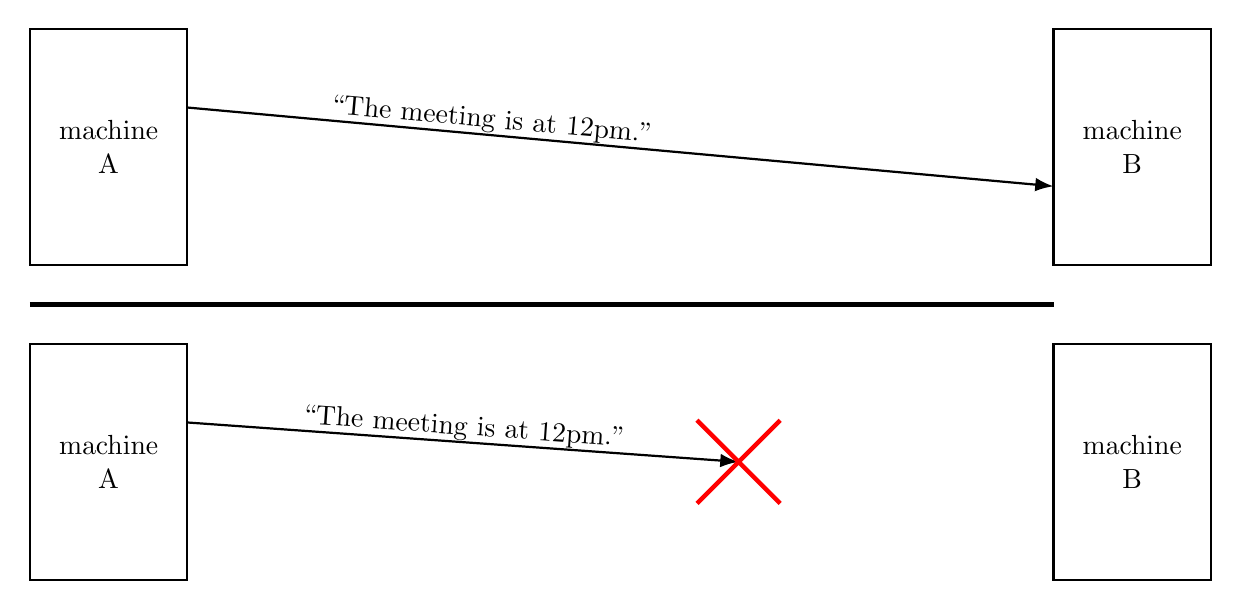
\begin{tikzpicture}
\tikzset{
    box/.style={draw,thick,minimum width=2cm},
    message/.style={draw,thick,-Latex},
    failure/.style={draw,ultra thick,red,cross out,minimum width=1cm,minimum height=1cm},
}
\begin{scope}
\draw[box] (0, 0) rectangle ++(2, -3) 
    node[midway,align=center] {machine\\ A};
\draw[box] (13, 0) rectangle ++(2, -3) 
    node[midway,align=center] {machine\\B};
\draw[message] (2, -1) -- (13, -2) node[pos=0.35, above, sloped] {``The meeting is at 12pm.''};
\end{scope}
\draw[ultra thick] (0, -3.5) -- ++ (13,0);
\begin{scope}[yshift=-4cm]
\draw[box] (0, 0) rectangle ++(2, -3) 
    node[midway,align=center] {machine\\A};
\draw[box] (13, 0) rectangle ++(2, -3) 
    node[midway,align=center] {machine\\B};
\draw[message] (2, -1) -- (9, -1.5) 
    node[pos=0.5,above,sloped] {``The meeting is at 12pm.''}
    node[failure] {};
\end{scope}
\end{tikzpicture}
\end{frame}

\begin{frame}{handling lost message: acknowledgements}
\begin{tikzpicture}
\tikzset{
    box/.style={thick},
    message/.style={draw,thick,-Latex},
    failure/.style={draw,ultra thick,red,cross out,minimum width=1cm,minimum height=1cm},
}
\begin{scope}
\draw[box] (0, 0) rectangle ++(2, -8) 
    node[midway,align=center] {machine\\A};
\draw[box] (13, 0) rectangle ++(2, -8) 
    node[midway,align=center] {machine\\B};
\draw[message] (2, -0.5) -- (13, -1) node[pos=0.35, above, sloped] {``The meeting is at 12pm.''};
\draw[message] (13, -1.5) -- (2, -2) node[pos=0.25, sloped,below] {Got it!};
\end{scope}
\end{tikzpicture}
\end{frame}

\begin{frame}{handling lost message}
\begin{tikzpicture}
\tikzset{
    box/.style={thick},
    message/.style={draw,thick,-Latex},
    failure/.style={draw,ultra thick,red,cross out,minimum width=1cm,minimum height=1cm},
}
\draw[box] (0, 0) rectangle ++(2, -8) 
    node[midway,align=center] {machine\\A};
\draw[box] (13, 0) rectangle ++(2, -8) 
    node[midway,align=center] {machine\\B};
%\draw[message] (2, -0.5) -- (13, -1) node[pos=0.35, above, sloped] {``The meeting is at 12pm.''};
\draw[message] (2, -0.5) -- (9, -1) 
    node[pos=0.5,above,sloped] {``The meeting is at 12pm.''}
    node[failure] {};
\begin{visibleenv}<2->
\draw[decorate,decoration={brace}] (2.1, -1) -- (2.1, -3) 
    node[midway,right,align=left] {
        ``timeout'' \\
        A doesn't get reply \\
        after waiting too long
    };
\end{visibleenv}
\begin{visibleenv}<3->
\draw[message] (2, -4) -- (13, -5) node[pos=0.35, above, sloped] {``The meeting is at 12pm.''};
\draw[message] (13, -5.5) -- (2, -6) node[pos=0.5, sloped,below] {Got it!};
\end{visibleenv}
\end{tikzpicture}
\end{frame}

\begin{frame}{protocol so far}
    \begin{itemize}
    \item on sender: until ACK received:
        \begin{itemize}
        \item (re)send frame of data
        \item wait fixed amount of time for ACK
        \end{itemize}
    \vspace{.5cm}
    \item on receiver: continuously:
        \begin{itemize}
        \item wait for frame of data
        \item send ACK back
        \end{itemize}
    \end{itemize}
\end{frame}


\subsection{sequence numbers}
\usetikzlibrary{arrows.meta,decorations.pathreplacing,shapes.misc}

\begin{frame}{problem}
    \begin{itemize}
    \item really want to send multiple frames
    \item example: data split in multiple pieces
    \end{itemize}
\end{frame}

\begin{frame}{splitting messages: try 1}
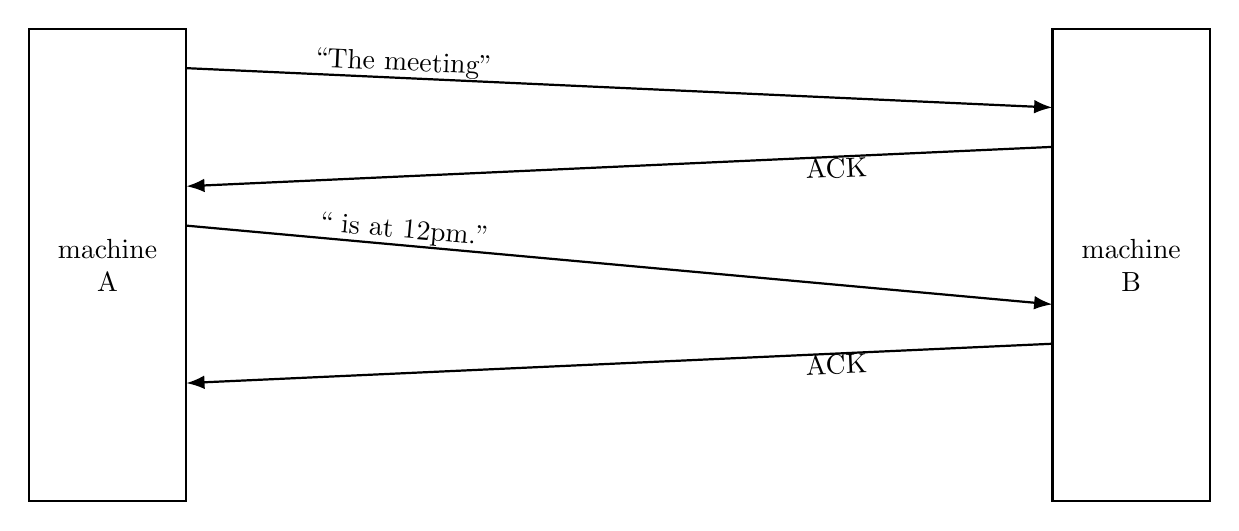
\begin{tikzpicture}
\tikzset{
    box/.style={thick},
    message/.style={draw,thick,-Latex},
    failure/.style={draw,ultra thick,red,cross out,minimum width=1cm,minimum height=1cm},
}
\begin{scope}
\draw[box] (0, 0) rectangle ++(2, -6) 
    node[midway,align=center] {machine\\A};
\draw[box] (13, 0) rectangle ++(2, -6) 
    node[midway,align=center] {machine\\B};
\draw[message] (2, -0.5) -- (13, -1) node[pos=0.25, above, sloped] {``The meeting''};
\draw[message] (13, -1.5) -- (2, -2) node[pos=0.25, sloped,below] {ACK};
\draw[message] (2, -2.5) -- (13, -3.5) node[pos=0.25, above, sloped] {`` is at 12pm.''};
\draw[message] (13, -4) -- (2, -4.5) node[pos=0.25, sloped,below] {ACK};
\end{scope}
\end{tikzpicture}
reconstructed message: \\
The meeting is at 12pm.
\end{frame}

\begin{frame}{splitting messages: try 1 --- problem 1}
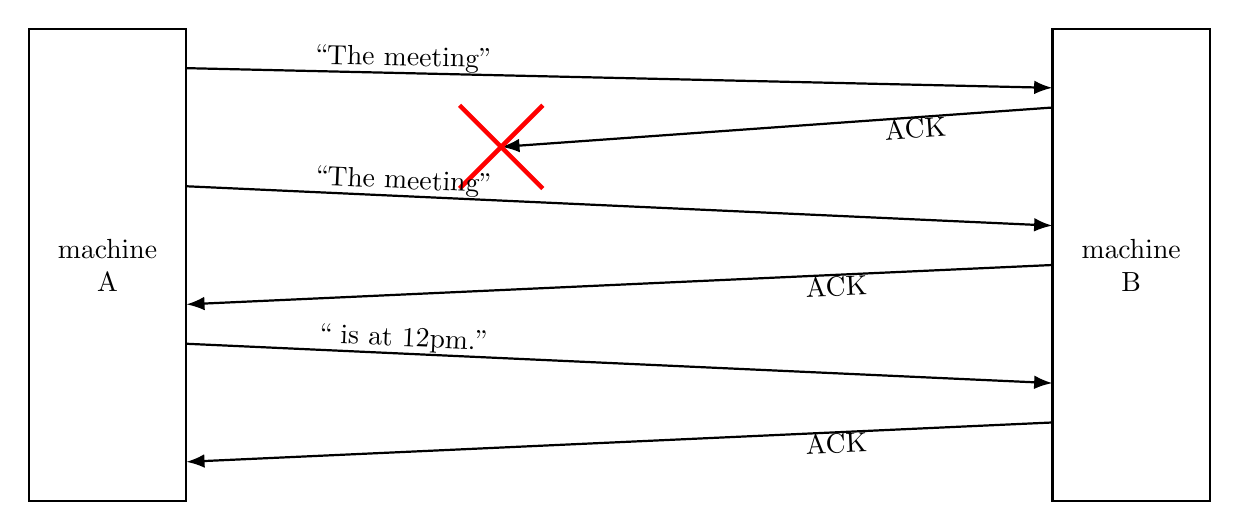
\begin{tikzpicture}
\tikzset{
    box/.style={thick},
    message/.style={draw,thick,-Latex},
    failure/.style={draw,ultra thick,red,cross out,minimum width=1cm,minimum height=1cm},
}
\begin{scope}
\draw[box] (0, 0) rectangle ++(2, -6) 
    node[midway,align=center] {machine\\A};
\draw[box] (13, 0) rectangle ++(2, -6) 
    node[midway,align=center] {machine\\B};
\draw[message] (2, -0.5) -- (13, -0.75) node[pos=0.25, above, sloped] {``The meeting''};
\draw[message] (13, -1) -- (6, -1.5) node[pos=0.25, sloped,below] {ACK} node[failure] {};
\draw[message] (2, -2) -- (13, -2.5) node[pos=0.25, above, sloped] {``The meeting''};
\draw[message] (13, -3) -- (2, -3.5) node[pos=0.25, sloped,below] {ACK};
\draw[message] (2, -4) -- (13, -4.5) node[pos=0.25, above, sloped] {`` is at 12pm.''};
\draw[message] (13, -5) -- (2, -5.5) node[pos=0.25, sloped,below] {ACK};
\end{scope}
\end{tikzpicture}
\begin{visibleenv}<2->
reconstructed message: \\
The meetingThe meeting is at 12pm.
\end{visibleenv}
\end{frame}

\begin{frame}{exercise: other problems?}
\begin{itemize}
\item sending `The meeting', `is at 12pm'
\item what would be received for each of these scenarios?
\end{itemize}
\begin{tabular}{ll}
1. & message (instead of acknowledgment) is lost \\
2. & first message from machine A is delayed a long time by network \\
3. & acknowledgment of second message lost instead of first \\
\end{tabular}
\end{frame}

\begin{frame}{aside: message delays}
    \begin{itemize}
    \item long message delays not possible with direct link
    \vspace{.5cm}
    \item but are possible with:
        \begin{itemize}
        \item multiple paths from A to B
        \item doing this kind of acknowledgment + resending hop-by-hop
        \end{itemize}
    \end{itemize}
\end{frame}

\begin{frame}{splitting messages: try 2}
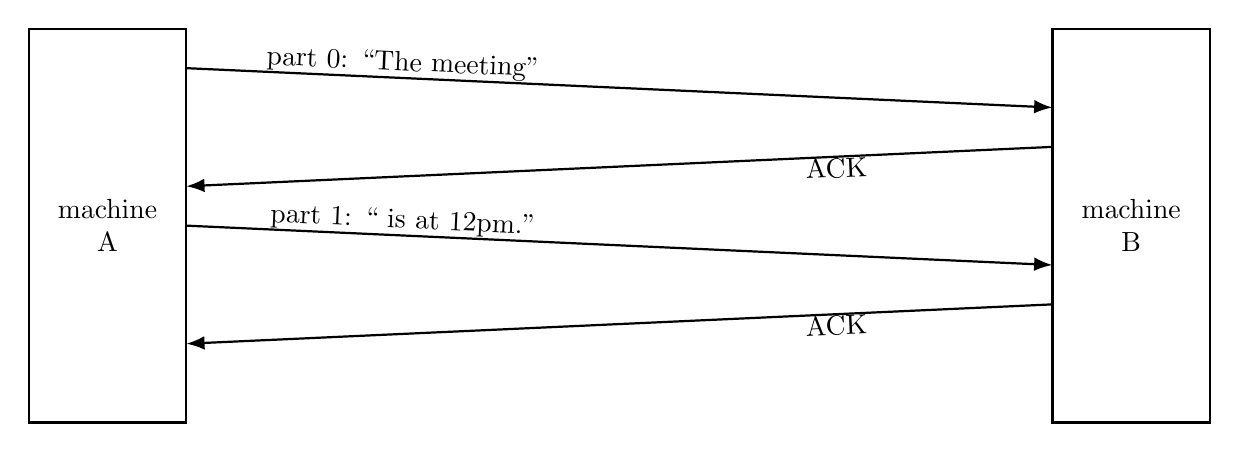
\begin{tikzpicture}
\tikzset{
    box/.style={thick},
    message/.style={draw,thick,-Latex},
    failure/.style={draw,ultra thick,red,cross out,minimum width=1cm,minimum height=1cm},
}
\begin{scope}
\draw[box] (0, 0) rectangle ++(2, -5) 
    node[midway,align=center] {machine\\A};
\draw[box] (13, 0) rectangle ++(2, -5) 
    node[midway,align=center] {machine\\B};
\draw[message] (2, -0.5) -- (13, -1) node[pos=0.25, above, sloped] {part 0: ``The meeting''};
\draw[message] (13, -1.5) -- (2, -2) node[pos=0.25, sloped,below] {ACK};
\draw[message] (2, -2.5) -- (13, -3) node[pos=0.25, above, sloped] {part 1: `` is at 12pm.''};
\draw[message] (13, -3.5) -- (2, -4) node[pos=0.25, sloped,below] {ACK};
\end{scope}
\end{tikzpicture}
reconstructed message: \\
The meeting is at 12pm.
\end{frame}

\begin{frame}{splitting messages: try 2 --- missed ack}
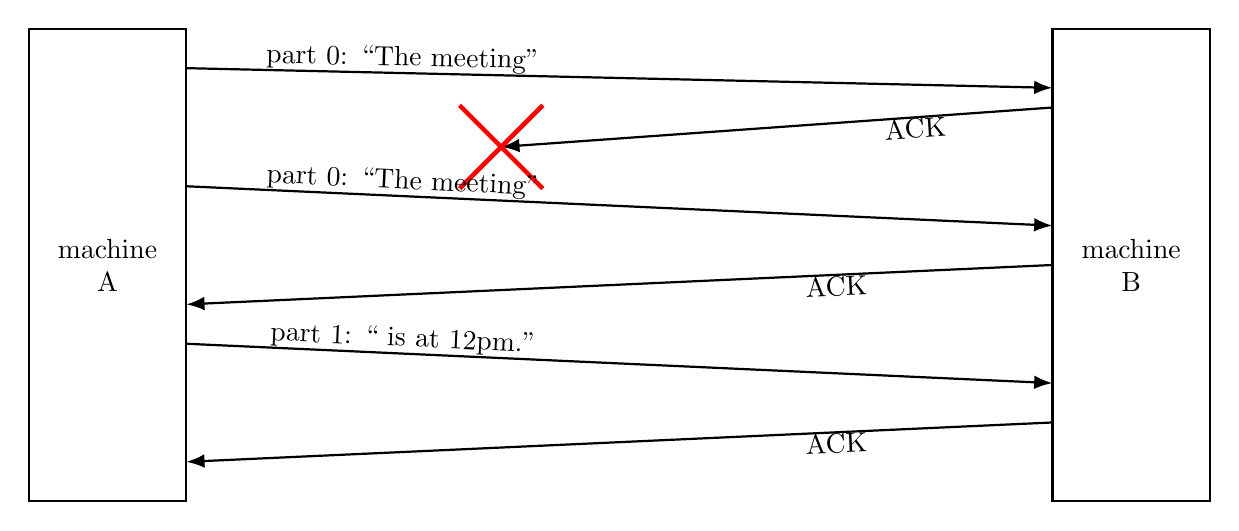
\begin{tikzpicture}
\tikzset{
    box/.style={thick},
    message/.style={draw,thick,-Latex},
    failure/.style={draw,ultra thick,red,cross out,minimum width=1cm,minimum height=1cm},
}
\begin{scope}
\draw[box] (0, 0) rectangle ++(2, -6) 
    node[midway,align=center] {machine\\A};
\draw[box] (13, 0) rectangle ++(2, -6) 
    node[midway,align=center] {machine\\B};
\draw[message] (2, -0.5) -- (13, -0.75) node[pos=0.25, above, sloped] {part 0: ``The meeting''};
\draw[message] (13, -1) -- (6, -1.5) node[pos=0.25, sloped,below] {ACK} node[failure] {};
\draw[message] (2, -2) -- (13, -2.5) node[pos=0.25, above, sloped] {part 0: ``The meeting''};
\draw[message] (13, -3) -- (2, -3.5) node[pos=0.25, sloped,below] {ACK};
\draw[message] (2, -4) -- (13, -4.5) node[pos=0.25, above, sloped] {part 1: `` is at 12pm.''};
\draw[message] (13, -5) -- (2, -5.5) node[pos=0.25, sloped,below] {ACK};
\end{scope}
\end{tikzpicture}
reconstructed message: \\
The meeting is at 12pm.
\end{frame}

\begin{frame}{splitting messages: try 2 --- problem}
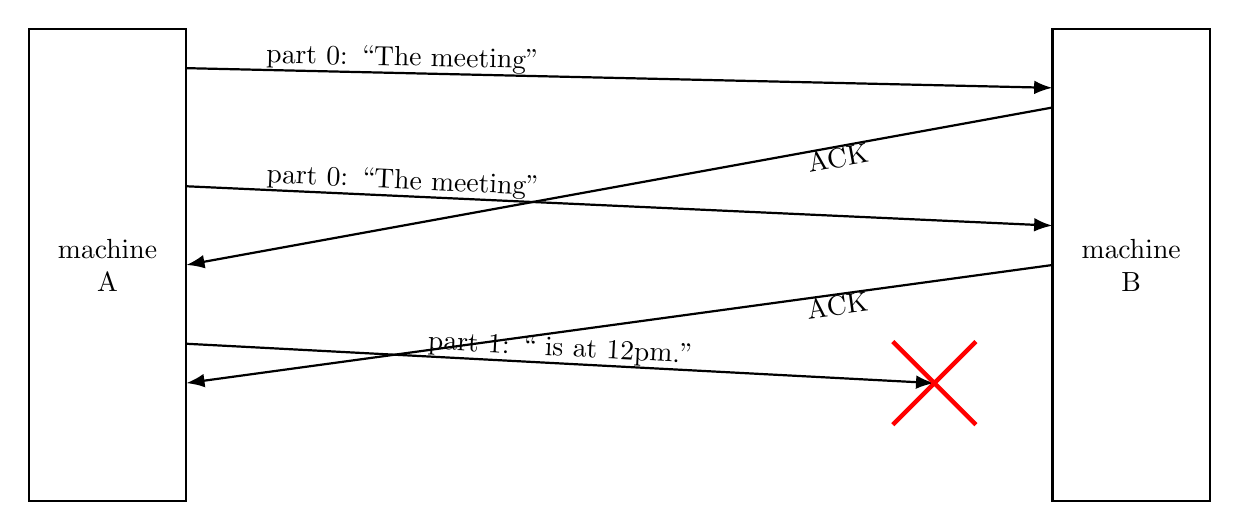
\begin{tikzpicture}
\tikzset{
    box/.style={thick},
    message/.style={draw,thick,-Latex},
    failure/.style={draw,ultra thick,red,cross out,minimum width=1cm,minimum height=1cm},
}
\begin{scope}
\draw[box] (0, 0) rectangle ++(2, -6) 
    node[midway,align=center] {machine\\A};
\draw[box] (13, 0) rectangle ++(2, -6) 
    node[midway,align=center] {machine\\B};
\draw[message] (2, -0.5) -- (13, -0.75) node[pos=0.25, above, sloped] {part 0: ``The meeting''};
\draw[message] (13, -1) -- (2, -3) node[pos=0.25, sloped,below] {ACK};
\draw[message] (2, -2) -- (13, -2.5) node[pos=0.25, above, sloped] {part 0: ``The meeting''};
\draw[message] (13, -3) -- (2, -4.5) node[pos=0.25, sloped,below] {ACK};
\draw[message] (2, -4) -- (11.5, -4.5) node[pos=0.5, above, sloped] {part 1: `` is at 12pm.''}
    node[failure] {};
\end{scope}
\end{tikzpicture}
A thinks: part 0 + part 1 acknowleged!
\end{frame}

\begin{frame}{splitting messages: version 3}
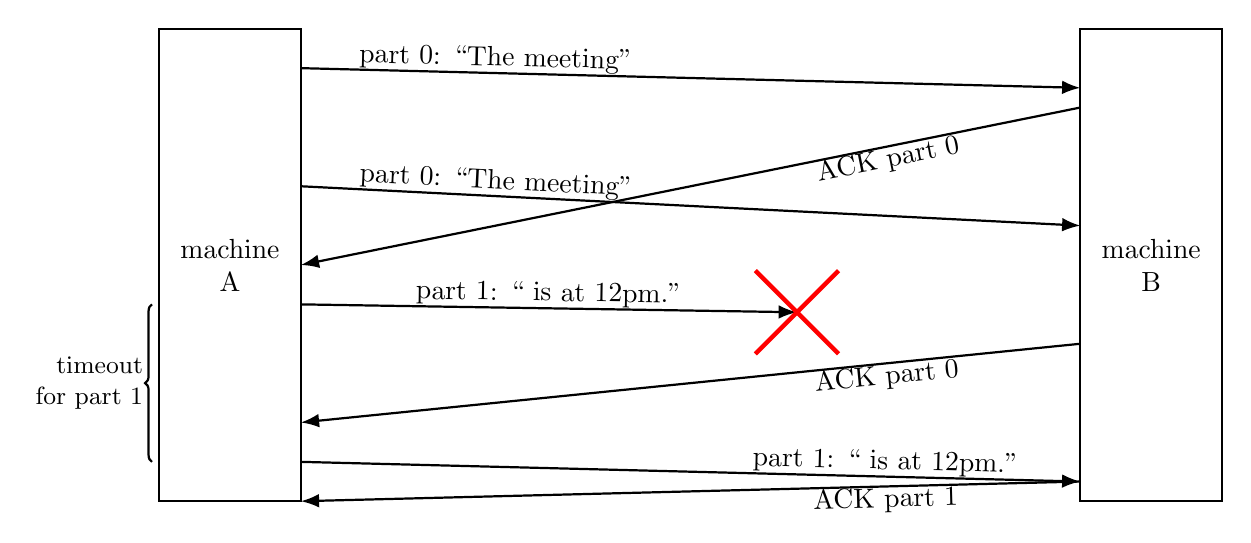
\begin{tikzpicture}
\tikzset{
    box/.style={thick},
    message/.style={draw,thick,-Latex},
    failure/.style={draw,ultra thick,red,cross out,minimum width=1cm,minimum height=1cm},
}
\begin{scope}[xshift=1cm,x=0.9cm]
\draw[box] (0, 0) rectangle ++(2, -6) 
    node[midway,align=center] {machine\\A};
\draw[box] (13, 0) rectangle ++(2, -6) 
    node[midway,align=center] {machine\\B};
\draw[message] (2, -0.5) -- (13, -0.75) node[pos=0.25, above, sloped] {part 0: ``The meeting''};
\draw[message] (13, -1) -- (2, -3) node[pos=0.25, sloped,below] {ACK \myemph{part 0}};
\draw[message] (2, -2) -- (13, -2.5) node[pos=0.25, above, sloped] {part 0: ``The meeting''};
\draw[message] (13, -4) -- (2, -5) node[pos=0.25, sloped,below] {ACK \myemph{part 0}};
\draw[message] (2, -3.5) -- (9, -3.6) node[pos=0.5, above, sloped] {part 1: `` is at 12pm.''}
    node[failure] {};
\draw[thick,decorate,decoration={brace,mirror}] (-0.1, -3.5) -- (-0.1, -5.5) node[inner sep=1mm,font=\small,align=right,midway,left] {timeout\\\myemph{for part 1}};
\draw[message] (2, -5.5) -- (13, -5.75) node[pos=0.75, above, sloped] {part 1: `` is at 12pm.''};
\draw[message] (13, -5.75) -- (2, -6) node[pos=0.25, below, sloped] {ACK \myemph{part 1}};
\end{scope}
\end{tikzpicture}
\end{frame}


\subsection{how many sequence numbers do we need?}
\providecommand\ttbox[1]{\fbox{\tt #1}}
\begin{frame}{sequence numbers}
    \begin{itemize}
    \item call the `part' label \textit{sequence number}
        \begin{itemize}
        \item for now: sequence number = message (or \textit{segment}) number
        \item in TCP: sequence number = byte number
        \end{itemize}
    \vspace{.5cm}
    \item important question: how large can they get?
    \item if we never reuse them --- infinite! 
    \item so \textit{really} want to reuse them
    \end{itemize}
\end{frame}

\begin{frame}{1-bit sequence number}
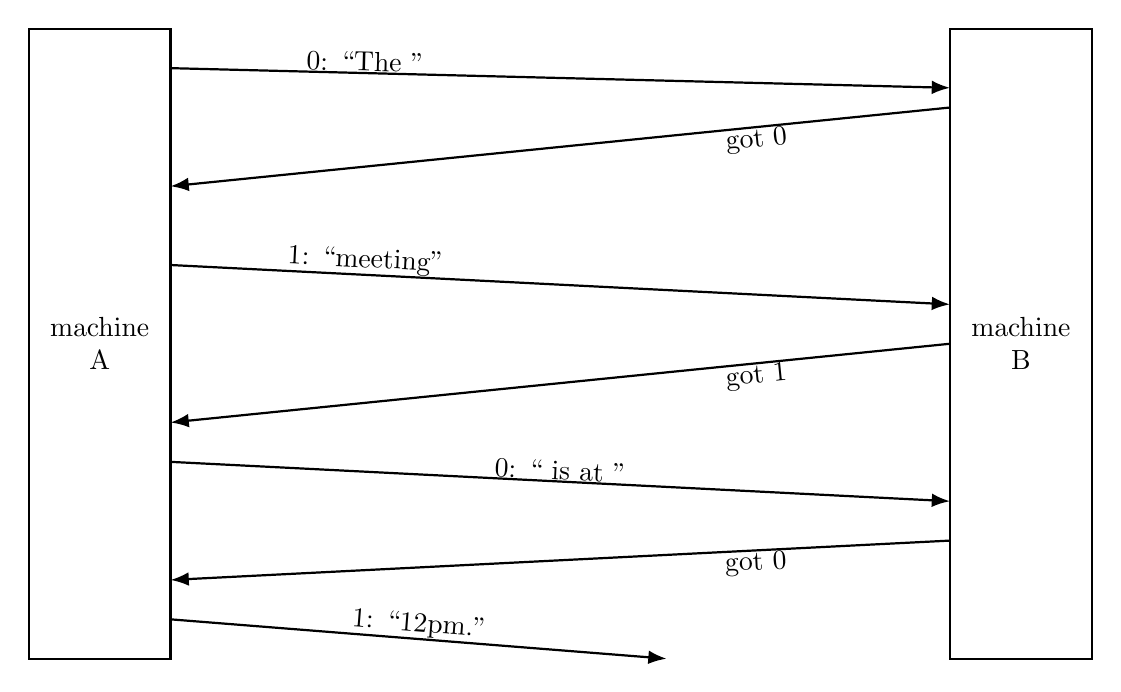
\begin{tikzpicture}
\tikzset{
    box/.style={thick},
    message/.style={draw,thick,-Latex},
    failure/.style={draw,ultra thick,red,cross out,minimum width=1cm,minimum height=1cm},
}
\begin{scope}[xshift=1cm,x=0.9cm]
\draw[box] (0, 0) rectangle ++(2, -8) 
    node[midway,align=center] {machine\\A};
\draw[box] (13, 0) rectangle ++(2, -8) 
    node[midway,align=center] {machine\\B};
\draw[message] (2, -0.5) -- (13, -0.75) node[pos=0.25, above, sloped] {\myemph{0}: ``The ''};
\draw[message] (13, -1) -- (2, -2) node[pos=0.25, sloped,below] {got \myemph{0}};
\draw[message] (2, -3) -- (13, -3.5) node[pos=0.25, above, sloped] {\myemph{1}: ``meeting''};
\draw[message] (13, -4) -- (2, -5) node[pos=0.25, sloped,below] {got \myemph{1}};
\draw[message] (2, -5.5) -- (13, -6) node[pos=0.5, above, sloped] {\myemph{0}: `` is at ''};
\draw[message] (13, -6.5) -- (2, -7) node[pos=0.25, sloped,below] {got \myemph{0}};
\draw[message] (2, -7.5) -- (9, -8) node[pos=0.5, above, sloped] {\myemph{1}: ``12pm.''};
\end{scope}
\end{tikzpicture}
\end{frame}

\begin{frame}{`stop and wait'}
    \begin{itemize}
    \item machine A is only sending \myemph{one thing at a time}
    \item never start sending next thing until after sending previous thing
    \end{itemize}
\end{frame}

\begin{frame}{stop-and-wait exercise (receive, 1)}
    \begin{itemize}
    \item machine B receives \ttbox{\myemph{0}: X}
    \item machine B sends \ttbox{got \myemph{0}}
    \item machine B receives \ttbox{\myemph{0}: X}
    \vspace{.5cm}
    \item what should machine B do now?
    \end{itemize}
\begin{tabular}{lll}
A. send \ttbox{got \myemph{0}} & B. send \ttbox{got \myemph{1}} & C. send nothing \\
\end{tabular}
\end{frame}

\begin{frame}{stop-and-wait exercise (receive, 2)}
    \begin{itemize}
    \item machine B receives \ttbox{\myemph{0}: X}
    \item machine B sends \ttbox{got \myemph{0}}
    \item machine B receives \ttbox{\myemph{1}: X}
    \vspace{.5cm}
    \item what should machine B do now?
    \end{itemize}
\begin{tabular}{lll}
A. send \ttbox{got \myemph{0}} & B. send \ttbox{got \myemph{1}} & C. send nothing \\
\end{tabular}
\end{frame}

\begin{frame}{stop-and-wait exercise (receive, 3)}
    \begin{itemize}
    \item machine B receives \ttbox{\myemph{0}: X}
    \item machine B sends \ttbox{got \myemph{0}}
    \item machine B receives \ttbox{\myemph{1}: Y}
    \item machine B sends \ttbox{got \myemph{1}}
    \item machine B receives \ttbox{\myemph{0}: X}
    \vspace{.5cm}
    \item what should machine B do now?
    \end{itemize}
\begin{tabular}{lll}
A. send \ttbox{got \myemph{0}} & B. send \ttbox{got \myemph{1}} & C. send nothing \\
\end{tabular}
\end{frame}


\begin{frame}{stop-and-wait exercise (send, 1)}
    \begin{itemize}
    \item A trying to send `X', then `Y', then `Z'
    \item machine A sends \ttbox{\myemph{0}: X}
    \item machine A sends \ttbox{\myemph{0}: X}
    \item machine A receives \ttbox{got \myemph{0}}
    \item machine A sends \ttbox{\myemph{1}: Y}
    \item machine A receives \ttbox{got \myemph{0}}
    \vspace{.5cm}
    \item what should machine A do now?
    \end{itemize}
\begin{tabular}{ll}
A. send \ttbox{0: X} again & B. send \ttbox{1: Y} again \\
C. send \ttbox{0: Z} & D. something else \\
\end{tabular}
\end{frame}

\begin{frame}{stop-and-wait exercise (send, 2)}
    \begin{itemize}
    \item A trying to send `X', then `Y', then `Z'
    \item machine A sends \ttbox{\myemph{0}: X}
    \item machine A sends \ttbox{\myemph{0}: X}
    \item machine A receives \ttbox{got \myemph{0}}
    \item machine A sends \ttbox{\myemph{1}: Y}
    \item machine A receives \ttbox{got \myemph{1}}
    \vspace{.5cm}
    \item what should machine A do now?
    \end{itemize}
\begin{tabular}{ll}
A. send \ttbox{\myemph{0}: X} again & B. send \ttbox{\myemph{1}: Y} again \\
C. send \ttbox{\myemph{0}: Z} & D. something else \\
\end{tabular}
\end{frame}


% FIXME: performance interlude

\section{interlude: metrics}
\begin{frame}{stop-and-wait issues}
    \begin{itemize}
    \item two issues with stop-and-wait:
    \vspace{.5cm}
    \item doesn't use close to full capacity of network
    \item not clear how to set timeouts
    \end{itemize}
\end{frame}

\begin{frame}{looking at metrics}
    \begin{itemize}
    \item several important metrics we'll care about
    \item (both for this and future topics)
    \vspace{.5cm}
    \item<2-> \textit{throughput} and \textit{bandwidth} ($\sim$ how much capacity used/available)
    \item<2-> \textit{latency} and \textit{round-trip time} (RTT) ($\sim$ what timeouts needed)
    \item<2-> \textit{jitter} ($\sim$ safety margin for timeouts)
    \end{itemize}
\end{frame}

\subsection{bandwidth / throughput}
\begin{frame}{bandwidth / throughput}
    \begin{itemize}
    \item bandwidth / data rate: maximum rate we can send per unit time
        \begin{itemize}
        \item most commonly measuring the speed of a link
        \end{itemize}
    \item 1 gigabit/second = transmit 1 bit / nanosecond
    \vspace{.5cm}
    \item throughput: acheived rate per unit time
        \begin{itemize}
        \item often lower than total bandwidth because of losses
        \item (we'll give several examples throughout the semester)
        \end{itemize}
    \end{itemize}
\end{frame}


\subsection{latency / round trip time}

\usetikzlibrary{arrows.meta,calc,shapes}
\providecommand{\computer}{%
    
\includegraphics[width=1cm]{../common/Noun_project_216.pdf}
}
\providecommand{\switch}{%
    
\includegraphics[width=0.9cm]{../common/fig-switch.pdf}
}
\providecommand{\router}{%
    
\includegraphics[width=0.9cm]{../common/fig-router.pdf}
}

\begin{frame}{latency (1)}
    \begin{itemize}
    \item latency: time for message: SOURCE $\rightarrow$ DEST
    \item example: \myemph<3>{1000} bit message from S to D:
    \end{itemize}
\begin{tikzpicture}
\tikzset{
    connect/.style={draw,very thick,Latex-Latex},
    computer/.style={inner sep=0mm,outer sep=0mm,execute at begin node={\computer}},
}
\node[computer,label={center:S}] (s) {};
\node[computer,label={center:D}] (d) at ([xshift=10cm]s.east) {};
\draw[connect] (s) -- (d) node[midway,above] {\myemph<2>{50 Mbit}, \myemph<3>{500 meters of copper}};
\end{tikzpicture}
\begin{itemize}
\item<2-> \myemph<2>{one} bit sent each \myemph<2>{1/50M second = 0.02 \mu s}
\item<2-> \myemph<3>{1000 bits take $0.02 \times 1000 = 20$ \mu s to sent}
    \begin{itemize}
    \item ``transmission delay''
    \end{itemize}
\item<3-> + $2.2$ microseconds for bit to go down cable ($2.3\times10^8$ m/s)
    \begin{itemize}
    \item ``propogation delay''
    \end{itemize}
\item<4-> total latency of about 22.2 \mu s
\end{itemize}
\end{frame}

\begin{frame}{latency (1, ex)}
\begin{tikzpicture}
\tikzset{
    connect/.style={draw,very thick,Latex-Latex},
    computer/.style={inner sep=0mm,outer sep=0mm,execute at begin node={\computer}},
    switch/.style={inner sep=0mm,outer sep=0mm,execute at begin node={\switch}},
}
\node[computer,label={center:S}] (s) {};
\node[computer,label={center:D}] (d) at ([xshift=10cm]s.east) {};
\draw[connect] (s) -- (d) node[midway,above] {\myemph{1 Gbit}, \myemph<3>{10 kilometers of fibre}};
\end{tikzpicture}
\begin{itemize}
\item exercise: latency for 20000 bit message from S to D
    \begin{itemize}
    \item assume speed of signal through fiber of $2.0\times10^8$ m/s
    \end{itemize}
\end{itemize}
\end{frame}

\begin{frame}{latency (2)}
    \begin{itemize}
    \item example: 1000 bit packet from S to D
    \item assume when message is received:
        \begin{itemize}
        \item 5 other 1000-bit packets in queue; no extra bits between packets
        \item no other switch processing time
        \end{itemize}
    \end{itemize}
\begin{tikzpicture}
\tikzset{
    connect/.style={draw,very thick,Latex-Latex},
    computer/.style={inner sep=0mm,outer sep=0mm,execute at begin node={\computer}},
    switch/.style={inner sep=0mm,outer sep=0mm,execute at begin node={\switch}},
}
\node[computer,label={center:S}] (s) {};
\node[switch] (m) at ([xshift=6.25cm]s.east) {};
\node[computer,label={center:D}] (d) at ([xshift=6.25cm]m.east) {};
\draw[connect] (s) -- (m) node[font=\small,midway,above] {50 Mbit, 500 meters of copper};
\draw[connect] (m) -- (d) node[font=\small,midway,above] {50 Mbit, 500 meters of copper};
\end{tikzpicture}
\vspace{-.5cm}
\begin{itemize}
\item S to switch, switch to D: 22.2 \mu s {\small (transmit+propogate delay)}
\item within switch: wait $20\times5=100$ \mu s for 5 other packets ($20\mu s$ = 1 packet transmit delay)
    \begin{itemize}
    \item ``queueing delay''
    \end{itemize}
\item total latency: $22.2 + 100 + 22.2 = 144.4$ microseconds
\end{itemize}
\end{frame}

\begin{frame}{round trip time}
    \begin{itemize}
    \item round-trip-time (RTT): time for message:  \\ SOURCE $\rightarrow$ DEST $\rightarrow$ SOURCE
    \vspace{.5cm}
    \item much easier to measure than one-way latency
    \item typically how we'll set latency
    \end{itemize}
\end{frame}


\subsection{jitter}
\begin{frame}{jitter}
\begin{itemize}
\item variation in latency
    \begin{itemize}
    \item most commonly from changing queuing delays
    \end{itemize}
\end{itemize}
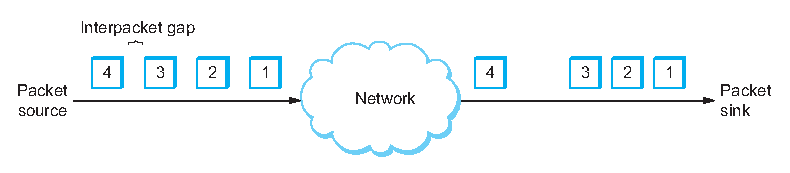
\includegraphics[width=0.9\textwidth]{../perf/SysApproach-1-Fig20}
\imagecredit{Figure 20 from Section 1.5 of \textit{Computer Networks: A Systems Approach} (6th ed) (Peterson and Davie)}
\end{frame}


\subsection{aside: measuring empirically}
\begin{frame}[fragile]{measuring round-trip time (1a)}
\begin{Verbatim}[fontsize=\fontsize{10}{11}]
charles@reisst14$ ping 1.1.1.1
PING 1.1.1.1 (1.1.1.1) 56(84) bytes of data.
64 bytes from 1.1.1.1: icmp_seq=1 ttl=52 time=13.8 ms
64 bytes from 1.1.1.1: icmp_seq=2 ttl=52 time=15.0 ms
64 bytes from 1.1.1.1: icmp_seq=3 ttl=52 time=12.5 ms
64 bytes from 1.1.1.1: icmp_seq=4 ttl=52 time=12.3 ms
64 bytes from 1.1.1.1: icmp_seq=5 ttl=52 time=13.5 ms
64 bytes from 1.1.1.1: icmp_seq=6 ttl=52 time=12.5 ms
64 bytes from 1.1.1.1: icmp_seq=7 ttl=52 time=13.3 ms
64 bytes from 1.1.1.1: icmp_seq=8 ttl=52 time=13.2 ms
64 bytes from 1.1.1.1: icmp_seq=9 ttl=52 time=13.3 ms
64 bytes from 1.1.1.1: icmp_seq=10 ttl=52 time=14.1 ms
^C
--- 1.1.1.1 ping statistics ---
10 packets transmitted, 10 received, 0% packet loss, time 9014ms
rtt min/avg/max/mdev = 12.273/13.343/15.024/0.786 ms
\end{Verbatim}
\end{frame}

\begin{frame}[fragile]{measuring round-trip-time (1b)}
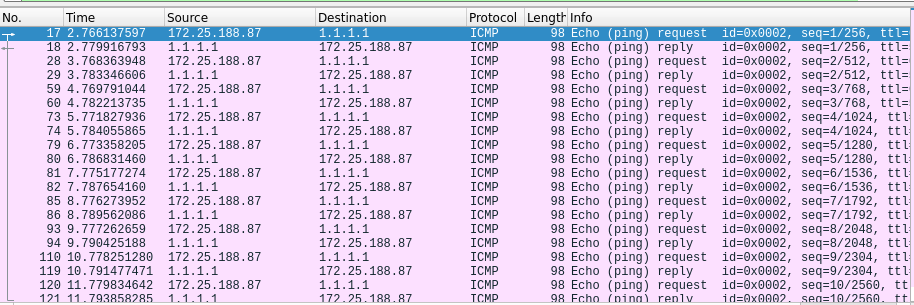
\includegraphics[width=\textwidth]{../perf/icmp-ping-pkts}
\end{frame}

\begin{frame}[fragile]{measuring round-trip-time (1c)}
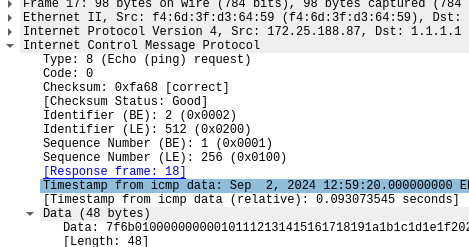
\includegraphics[width=\textwidth]{../perf/icmp-ping-pkt-example}
\end{frame}

\begin{frame}[fragile]{non-ICMP pings (1)}
\begin{Verbatim}[fontsize=\fontsize{10}{11}]
HPING www (enp0s31f6 128.143.67.8): NO FLAGS are set, 40 headers + 0 data bytes                          
len=46 ip=128.143.67.8 ttl=63 DF id=0 sport=0 flags=RA seq=0 win=0 rtt=3.5 ms                            
len=46 ip=128.143.67.8 ttl=63 DF id=0 sport=0 flags=RA seq=1 win=0 rtt=3.2 ms                            
len=46 ip=128.143.67.8 ttl=63 DF id=0 sport=0 flags=RA seq=2 win=0 rtt=7.1 ms                            
len=46 ip=128.143.67.8 ttl=63 DF id=0 sport=0 flags=RA seq=3 win=0 rtt=6.8 ms                            
len=46 ip=128.143.67.8 ttl=63 DF id=0 sport=0 flags=RA seq=4 win=0 rtt=6.5 ms                            
len=46 ip=128.143.67.8 ttl=63 DF id=0 sport=0 flags=RA seq=5 win=0 rtt=6.2 ms                            
len=46 ip=128.143.67.8 ttl=63 DF id=0 sport=0 flags=RA seq=6 win=0 rtt=5.8 ms                            
len=46 ip=128.143.67.8 ttl=63 DF id=0 sport=0 flags=RA seq=7 win=0 rtt=5.4 ms                            
len=46 ip=128.143.67.8 ttl=63 DF id=0 sport=0 flags=RA seq=8 win=0 rtt=5.0 ms                            
len=46 ip=128.143.67.8 ttl=63 DF id=0 sport=0 flags=RA seq=9 win=0 rtt=4.7 ms                            
^C                                                                                                       
--- www hping statistic ---                                                                              
10 packets transmitted, 10 packets received, 0% packet loss                                              
round-trip min/avg/max = 3.2/5.4/7.1 ms
\end{Verbatim}
\end{frame}

\begin{frame}[fragile]{non-ICMP pings (2)}
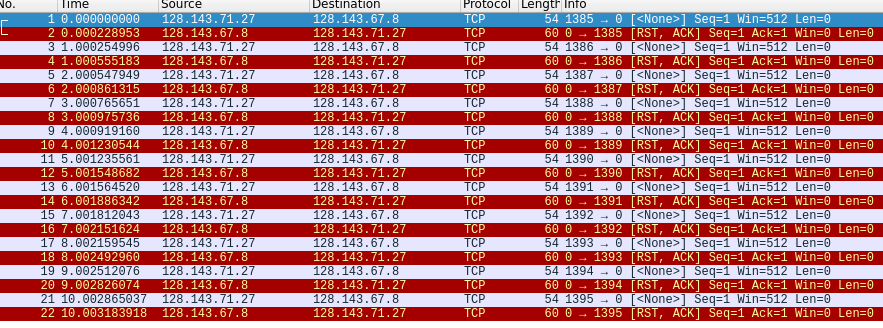
\includegraphics[width=\textwidth]{../perf/hping-wireshark}
\end{frame}

\begin{frame}[fragile]{measuring throughput?}
\begin{Verbatim}[fontsize=\fontsize{10}{11}]
$ scp test.dat portal.cs.virginia.edu:test.dat
test.dat                         100%   32MB  23.0MB/s   00:01    
$ scp portal.cs.virginia.edu:test.dat .
test.dat                         100%   32MB  28.2MB/s   00:01   
\end{Verbatim}
\begin{itemize}
\item (but might be measuring disk speed instead)
\vspace{.5cm}
\item also more specialized tools like \texttt{iperf}
    \begin{itemize}
    \item require program to run on both ends
    \end{itemize}
\end{itemize}
\end{frame}

\begin{frame}[fragile]{measuring transmission delay}
\begin{Verbatim}[fontsize=\fontsize{10}{11}]
$ ping -s 1400 www -i 0.05 -c 1000 -q
PING www.cs.virginia.edu (128.143.67.8) 1400(1428) bytes of data.
--- www.cs.virginia.edu ping statistics ---
1000 packets transmitted, 1000 received, 0% packet loss, time 50638ms
rtt min/avg/max/mdev = 0.319/0.461/1.222/0.039 ms
$ ping -s 16 www -i 0.05 -c 1000 -q
PING www.cs.virginia.edu (128.143.67.8) 16(44) bytes of data.
--- www.cs.virginia.edu ping statistics ---
1000 packets transmitted, 1000 received, 0% packet loss, time 50995ms
rtt min/avg/max/mdev = 0.156/0.345/1.539/0.068 ms
\end{Verbatim}
\begin{itemize}
\item approx. $0.416 - 0.345 = 0.071$ ms delay for $1400-16$ extra bytes
    \begin{itemize}
    \item with two links in each direction = approx $\frac{0.071}{4}=0.018$ ms/link
    \item $\frac{1400-16 \text{byte}}{0.018 \text{ms}} \approx 600$ Mbit/sec
    \item very noisy; true value probably 1 Gbit/sec
    \end{itemize}
\end{itemize}
\end{frame}


\section{stop-and-wait performance}
\begin{frame}{stop-and-wait performance}
    \begin{itemize}
    \item stop-and-wait protocol
    \item assuming no packets lost/corrupted
    \vspace{.5cm}
    \item about \myemph{one packet per round-trip time}
    \end{itemize}
\end{frame}

\begin{frame}{example: local ethernet}
    \begin{itemize}
    \item my home wired network: 0.6 ms round trip time
    \item typical packet has about 1400 bytes = 11200 bits of data
    \item throughput with stop-and-wait: $11200 \text{b} / 0.6 \text{ms} \approx 19000 \text{b/ms} = 19\;000\;000 \text{b/s} = \myemph<2>{19 \text{Mbit/s}}$
    \vspace{.5cm}
    \item available bandwidth is about \myemph<2>{$1$ Gbit/s}
    \end{itemize}
\end{frame}


\section{sliding windows}

\subsection{sending two at a time}

\usetikzlibrary{arrows.meta,shapes.misc}
\begin{frame}{sending two at a time}
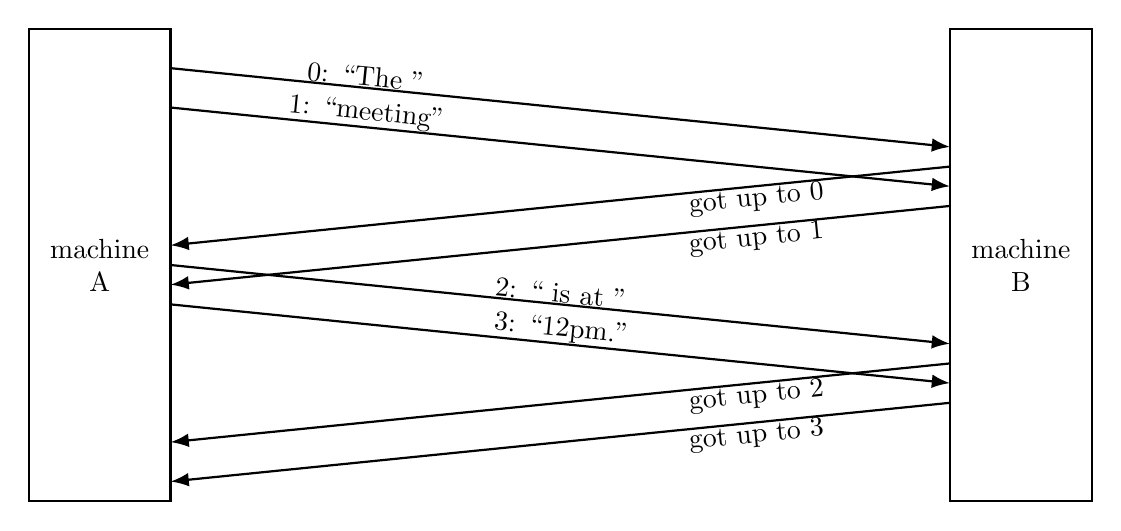
\begin{tikzpicture}
\tikzset{
    box/.style={thick},
    message/.style={draw,thick,-Latex},
    failure/.style={draw,ultra thick,red,cross out,minimum width=1cm,minimum height=1cm},
    every node/.style={inner sep=0.1mm},
}
\begin{scope}[xshift=1cm,x=0.9cm]
\draw[box] (0, 0) rectangle ++(2, -6) 
    node[midway,align=center] {machine\\A};
\draw[box] (13, 0) rectangle ++(2, -6) 
    node[midway,align=center] {machine\\B};
\draw[message] (2, -0.5) -- (13, -1.5) node[pos=0.25,above,sloped] {\myemph{0}: ``The ''};
\draw[message] (13, -1.75) -- (2, -2.75) node[pos=0.25,sloped,below] {got up to \myemph{0}};
\draw[message] (2, -1) -- (13, -2) node[pos=0.25, above, sloped] {\myemph{1}: ``meeting''};
\draw[message] (13, -2.25) -- (2, -3.25) node[pos=0.25, sloped,below] {got up to \myemph{1}};

% in response to got 0
\draw[message] (2, -3) -- (13, -4) node[pos=0.5, above, sloped] {\myemph{2}: `` is at ''};
\draw[message] (13, -4.25) -- (2, -5.25) node[pos=0.25, sloped,below] {got up to \myemph{2}};
% in response to got 1
\draw[message] (2, -3.5) -- (13, -4.5) node[pos=0.5, above, sloped] {\myemph{3}: ``12pm.''};
\draw[message] (13, -4.75) -- (2, -5.75) node[pos=0.25, sloped,below] {got up to \myemph{3}};
\end{scope}
\end{tikzpicture}
\begin{itemize}
\item key idea: always have two in flight
\item send next when previous ack'd
\end{itemize}
\end{frame}


\subsection{timeouts for EACH send}
\begin{frame}{timeouts per message} 
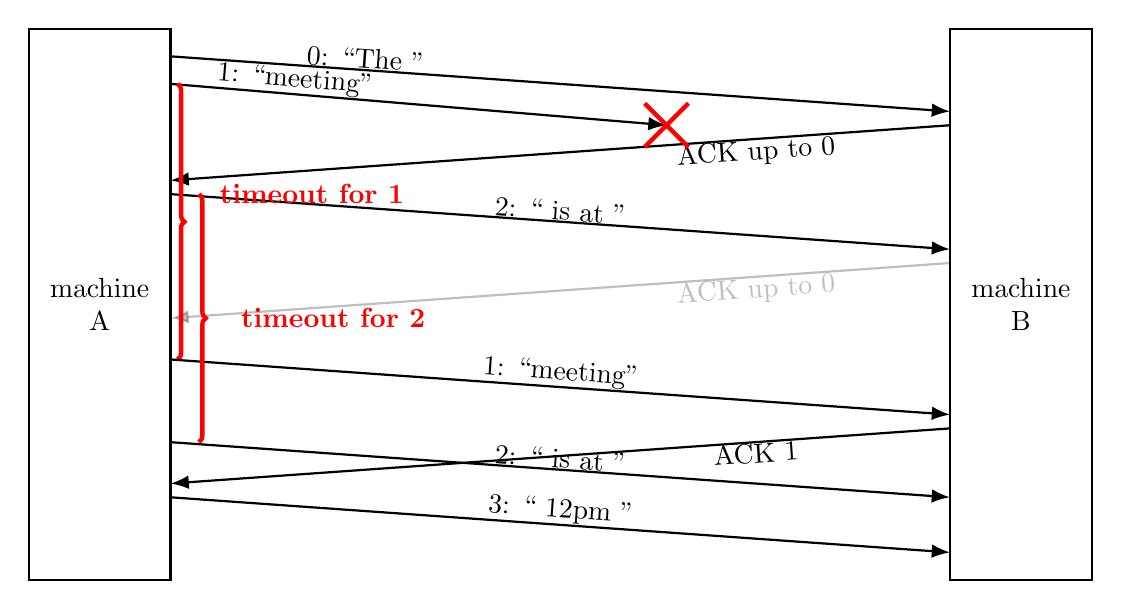
\begin{tikzpicture}
\tikzset{
    box/.style={thick},
    message/.style={draw,thick,-Latex},
    failure/.style={draw,ultra thick,red,cross out,minimum width=.5cm,minimum height=.5cm},
    every node/.style={inner sep=0.1mm},
}
\begin{scope}[xshift=1cm,x=0.9cm,y=0.7cm]
\draw[box] (0, 0) rectangle ++(2, -10) 
    node[midway,align=center] {machine\\A};
\draw[box] (13, 0) rectangle ++(2, -10) 
    node[midway,align=center] {machine\\B};
\draw[message] (2, -0.5) -- (13, -1.5) node[pos=0.25,above,sloped] {\myemph{0}: ``The ''};
\draw[message] (13, -1.75) -- (2, -2.75) node[pos=0.25,sloped,below] {ACK up to \myemph{0}};
\draw[message] (2, -1) -- (9, -1.75) node[pos=0.25, above, sloped] {\myemph{1}: ``meeting''}
    node[failure] {};
%\draw[message] (13, -2.25) -- (2, -3.25) node[pos=0.25, sloped,below] {got \myemph{1}};

% in response to got 0
\draw[message] (2, -3) -- (13, -4) node[pos=0.5, above, sloped] {\myemph{2}: `` is at ''};
%\draw[message] (13, -4.25) -- (2, -5.25) node[pos=0.25, sloped,below,alt=<2>{draw=red,ultra thick}] {ACK up to \myemph{0}};
\draw[message,opacity=0.25] (13, -4.25) -- (2, -5.25) node[pos=0.25, sloped,below] {ACK up to \myemph{0}};

\draw[ultra thick,red,decorate,decoration={brace}] (2.1, -1) -- (2.1, -6) node[pos=0.4,right=0.5cm] {\bfseries timeout for 1};
\draw[message] (2, -6) -- (13, -7) node[pos=0.5, above, sloped] {\myemph{1}: ``meeting''};
\draw[message] (13, -7.25) -- (2, -8.25) node[pos=0.25, sloped,below] {ACK \myemph{1}};
\draw[message] (2, -8.5) -- (13, -9.5) node[pos=0.5, above, sloped] {\myemph{3}: `` 12pm ''};

\draw[ultra thick,red,decorate,decoration={brace}] (2.4, -3) -- (2.4, -7.5) node[pos=0.5,right=0.5cm] {\bfseries timeout for 2};
\draw[message] (2, -7.5) -- (13, -8.5) node[pos=0.5, above, sloped] {\myemph{2}: `` is at ''};
\end{scope}
\end{tikzpicture}
\end{frame}


\subsection{more than two at a time}
\begin{frame}{sending three at a time}
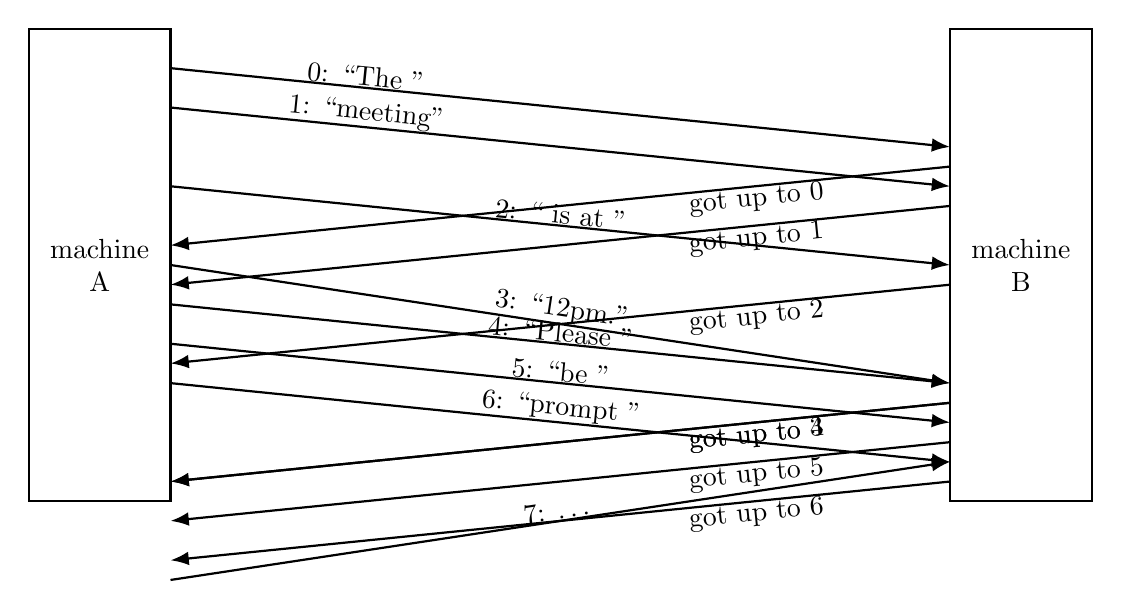
\begin{tikzpicture}
\tikzset{
    box/.style={thick},
    message/.style={draw,thick,-Latex},
    failure/.style={draw,ultra thick,red,cross out,minimum width=1cm,minimum height=1cm},
    every node/.style={inner sep=0.1mm},
}
\begin{scope}[xshift=1cm,x=0.9cm]
\draw[box] (0, 0) rectangle ++(2, -6) 
    node[midway,align=center] {machine\\A};
\draw[box] (13, 0) rectangle ++(2, -6) 
    node[midway,align=center] {machine\\B};
\draw[message] (2, -0.5) -- (13, -1.5) node[pos=0.25,above,sloped] {\myemph{0}: ``The ''};
\draw[message] (13, -1.75) -- (2, -2.75) node[pos=0.25,sloped,below] {got up to \myemph{0}};
\draw[message] (2, -1) -- (13, -2) node[pos=0.25, above, sloped] {\myemph{1}: ``meeting''};
\draw[message] (13, -2.25) -- (2, -3.25) node[pos=0.25, sloped,below] {got up to \myemph{1}};
\draw[message] (2, -2) -- (13, -3) node[pos=0.5, above, sloped] {\myemph{2}: `` is at ''};
\draw[message] (13, -3.25) -- (2, -4.25) node[pos=0.25, sloped,below] {got up to \myemph{2}};
% in response to got 0
\draw[message] (2, -3) -- (13, -4.5) node[pos=0.5, above, sloped] {\myemph{3}: ``12pm.''};
\draw[message] (13, -4.75) -- (2, -5.75) node[pos=0.25, sloped,below] {got up to \myemph{3}};
% in response to got 1 
\draw[message] (2, -3.5) -- (13, -4.5) node[pos=0.5, above, sloped] {\myemph{4}: ``Please ''};
\draw[message] (13, -4.75) -- (2, -5.75) node[pos=0.25, sloped,below] {got up to \myemph{4}};
\draw[message] (2, -4) -- (13, -5) node[pos=0.5, above, sloped] {\myemph{5}: ``be ''};
\draw[message] (13, -5.25) -- (2, -6.25) node[pos=0.25, sloped,below] {got up to \myemph{5}};
\draw[message] (2, -4.5) -- (13, -5.5) node[pos=0.5, above, sloped] {\myemph{6}: ``prompt ''};
\draw[message] (13, -5.75) -- (2, -6.75) node[pos=0.25, sloped,below] {got up to \myemph{6}};
\draw[message] (2, -7) -- (13, -5.5) node[pos=0.5, above, sloped] {\myemph{7}: \ldots};
\end{scope}
\end{tikzpicture}
\begin{itemize}
\item choose ``window size'' to have in flight
\item send when previous acknowledged
\end{itemize}
\end{frame}


\subsection{lost ACKs}
\begin{frame}{lost ACKs?}
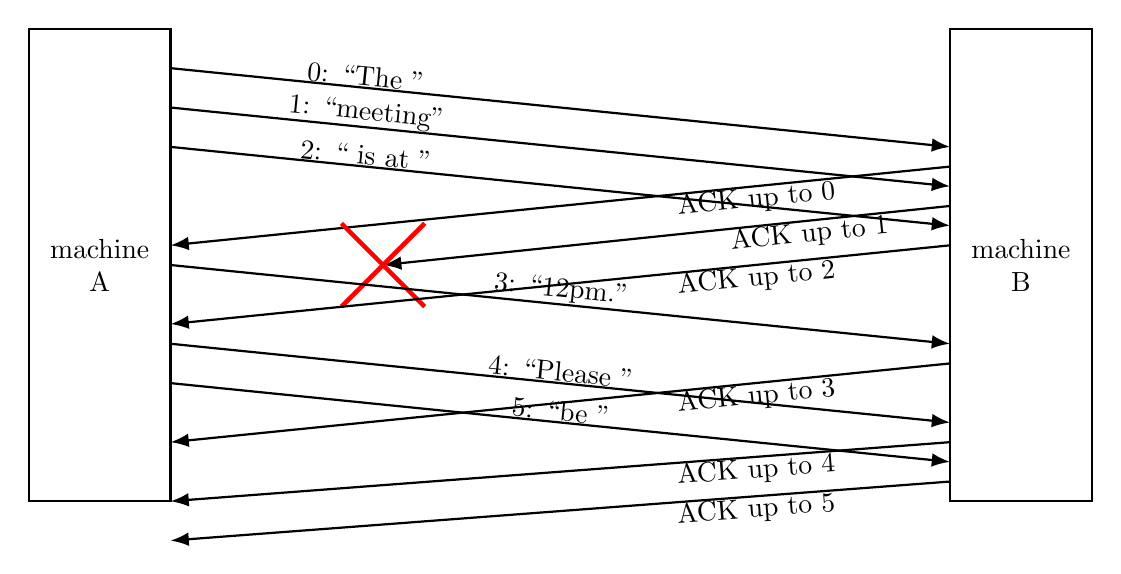
\begin{tikzpicture}
\tikzset{
    box/.style={thick},
    message/.style={draw,thick,-Latex},
    failure/.style={draw,ultra thick,red,cross out,minimum width=1cm,minimum height=1cm},
    every node/.style={inner sep=0.1mm},
}
\begin{scope}[xshift=1cm,x=0.9cm]
\draw[box] (0, 0) rectangle ++(2, -6) 
    node[midway,align=center] {machine\\A};
\draw[box] (13, 0) rectangle ++(2, -6) 
    node[midway,align=center] {machine\\B};
\draw[message] (2, -0.5) -- (13, -1.5) node[pos=0.25,above,sloped] {\myemph{0}: ``The ''};
\draw[message] (13, -1.75) -- (2, -2.75) node[pos=0.25,sloped,below] {ACK up to \myemph{0}};
\draw[message] (2, -1) -- (13, -2) node[pos=0.25, above, sloped] {\myemph{1}: ``meeting''};
\draw[message] (13, -2.25) -- (5, -3) node[pos=0.25, sloped,below] {ACK up to \myemph{1}} node[failure] {};
\draw[message] (2, -1.5) -- (13, -2.5) node[pos=0.25, above, sloped] {\myemph{2}: `` is at ''};
\draw[message] (13, -2.75) -- (2, -3.75) node[pos=0.25, sloped,below] {ACK up to \myemph{2}};
\draw[message] (2, -3) -- (13, -4) node[pos=0.5, above, sloped] {\myemph{3}: ``12pm.''};
\draw[message] (13, -4.25) -- (2, -5.25) node[pos=0.25, sloped,below] {ACK up to \myemph{3}};
\draw[message] (2, -4) -- (13, -5) node[pos=0.5, above, sloped] {\myemph{4}: ``Please ''};
\draw[message] (13, -5.25) -- (2, -6) node[pos=0.25, sloped,below] {ACK up to \myemph{4}};
\draw[message] (2, -4.5) -- (13, -5.5) node[pos=0.5, above, sloped] {\myemph{5}: ``be ''};
\draw[message] (13, -5.75) -- (2, -6.5) node[pos=0.25, sloped,below] {ACK up to \myemph{5}};
%\draw[message] (2, -4.5) -- (13, -5.5) node[pos=0.5, above, sloped] {\myemph{6}: ``prompt ''};
%\draw[message] (13, -5.75) -- (2, -6.75) node[pos=0.25, sloped,below] {ACK up to \myemph{6}};
%\draw[message] (2, -7) -- (13, -5.5) node[pos=0.5, above, sloped] {\myemph{7}: \ldots};
\end{scope}
\end{tikzpicture}
\end{frame}


\subsection{duplicate ACKs happen}
    % FIXME: this would make more sense with more than two things
\usetikzlibrary{decorations.pathreplacing}
\begin{frame}<1-2>[label=twoAndTimeouts]{missing messages?}
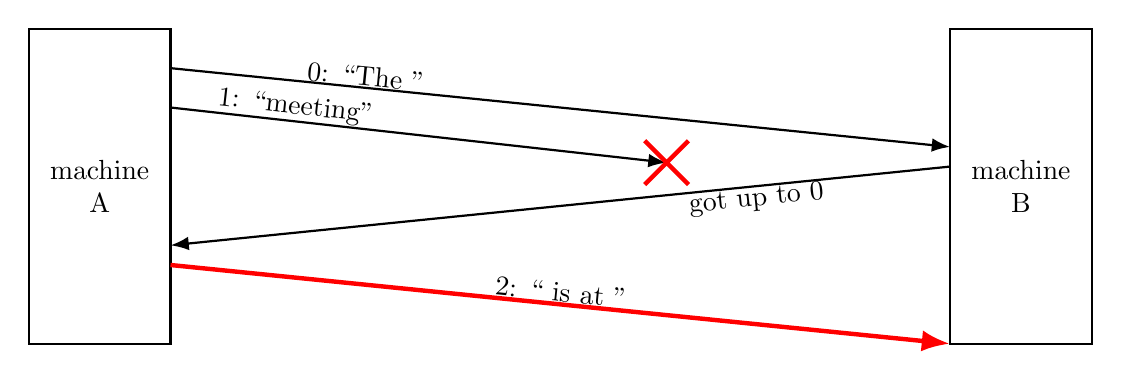
\begin{tikzpicture}
\tikzset{
    box/.style={thick},
    message/.style={draw,thick,-Latex},
    failure/.style={draw,ultra thick,red,cross out,minimum width=.5cm,minimum height=.5cm},
    every node/.style={inner sep=0.1mm},
}
\begin{scope}[xshift=1cm,x=0.9cm]
\draw[box] (0, 0) rectangle ++(2, -4) 
    node[midway,align=center] {machine\\A};
\draw[box] (13, 0) rectangle ++(2, -4) 
    node[midway,align=center] {machine\\B};
\draw[message] (2, -0.5) -- (13, -1.5) node[pos=0.25,above,sloped] {\myemph{0}: ``The ''};
\draw[message] (13, -1.75) -- (2, -2.75) node[pos=0.25,sloped,below] {got up to \myemph{0}};
\draw[message] (2, -1) -- (9, -1.7) node[pos=0.25, above, sloped] {\myemph{1}: ``meeting''}
    node[failure] {};
%\draw[message] (13, -2.25) -- (2, -3.25) node[pos=0.25, sloped,below] {got \myemph{1}};

% in response to got 0
\draw[message,draw=red,ultra thick] (2, -3) -- (13, -4) node[pos=0.5, above, sloped] {\myemph{2}: `` is at ''};
%\draw[message] (13, -4.25) -- (2, -5.25) node[pos=0.25, sloped,below,alt=<2>{draw=red,ultra thick}] {got up to \myemph{0}};
%\draw[message] (2, -3.5) -- (13, -4.5) node[pos=0.5, above, sloped] {\myemph{3}: ``12pm.''};
%\draw[message] (13, -4.75) -- (2, -5.75) node[pos=0.25, sloped,below] {got \myemph{3}};
\end{scope}
\end{tikzpicture}
\begin{itemize}
\item question: what should receiver do with sequence number 2?
\item<2-> \myemph<2>{one idea: ignore it?}
\item<3-> \myemph<3>{better idea: send something back to sender}
\end{itemize}
\end{frame}

\begin{frame}<0>{not great: ignore it (1)} 
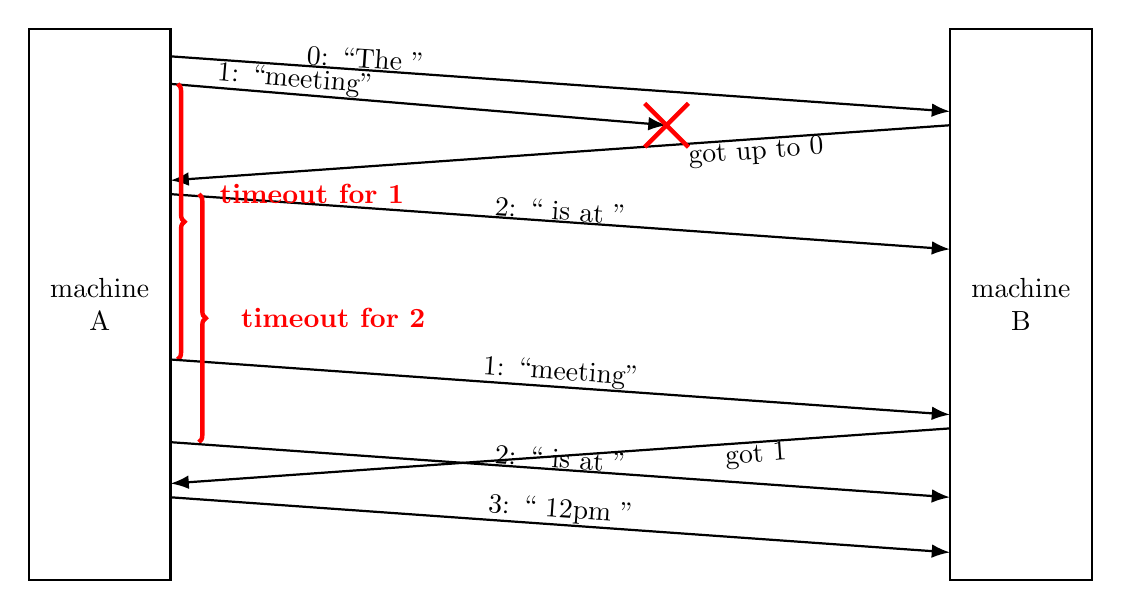
\begin{tikzpicture}
\tikzset{
    box/.style={thick},
    message/.style={draw,thick,-Latex},
    failure/.style={draw,ultra thick,red,cross out,minimum width=.5cm,minimum height=.5cm},
    every node/.style={inner sep=0.1mm},
}
\begin{scope}[xshift=1cm,x=0.9cm,y=0.7cm]
\draw[box] (0, 0) rectangle ++(2, -10) 
    node[midway,align=center] {machine\\A};
\draw[box] (13, 0) rectangle ++(2, -10) 
    node[midway,align=center] {machine\\B};
\draw[message] (2, -0.5) -- (13, -1.5) node[pos=0.25,above,sloped] {\myemph{0}: ``The ''};
\draw[message] (13, -1.75) -- (2, -2.75) node[pos=0.25,sloped,below] {got up to \myemph{0}};
\draw[message] (2, -1) -- (9, -1.75) node[pos=0.25, above, sloped] {\myemph{1}: ``meeting''}
    node[failure] {};
%\draw[message] (13, -2.25) -- (2, -3.25) node[pos=0.25, sloped,below] {got \myemph{1}};

% in response to got 0
\draw[message] (2, -3) -- (13, -4) node[pos=0.5, above, sloped] {\myemph{2}: `` is at ''};
%\draw[message] (13, -4.25) -- (2, -5.25) node[pos=0.25, sloped,below,alt=<2>{draw=red,ultra thick}] {got up to \myemph{0}};
\draw[ultra thick,red,decorate,decoration={brace}] (2.1, -1) -- (2.1, -6) node[pos=0.4,right=0.5cm] {\bfseries timeout for 1};
\draw[message] (2, -6) -- (13, -7) node[pos=0.5, above, sloped] {\myemph{1}: ``meeting''};
\draw[message] (13, -7.25) -- (2, -8.25) node[pos=0.25, sloped,below] {got \myemph{1}};
\draw[message] (2, -8.5) -- (13, -9.5) node[pos=0.5, above, sloped] {\myemph{3}: `` 12pm ''};

\draw[ultra thick,red,decorate,decoration={brace}] (2.4, -3) -- (2.4, -7.5) node[pos=0.5,right=0.5cm] {\bfseries timeout for 2};
\draw[message] (2, -7.5) -- (13, -8.5) node[pos=0.5, above, sloped] {\myemph{2}: `` is at ''};
\end{scope}
\end{tikzpicture}
\end{frame}

\begin{frame}<0>{not great: only ACK if next (2)}
    \begin{itemize}
    \item \textit{works} because we still have timeouts
    \vspace{.5cm}
    \item but we'd like to give more feedback to receiver
    \end{itemize}
\end{frame}

\againframe<3>{twoAndTimeouts}

\begin{frame}{better idea: always ACK}
\begin{tikzpicture}
\tikzset{
    box/.style={thick},
    message/.style={draw,thick,-Latex},
    failure/.style={draw,ultra thick,red,cross out,minimum width=1cm,minimum height=1cm},
    every node/.style={inner sep=0.1mm},
}
\begin{scope}[xshift=1cm,x=0.9cm]
\draw[box] (0, 0) rectangle ++(2, -5.5) 
    node[midway,align=center] {machine\\A};
\draw[box] (13, 0) rectangle ++(2, -5.5) 
    node[midway,align=center] {machine\\B};
\draw[message] (2, -0.5) -- (13, -1.5) node[pos=0.25,above,sloped] {\myemph{0}: ``The ''};
\draw[message] (13, -1.75) -- (2, -2.75) node[pos=0.25,sloped,below] {got up to \myemph{0}};
\draw[message] (2, -1) -- (9, -1.7) node[pos=0.25, above, sloped] {\myemph{1}: ``meeting''}
    node[failure] {};
%\draw[message] (13, -2.25) -- (2, -3.25) node[pos=0.25, sloped,below] {got \myemph{1}};

% in response to got 0
\draw[message] (2, -3) -- (13, -4) node[pos=0.5, above, sloped] {\myemph{2}: `` is at ''};
\draw[message] (13, -4.25) -- (2, -5.25) node[pos=0.25, sloped,below,alt=<2>{draw=red,ultra thick}] {got up to \myemph{0}};
%\draw[message] (2, -3.5) -- (13, -4.5) node[pos=0.5, above, sloped] {\myemph{3}: ``12pm.''};
%\draw[message] (13, -4.75) -- (2, -5.75) node[pos=0.25, sloped,below] {got \myemph{3}};
\end{scope}
\end{tikzpicture}
\begin{itemize}
\item<2-> only ACK $x$ if \myemph{everything up to and including $x$} received
\item<2-> intuition: ACK tells sender \myemph{where to start sending more}
\end{itemize}
\end{frame}


\subsection{duplicate ACK optimization}
\begin{frame}{fast retransmit}
    \begin{itemize}
    \item if large window + data packet 2 is lost, then sender will see
    \item ACK 0, \myemph{ACK 1, ACK 1, ACK 1, ACK 1, ACK 1}
    \item duplicate ACKs indicate missing packet 2
    \item \myemph{shouldn't wait for timeout}
    \vspace{.5cm}
    \item<2-> $\rightarrow$ TCP heuristic: retransmit immediately after $\sim$3 duplicate ACKs
        \begin{itemize}
        \item not 1 duplicate ACK to tolerate some reordering
        \item also some other details (we'll talk later)
        \end{itemize}
    \end{itemize}
\end{frame}



\subsection{optimization: selective ACKs}
\begin{frame}{multiple missing}
\begin{tikzpicture}
\tikzset{
    box/.style={thick},
    message/.style={draw,thick,-Latex},
    failure/.style={draw,ultra thick,red,cross out,minimum width=1cm,minimum height=1cm},
    every node/.style={inner sep=0.1mm},
}
\begin{scope}[xshift=1cm,x=0.9cm]
\draw[box] (0, 0) rectangle ++(2, -5.5) 
    node[midway,align=center] {machine\\A};
\draw[box] (13, 0) rectangle ++(2, -5.5) 
    node[midway,align=center] {machine\\B};
\draw[message] (2, -0.5) -- (13, -1.5) node[pos=0.25,above,sloped] {\myemph{0}: ``The ''};
\draw[message] (13, -1.75) -- (2, -2.75) node[pos=0.25,sloped,below] {got up to \myemph{0}};
\draw[message] (2, -1) -- (9, -1.7) node[pos=0.25, above, sloped] {\myemph{1}: ``meeting''}
    node[failure] {};
\draw[message] (2, -1.5) -- (13, -2) node[pos=0.5, above, sloped] {\myemph{2}: ``is''};
\draw[message] (2, -2) -- (13, -3) node[pos=0.5, above, sloped] {\myemph{3}: ``at''}
    node[failure] {};
\draw[message] (2, -3) -- (13, -4) node[pos=0.5, above, sloped] {\myemph{4}: ``12pm''};

\draw[message] (13, -2.25) -- (2, -3.25) node[pos=0.25, sloped,below,alt=<2>{draw=red,ultra thick}] {got up to \myemph{0}};
\draw[message] (13, -3.25) -- (2, -4.25) node[pos=0.25, sloped,below,alt=<2>{draw=red,ultra thick}] {got up to \myemph{0}};
\end{scope}
\end{tikzpicture}
\begin{itemize}
\item duplicate ACK heuristic will quickly resend 1, but not 3
\item would like to supply better information
\end{itemize}
\end{frame}

\begin{frame}{selective acknowledgments}
\begin{tikzpicture}
\tikzset{
    box/.style={thick},
    message/.style={draw,thick,-Latex},
    failure/.style={draw,ultra thick,red,cross out,minimum width=1cm,minimum height=1cm},
    every node/.style={inner sep=0.1mm},
}
\begin{scope}[xshift=1cm,x=0.9cm]
\draw[box] (0, 0) rectangle ++(2, -5.5) 
    node[midway,align=center] {machine\\A};
\draw[box] (13, 0) rectangle ++(2, -5.5) 
    node[midway,align=center] {machine\\B};
\draw[message] (2, -0.5) -- (13, -1.5) node[pos=0.25,above,sloped] {\myemph{0}: ``The ''};
\draw[message] (13, -1.75) -- (2, -2.75) node[pos=0.25,sloped,below] {got up to \myemph{0}};
\draw[message] (2, -1) -- (9, -1.7) node[pos=0.25, above, sloped] {\myemph{1}: ``meeting''}
    node[failure] {};
\draw[message] (2, -1.5) -- (13, -2) node[pos=0.5, above, sloped] {\myemph{2}: ``is''};
\draw[message] (2, -2) -- (13, -3) node[pos=0.5, above, sloped] {\myemph{3}: ``at''}
    node[failure] {};
\draw[message] (2, -3) -- (13, -4) node[pos=0.5, above, sloped] {\myemph{4}: ``12pm''};

\draw[message] (13, -2.25) -- (2, -3.25) node[pos=0.25, sloped,below,alt=<2>{draw=red,ultra thick}] {got up to \myemph{0} plus 2};
\draw[message] (13, -3.25) -- (2, -4.25) node[pos=0.25, sloped,below,alt=<2>{draw=red,ultra thick}] {got up to \myemph{0} plus 2 and 4};
\end{scope}
\end{tikzpicture}
\end{frame}

\begin{frame}{selective acknowledgments in TCP}
    \begin{itemize}
    \item optional feature (``extension'') described in RFC 2018
    \item send list of ranges received
    \item typically room for 3 ranges
    \item if more than 3 ranges to report, then:
        \begin{itemize}
        \item include range with most recently received frame
        \item include other ranges until sent three times
        \end{itemize}
    \end{itemize}
\end{frame}


\subsection{window tracking -- sender}
% FIXME: diagram of receiver, sender window
    % actions for each case
\usetikzlibrary{arrows.meta,decorations.pathreplacing,matrix,patterns}
\begin{frame}{sender window tracking}
\begin{tikzpicture}
\tikzset{
    seqlist/.style={tight matrix,nodes={text width=1cm,minimum height=1cm},column sep=.8mm},
    dots/.style={draw=none,execute at begin node=\ldots,anchor=center,font=\huge,text width=1cm,align=center},
    region mark/.style={very thick,decorate,decoration={brace,mirror}},
    region mark label/.style={midway,below,align=center},
    verified/.style={alt=<2->{pattern color=black!30,pattern=checkerboard}},
    in flight/.style={alt=<3->{fill=yellow}},
    unsent/.style={alt=<4->{pattern=crosshatch dots,pattern color=violet!70}}
}
\matrix[seqlist] (swindow) {
    |[dots,alias=swindow-start]| ~ \& |[alias=after-swindow-start,verified]| ~ \& |[verified]|  ~\&
   |[verified]| ~ \& |[alias=LFA,verified]| ~ \&
    |[in flight,alias=after LFA]| ~ \& |[in flight]| ~ \& |[in flight]| ~ \& |[in flight,alias=LFS]| ~ \& 
    |[alias=after LFS,unsent]| ~ \& |[unsent,alias=before-swindow-end]| ~ \& |[alias=swindow-end,dots]| \\
};
\matrix[anchor=north west,seqlist,label={east:= frame of data with sequeunce number $X$}] (key) at ([yshift=2.5cm]swindow.north west) { ~ \\};
    \node[font=\small,anchor=south west,inner sep=0.1mm] at (key-1-1.north west) {$X$};
\foreach \x in {2,...,11} {
    \pgfmathtruncatemacro\xplus{\x + 10}
    \node[font=\small,anchor=south west,inner sep=0.1mm] at (swindow-1-\x.north west) {\xplus};
}
\draw[thick,Latex-] (LFA.north) -- ++(0,.5) node[above,align=center] {(LAR)\\last ACK recv'd};
\draw[thick,Latex-] (LFS.north) -- ++(0,.5) node[above,align=center] {(LFS)\\last frame sent};
\begin{visibleenv}<2->
    \draw[region mark] ([yshift=-.1cm]swindow-start.south west) -- ([yshift=-.1cm]LFA.south east)
        node[region mark label] {verified received \\ can discard};
\end{visibleenv}
\begin{visibleenv}<3->
    \draw[region mark] ([yshift=-.1cm]after LFA.south west) -- ([yshift=-.1cm]LFS.south east)
        node[region mark label] (in flight label) {might need to resend \\ potentially ``in flight''};
    \begin{visibleenv}<5->
    \draw[thick,Latex-] (in flight label.south) -- ++(0,-.5) node[below,align=center] {
            at most the \\
            Send Window Size \\
            (SWS)
        };
    \end{visibleenv}
\end{visibleenv}
\begin{visibleenv}<4->
    \draw[region mark] ([yshift=-.1cm]after LFS.south west) -- ([yshift=-.1cm]swindow-end.south east)
        node[region mark label] {yet to be sent};
\end{visibleenv}
\end{tikzpicture}
\end{frame}

\begin{frame}{exercise 1: out-of-bounds ACK}
\begin{tabular}{l|l}
last ACK recv'd (LAR) & 10 \\
last frame sent (LFS) & 15 \\
send window size (SWS) & 5 \\
\end{tabular}
\begin{itemize}
\item what probably happened if we receive an ACK for\ldots
    \begin{itemize}
    \item 9? 10? 13? 16?
    \end{itemize}
\end{itemize}
\begin{tabular}{l}
A. only possible if network reorders frames \\
B. only possible from undetected frame corruption \\
C. lost ACK for frame $\le$ 10\\
D. lost ACK for frame $>$ 10\\
E. lost frame 11 \\
F. resent frame from timeout \\
\end{tabular}
\end{frame}

\begin{frame}{exercise 2: sender logic}
\begin{tabular}{l|l}
last ACK recv'd (LAR) & 10 \\
last frame sent (LFS) & 15 \\
send window size (SWS) & 5 \\
\end{tabular}
\begin{itemize}
\item In this case, there's a timeout that will
trigger frame 13 to be resent. If still active,
this timeout should be cancelled upon \ldots
\end{itemize}
\begin{tabular}{ll}
A. receiving ACK 12 & B. receiving ACK 13 \\
C. receiving ACK 14 & D. sending frame 16 \\
\end{tabular}
\end{frame}

\begin{frame}{exercise 3a: new data}
\begin{tabular}{l|l}
last ACK recv'd (LAR) & 4 \\
last frame sent (LFS) & 6 \\
send window size (SWS) & 5 \\
\end{tabular}
\begin{itemize}
\item if we compute a new frame of data with sequence number 7 to eventually
send, we should
\end{itemize}
\begin{tabular}{l}
A. send it now, advancing LFS \\
B. wait until we get an ACK for 5 or 6 to send it \\
C. wait until we get an ACK for 6 to send it \\
D. wait until the frame with sequence number 6 is resent to send it
D. something else \\
\end{tabular}
\end{frame}

\begin{frame}{exercise 3b: new data}
\begin{tabular}{l|l}
last ACK recv'd (LAR) & 4 \\
last frame sent (LFS) & 8 \\
send window size (SWS) & 4 \\
\end{tabular}
\begin{itemize}
\item if we compute a new frame of data with sequence number 9 to eventually
send, we should
\end{itemize}
\begin{tabular}{l}
A. send it now, advancing LFS \\
B. wait until we get an ACK for 5 or 6 to send it \\
C. wait until we get an ACK for 6 to send it \\
D. decline to accept the data because we will never be able to send it \\
E. something else \\
\end{tabular}
\end{frame}

\begin{frame}{sender logic summarized}
\begin{itemize}
\item track variables:
    \begin{itemize}
    \item LFS (last frame sent)
    \item LAS (last ACK recv'd)
    \item SWS (send window size)
    \end{itemize}
\item when receiving ACK $LAR < X \le LFS$:
    \begin{itemize}
    \item LAR $\leftarrow$ $X$
    \item clear any timers to resend frames $\le X$
    \end{itemize}
\item whenever SWS [send window size] > LFS - LAR \textit{and} \\
    data for frame LFS + 1 is available:
    \begin{itemize}
    \item send frame LFS + 1
    \item set timer to resend frame LFS + 1
    \item LFS $\leftarrow$ LFS + 1
    \end{itemize}
\end{itemize}
\end{frame}


\subsection{window tracking -- receiver}
\usetikzlibrary{arrows.meta,decorations.pathreplacing,matrix,patterns}
\begin{frame}{receiver window tracking}
\begin{tikzpicture}
\tikzset{
    seqlist/.style={tight matrix,nodes={text width=1cm,minimum height=1cm},column sep=.9mm},
    dots/.style={draw=none,execute at begin node=\ldots,anchor=center,font=\huge,text width=1cm,align=center},
    region mark/.style={very thick,decorate,decoration={brace,amplitude=1mm,mirror}},
    region mark label/.style={midway,below,align=center},
    verified/.style={alt=<2->{pattern color=black!30,pattern=checkerboard}},
    missing/.style={alt=<3->{pattern color=yellow,pattern=north west lines}},
    in flight/.style={alt=<3->{fill=yellow}},
    unsent/.style={alt=<4->{pattern=crosshatch dots,pattern color=violet!70}}
}
\matrix[seqlist] (swindow) {
    |[dots,alias=swindow-start]| ~ \& |[alias=after-swindow-start,verified]| ~ \& |[verified]|  ~\&
   |[verified]| ~ \& |[alias=LFR,verified]| ~ \&
    |[missing,alias=after LFR]| ~ \& |[in flight,alias=after after LFR]| ~ \&
    |[in flight]| ~ \& |[in flight,alias=LAF]| ~ \& 
    |[alias=after LAF,unsent]| ~ \& |[unsent,alias=before-swindow-end]| ~ \& |[alias=swindow-end,dots]| \\
};
\matrix[anchor=north west,seqlist,label={east:= frame of data with sequeunce number $X$}] (key) at ([yshift=2.5cm]swindow.north west) { ~ \\};
    \node[font=\small,anchor=south west,inner sep=0.1mm] at (key-1-1.north west) {$X$};
\foreach \x in {2,...,11} {
    \pgfmathtruncatemacro\xplus{\x + 10}
    \node[font=\small,anchor=south west,inner sep=0.1mm] at (swindow-1-\x.north west) {\xplus};
}
\draw[thick,Latex-] (LFR.north) -- ++(0,.5) node[above,align=center] {(LFR)\\last frame recv'd*};
\draw[thick,Latex-] (LAF.north) -- ++(0,.5) node[above,align=center] {(LAF)\\last accepted frame};
\begin{visibleenv}<2->
    \draw[region mark] ([yshift=-.1cm]swindow-start.south west) -- ([yshift=-.1cm]LFR.south east)
        node[region mark label] {already received};
\end{visibleenv}
\begin{visibleenv}<3->
    \draw[thick,Latex-] (after LFR.south) -- ++(0,-.3) node[below,align=center] { not\\recv'd };
    \draw[region mark] ([yshift=-.1cm]after after LFR.south west) -- ([yshift=-.1cm]LAF.south east)
        node[region mark label,below=1mm] (label) {accepted \\ possibly recv'd};
\end{visibleenv}
\begin{visibleenv}<4->
    \draw[region mark] ([yshift=-1.6cm]after LFR.south west) -- ([yshift=-1.6cm]LAF.south east)
        node[region mark label] (in flight label) {
            at most the \\
            Receive Window Size \\
            (RWS)
        };
\end{visibleenv}
\begin{visibleenv}<5->
    \draw[region mark] ([yshift=-.1cm]after LAF.south west) -- ([yshift=-.1cm]swindow-end.south east)
        node[region mark label] {will discard \\ too far ahead};
\end{visibleenv}
\end{tikzpicture}
\end{frame}

\begin{frame}{receiver logic summarized}
\begin{itemize}
\item track variables:
    \begin{itemize}
    \item LFR (last frame recv'd) --- excludes frames after a missing frame
    \item LAF (last accepted frame)
    \item RWS (receive window size)
    \end{itemize}
\item when receiving frame $LFR < X \le LAF$:
\item LFR $\leftarrow$ (first missing frame after LFR) - 1
    \begin{itemize}
    \item only advances if X $=$ LFR
    \item could advance by more than one if frames previously out of order
    \end{itemize}
\item LAS $\leftarrow$ LFR + RWS
    \begin{itemize}
    \item only advances if X $=$ LFR
    \end{itemize}
\end{itemize}
\end{frame}


\subsection{choosing a window size}
    % FIXME: graph of empirical performance

\usetikzlibrary{arrows.meta,calc}

\begin{frame}{simple network model}
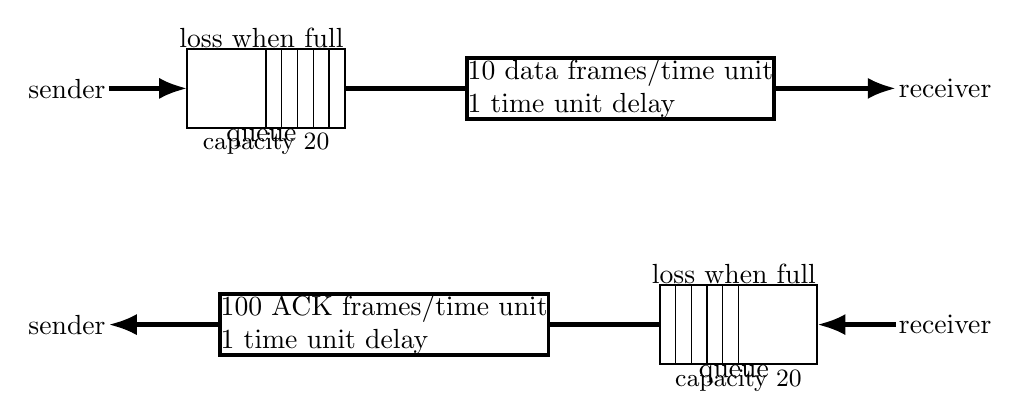
\begin{tikzpicture}
\draw[ultra thick,arrows={-Latex}] (0, 0) node[left] {sender} -- (1, 0);
\draw[thick] (1, -.5) rectangle (3, .5);
\foreach \x in {2,2.2,2.4,2.6,2.8} {
    \draw (\x, -.5) -- (\x, .5);
}
\node[anchor=south,align=center] at (2, .5) {
    loss when full
};
\node[anchor=north,align=center] at (2, -.5) (queue label) {
    queue
};
\node[anchor=north,font=\small] at ([yshift=.2cm]queue label.south) {
    capacity 20
};
\draw[ultra thick,arrows={-Latex}] (3, 0) -- (10, 0) node[right]{receiver}
    node[midway,fill=white,draw=black,very thick,align=left] {
        10 data frames/time unit \\
        1 time unit delay
    };
\begin{scope}[shift={(10, -3)},x=-1cm]
    \draw[ultra thick,arrows={-Latex}] (0, 0) node[right] {receiver} -- (1, 0);
    \draw[thick] (1, -.5) rectangle (3, .5);
    \foreach \x in {2,2.2,2.4,2.6,2.8} {
        \draw (\x, -.5) -- (\x, .5);
    }
    \node[anchor=south,align=center] at (2, .5) {
        loss when full
    };
    \node[anchor=north,align=center] at (2, -.5) (queue label) {
        queue
    };
    \node[anchor=north,font=\small] at ([yshift=.2cm]queue label.south) {
        capacity 20
    };
    \draw[ultra thick,arrows={-Latex}] (3, 0) -- (10, 0) node[left]{sender}
        node[midway,fill=white,draw=black,very thick,align=left] {
            100 ACK frames/time unit \\
            1 time unit delay
        };
\end{scope}
\end{tikzpicture}
\begin{itemize}
\item simulator from upcoming assignment
    \begin{itemize}
    \item command line \texttt{--delay 1 --bandwidth-forward 10 --bandwidth-backward 100 --buffer 30}
    \end{itemize}
\end{itemize}
\end{frame}

\begin{frame}{exercise: forward latency}
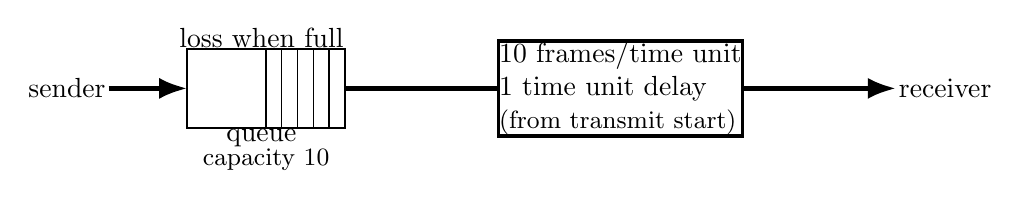
\begin{tikzpicture}
\draw[ultra thick,arrows={-Latex}] (0, 0) node[left] {sender} -- (1, 0);
\draw[thick] (1, -.5) rectangle (3, .5);
\foreach \x in {2,2.2,2.4,2.6,2.8} {
    \draw (\x, -.5) -- (\x, .5);
}
\node[anchor=south,align=center] at (2, .5) {
    loss when full
};
\node[anchor=north,align=center] at (2, -.5) (queue label) {
    queue
};
\node[anchor=north,font=\small] at (queue label.south) {
    capacity 10
};
\draw[ultra thick,arrows={-Latex}] (3, 0) -- (10, 0) node[right]{receiver}
    node[midway,fill=white,draw=black,very thick,align=left] {
        10 frames/time unit \\
        1 time unit delay \\
        \small (from transmit start)
    };
\end{tikzpicture}
\begin{itemize}
\item minimum latency = 1 time unit
\item exercise: maximum latency?
\end{itemize}
\begin{tabular}{lll}
A. 1 time unit & B. 1.1 time unit & C. 1.2 time unit \\
C. 1.4 time unit & D. 1.9 time unit & E. 2.0 time unit \\
F. 2.1 time unit & G. something else \\
\end{tabular}
\end{frame}

\usetikzlibrary{arrows.meta,calc}

\begin{frame}[fragile,label=throughAndWindow]{throughput and window size}
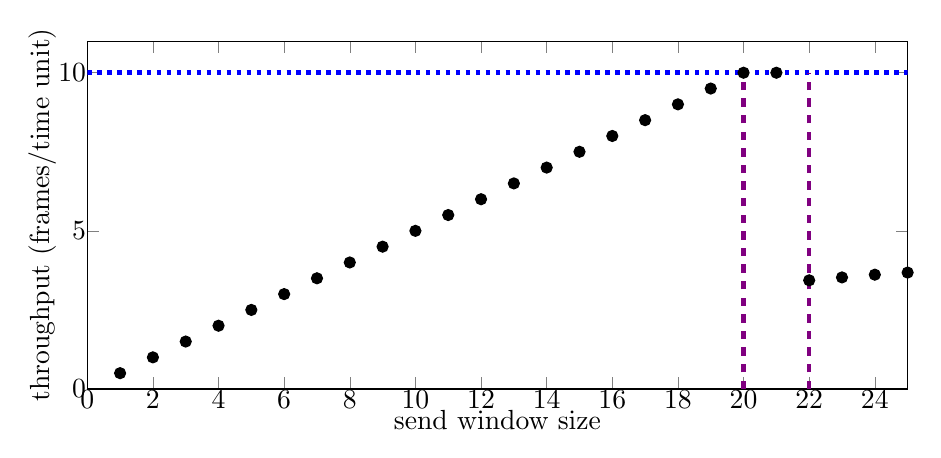
\begin{tikzpicture}
\begin{axis}[width=12cm,height=6cm,
    xlabel=send window size,
    ylabel=throughput (frames/time unit),
    xmin=0,xmax=25,ymin=0]
\addplot[only marks] coordinates {
(1, 0.5000025000125)
(2, 1.0000090000810007)
(3, 1.4999925000374998)
(4, 2.0000280003920055)
(5, 2.500037500562508)
(6, 3.000003000003)
(7, 3.5000035000035)
(8, 4.000048000576006)
(9, 4.499842505512307)
(10, 5.000025000125)
(11, 5.499975250111374)
(12, 5.99977200866367)
(13, 6.499710762871052)
(14, 6.999811005102861)
(15, 7.4996812635462975)
(16, 7.999680012799485)
(17, 8.499426288725509)
(18, 8.999361045365776)
(19, 9.499202067026369)
(20, 9.999100080971061)
(21, 9.999100080973866)
(22, 3.435635094325549)
(23, 3.5274986154570636)
(24, 3.613708966335035)
(25, 3.6808686850100703)
(26, 3.753260645186032)
(27, 3.8487443471573166)
(28, 3.925956461143474)
};
\addplot[blue,dotted,ultra thick,domain=0:25] {10};
    \draw[violet,dashed,ultra thick] (axis cs:20,0) -- (axis cs:20, 10)
     coordinate (empty queue mark);
    \draw[violet,dashed,ultra thick] (axis cs:21.99,0) -- (axis cs:21.99, 10)
     coordinate (full queue mark);
\end{axis}
\end{tikzpicture}
\end{frame}

\usetikzlibrary{arrows.meta,calc}

\begin{frame}{simple network model}
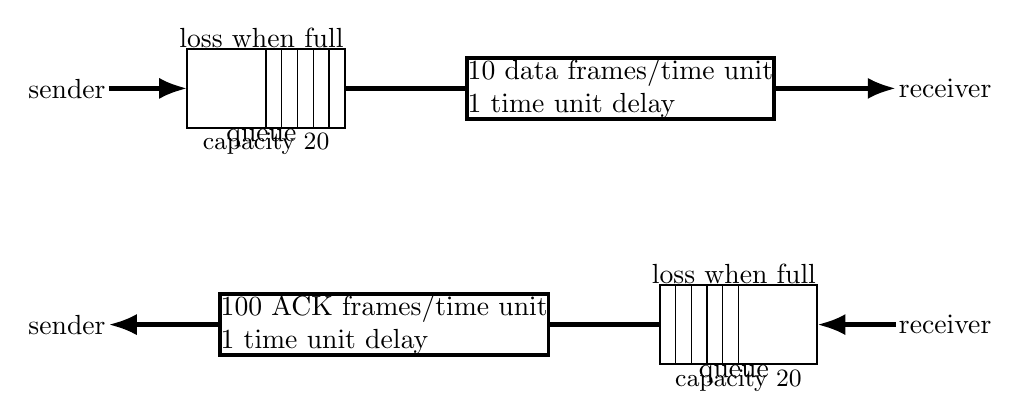
\begin{tikzpicture}
\draw[ultra thick,arrows={-Latex}] (0, 0) node[left] {sender} -- (1, 0);
\draw[thick] (1, -.5) rectangle (3, .5);
\foreach \x in {2,2.2,2.4,2.6,2.8} {
    \draw (\x, -.5) -- (\x, .5);
}
\node[anchor=south,align=center] at (2, .5) {
    loss when full
};
\node[anchor=north,align=center] at (2, -.5) (queue label) {
    queue
};
\node[anchor=north,font=\small] at ([yshift=.2cm]queue label.south) {
    capacity 20
};
\draw[ultra thick,arrows={-Latex}] (3, 0) -- (10, 0) node[right]{receiver}
    node[midway,fill=white,draw=black,very thick,align=left] {
        10 data frames/time unit \\
        1 time unit delay
    };
\begin{scope}[shift={(10, -3)},x=-1cm]
    \draw[ultra thick,arrows={-Latex}] (0, 0) node[right] {receiver} -- (1, 0);
    \draw[thick] (1, -.5) rectangle (3, .5);
    \foreach \x in {2,2.2,2.4,2.6,2.8} {
        \draw (\x, -.5) -- (\x, .5);
    }
    \node[anchor=south,align=center] at (2, .5) {
        loss when full
    };
    \node[anchor=north,align=center] at (2, -.5) (queue label) {
        queue
    };
    \node[anchor=north,font=\small] at ([yshift=.2cm]queue label.south) {
        capacity 20
    };
    \draw[ultra thick,arrows={-Latex}] (3, 0) -- (10, 0) node[left]{sender}
        node[midway,fill=white,draw=black,very thick,align=left] {
            100 ACK frames/time unit \\
            1 time unit delay
        };
\end{scope}
\end{tikzpicture}
\begin{itemize}
\item simulator from upcoming assignment
    \begin{itemize}
    \item command line \texttt{--delay 1 --bandwidth-forward 10 --bandwidth-backward 100 --buffer 30}
    \end{itemize}
\end{itemize}
\end{frame}

\begin{frame}{exercise: forward latency}
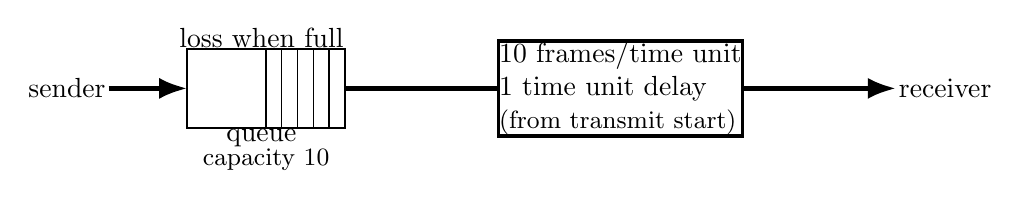
\begin{tikzpicture}
\draw[ultra thick,arrows={-Latex}] (0, 0) node[left] {sender} -- (1, 0);
\draw[thick] (1, -.5) rectangle (3, .5);
\foreach \x in {2,2.2,2.4,2.6,2.8} {
    \draw (\x, -.5) -- (\x, .5);
}
\node[anchor=south,align=center] at (2, .5) {
    loss when full
};
\node[anchor=north,align=center] at (2, -.5) (queue label) {
    queue
};
\node[anchor=north,font=\small] at (queue label.south) {
    capacity 10
};
\draw[ultra thick,arrows={-Latex}] (3, 0) -- (10, 0) node[right]{receiver}
    node[midway,fill=white,draw=black,very thick,align=left] {
        10 frames/time unit \\
        1 time unit delay \\
        \small (from transmit start)
    };
\end{tikzpicture}
\begin{itemize}
\item minimum latency = 1 time unit
\item exercise: maximum latency?
\end{itemize}
\begin{tabular}{lll}
A. 1 time unit & B. 1.1 time unit & C. 1.2 time unit \\
C. 1.4 time unit & D. 1.9 time unit & E. 2.0 time unit \\
F. 2.1 time unit & G. something else \\
\end{tabular}
\end{frame}

\begin{frame}[fragile,label=throughAndWindow]{throughput and window size}
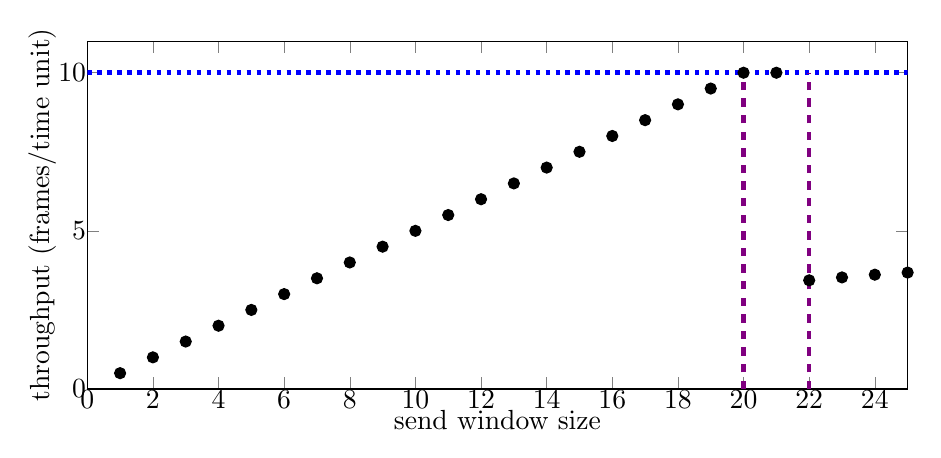
\begin{tikzpicture}
\begin{axis}[width=12cm,height=6cm,
    xlabel=send window size,
    ylabel=throughput (frames/time unit),
    xmin=0,xmax=25,ymin=0]
\addplot[only marks] coordinates {
(1, 0.5000025000125)
(2, 1.0000090000810007)
(3, 1.4999925000374998)
(4, 2.0000280003920055)
(5, 2.500037500562508)
(6, 3.000003000003)
(7, 3.5000035000035)
(8, 4.000048000576006)
(9, 4.499842505512307)
(10, 5.000025000125)
(11, 5.499975250111374)
(12, 5.99977200866367)
(13, 6.499710762871052)
(14, 6.999811005102861)
(15, 7.4996812635462975)
(16, 7.999680012799485)
(17, 8.499426288725509)
(18, 8.999361045365776)
(19, 9.499202067026369)
(20, 9.999100080971061)
(21, 9.999100080973866)
(22, 3.435635094325549)
(23, 3.5274986154570636)
(24, 3.613708966335035)
(25, 3.6808686850100703)
(26, 3.753260645186032)
(27, 3.8487443471573166)
(28, 3.925956461143474)
};
\addplot[blue,dotted,ultra thick,domain=0:25] {10};
    \draw[violet,dashed,ultra thick] (axis cs:20,0) -- (axis cs:20, 10)
     coordinate (empty queue mark);
    \draw[violet,dashed,ultra thick] (axis cs:21.99,0) -- (axis cs:21.99, 10)
     coordinate (full queue mark);
\end{axis}
\end{tikzpicture}
\end{frame}

\begin{frame}[fragile,label=transitTime]{packet transit time}
\begin{tikzpicture}
\draw[ultra thick,arrows={-Latex}] (0, 0) node[left] {sender} -- (1, 0);
\draw[thick] (1, -.5) rectangle (3, .5);
\foreach \x in {2,2.2,2.4,2.6,2.8} {
    \draw (\x, -.5) -- (\x, .5);
}
\node[anchor=south,align=center] at (2, .5) {
    loss when full
};
\node[anchor=north,align=center] at (2, -.5) (queue label) {
    queue
};
\node[anchor=north,font=\fontsize{9}{10}\selectfont] at ([yshift=.3cm]queue label.south) {
    capacity 20
};
\draw[ultra thick,arrows={-Latex}] (3, 0) -- (12, 0) node[right]{receiver}
    node[midway,fill=white,draw=black,very thick,align=left] {
        10 data frames/time unit \\
        1 time unit delay
    }
    node[visible on=<1-3>,ultra thick,pos=0,draw=black,fill=white,font=\tiny,below=.5cm] (data-main) {data};
    \begin{visibleenv}<2->
    \draw[red,-Latex,very thick] (data-main.east) -- (data-main.west -| 13, 0) coordinate (end send)
        node[midway,below,font=\small] {1 time unit (sender to receiver)};
    \end{visibleenv}
\begin{scope}[shift={(12, -4)},x=-1cm]
    \draw[ultra thick,arrows={-Latex}] (0, 0) node[right] {receiver} -- (1, 0);
    \draw[thick] (1, -.5) rectangle (3, .5);
    \foreach \x in {2,2.2,2.4,2.6,2.8} {
        \draw (\x, -.5) -- (\x, .5);
    }
    \node[anchor=south,align=center] at (2, .5) {
        loss when full
    };
    \node[anchor=north,align=center] at (2, -.5) (queue label) {
        queue
    };
    \node[anchor=north,font=\small] at ([yshift=.2cm]queue label.south) {
        capacity 20
    };
    \draw[ultra thick,arrows={-Latex}] (3, 0) -- (12, 0) node[left]{sender}
        node[midway,fill=white,draw=black,very thick,align=left] {
            100 ACK frames/time unit \\
            1 time unit delay
        }
        node[visible on=<2->,pos=0,draw=red,fill=white,font=\tiny,below=.5cm,align=center,inner sep=0.5mm] 
            (ack-start) {a\\c\\k};
    \begin{visibleenv}<2->
        \draw[dotted,red,-Latex,very thick] (end send) |- (ack-start.east);
        \draw[red,-Latex,very thick] (ack-start.west) -- (ack-start.west -| 12, 0) node[midway,below,font=\small] { + 1 time unit (receiver to sender)};
    \end{visibleenv}
\end{scope}
\begin{visibleenv}<3>
\node[draw=red,fill=white,ultra thick,align=left] at (6, -2.5) {
    takes 1 + 1 time units to send message + receive ack \\
    goal: keep sending stuff while waiting
};
\end{visibleenv}
\end{tikzpicture}
\end{frame}

\begin{frame}{filling the pipe}
    \begin{itemize}
    \item round-trip time of 2 time units
        \begin{itemize}
        \item from send data to receive ACK (assuming no queuing delay)
        \end{itemize}
    \item can send 10 data frames per time unit
    \item = can send 20 data frames while waiting for ACK
    \vspace{.5cm}
    \item<2> \myemph{``bandwidth-delay product''}
        \begin{itemize}
        \item 10/time unit (banwidth) times 2 time unit (RTT = delay)
        \end{itemize}
    \end{itemize}
\end{frame}

\begin{frame}[fragile,label=throughAndWindow]{throughput and window size (detail)}
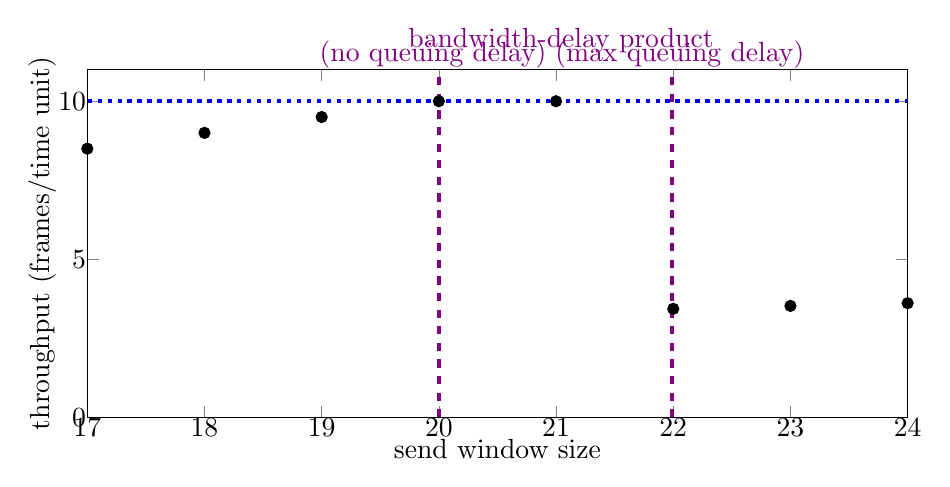
\begin{tikzpicture}
\begin{axis}[width=12cm,height=6cm,
    xlabel=send window size,
    ylabel=throughput (frames/time unit),
    xmin=17,xmax=24,ymin=0]
\addplot[only marks] coordinates {
(1, 0.5000025000125)
(2, 1.0000090000810007)
(3, 1.4999925000374998)
(4, 2.0000280003920055)
(5, 2.500037500562508)
(6, 3.000003000003)
(7, 3.5000035000035)
(8, 4.000048000576006)
(9, 4.499842505512307)
(10, 5.000025000125)
(11, 5.499975250111374)
(12, 5.99977200866367)
(13, 6.499710762871052)
(14, 6.999811005102861)
(15, 7.4996812635462975)
(16, 7.999680012799485)
(17, 8.499426288725509)
(18, 8.999361045365776)
(19, 9.499202067026369)
(20, 9.999100080971061)
(21, 9.999100080973866)
(22, 3.435635094325549)
(23, 3.5274986154570636)
(24, 3.613708966335035)
(25, 3.6808686850100703)
(26, 3.753260645186032)
(27, 3.8487443471573166)
(28, 3.925956461143474)
};
\addplot[blue,dotted,ultra thick,domain=0:25] {10};
    \draw[violet,dashed,ultra thick] (axis cs:20,0) -- (axis cs:20, 11)
     coordinate (empty queue mark);
    \draw[violet,dashed,ultra thick] (axis cs:21.99,0) -- (axis cs:21.99, 11)
     coordinate (full queue mark);
\end{axis}
\node[violet,anchor=south east,align=right] (nq) at ([xshift=1.5cm]empty queue mark) {
    (no queuing delay)
};
\node[violet,anchor=south west,align=left] (mq) at ([xshift=-1.5cm]full queue mark) {
    (max queuing delay)
};
\node[violet,anchor=south] at ($(nq)!0.5!(mq)$) {bandwidth-delay product};
\end{tikzpicture}
\end{frame}


\begin{frame}[fragile,label=fullPipe]{filling the pipe}
\begin{tikzpicture}
\draw[ultra thick,arrows={-Latex}] (0, 0) node[left] {sender} -- (1, 0);
\draw[thick] (1, -.5) rectangle (3, .5);
\foreach \x in {2,2.2,2.4,2.6,2.8} {
    \draw (\x, -.5) -- (\x, .5);
}
\node[anchor=south,align=center] at (2, .5) {
    loss when full
};
\node[anchor=north,align=center] at (2, -.5) (queue label) {
    queue
};
\node[anchor=north,font=\fontsize{9}{10}\selectfont] at ([yshift=.3cm]queue label.south) {
    capacity 20
};
\draw[ultra thick,arrows={-Latex}] (3, 0) -- (12, 0) node[right]{receiver}
    node[midway,fill=white,draw=black,very thick,align=left] {
        10 data frames/time unit \\
        1 time unit delay
    }
    \foreach \x in {0,1,2,3,4,5,6,7,8,9} {
        node[visible on=<3->,pos=\x*.1+0.05,draw=black,fill=white,font=\tiny,below=.5cm] (data-\x) {data}
    };
    \begin{visibleenv}<3->
    \draw[red,Latex-Latex] ([yshift=-.1cm]data-0.south west) -- ([yshift=-.1cm]data-1.south west)
        node[below,font=\small] {0.1 time unit};
    \end{visibleenv}
\begin{scope}[shift={(12, -4)},x=-1cm]
    \draw[ultra thick,arrows={-Latex}] (0, 0) node[right] {receiver} -- (1, 0);
    \draw[thick] (1, -.5) rectangle (3, .5);
    \foreach \x in {2,2.2,2.4,2.6,2.8} {
        \draw (\x, -.5) -- (\x, .5);
    }
    \node[anchor=south,align=center] at (2, .5) {
        loss when full
    };
    \node[anchor=north,align=center] at (2, -.5) (queue label) {
        queue
    };
    \node[anchor=north,font=\small] at ([yshift=.2cm]queue label.south) {
        capacity 20
    };
    \draw[ultra thick,arrows={-Latex}] (3, 0) -- (12, 0) node[left]{sender}
        node[midway,fill=white,draw=black,very thick,align=left] {
            100 ACK frames/time unit \\
            1 time unit delay
        }
        \foreach \x in {0,1,2,3,4,5,6,7,8,9} {
            node[visible on=<3->,pos=\x*.1+0.05,draw=black,fill=white,font=\tiny,below=.5cm,align=center,inner sep=0.5mm] {a\\c\\k}
        };
\end{scope}
\end{tikzpicture}
\end{frame}



\begin{frame}[fragile,label=throughAndWindow]{throughput and window size (detail)}
\begin{tikzpicture}
\begin{axis}[width=12cm,height=6cm,
    xlabel=send window size,
    ylabel=throughput (frames/time unit),
    xmin=17,xmax=24,ymin=0]
\addplot[only marks] coordinates {
(1, 0.5000025000125)
(2, 1.0000090000810007)
(3, 1.4999925000374998)
(4, 2.0000280003920055)
(5, 2.500037500562508)
(6, 3.000003000003)
(7, 3.5000035000035)
(8, 4.000048000576006)
(9, 4.499842505512307)
(10, 5.000025000125)
(11, 5.499975250111374)
(12, 5.99977200866367)
(13, 6.499710762871052)
(14, 6.999811005102861)
(15, 7.4996812635462975)
(16, 7.999680012799485)
(17, 8.499426288725509)
(18, 8.999361045365776)
(19, 9.499202067026369)
(20, 9.999100080971061)
(21, 9.999100080973866)
(22, 3.435635094325549)
(23, 3.5274986154570636)
(24, 3.613708966335035)
(25, 3.6808686850100703)
(26, 3.753260645186032)
(27, 3.8487443471573166)
(28, 3.925956461143474)
};
\addplot[blue,dotted,ultra thick,domain=0:25] {10};
    \draw[violet,dashed,ultra thick] (axis cs:20,0) -- (axis cs:20, 11)
     coordinate (empty queue mark);
    %\draw[violet,dashed,ultra thick] (axis cs:21.99,0) -- (axis cs:21.99, 11)
    % coordinate (full queue mark);
\end{axis}
\node[violet,anchor=south east,align=right] (nq) at ([xshift=1.5cm]empty queue mark) {
    (no queuing delay)
};
\node[violet,anchor=south west,align=left] (mq) at ([xshift=-1.5cm]full queue mark) {
    (max useful queuing delay)
};
\node[violet,anchor=south] at (nq) {bandwidth-delay product\\w/o queuing delay};
\end{tikzpicture}
\end{frame}


\begin{frame}[fragile,label=fullPipe]{filling the pipe}
\begin{tikzpicture}
\draw[ultra thick,arrows={-Latex}] (0, 0) node[left] {sender} -- (1, 0);
\draw[thick] (1, -.5) rectangle (3, .5);
\foreach \x in {2,2.2,2.4,2.6,2.8} {
    \draw (\x, -.5) -- (\x, .5);
}
\node[anchor=south,align=center] at (2, .5) {
    loss when full
};
\node[anchor=north,align=center] at (2, -.5) (queue label) {
    queue
};
\node[anchor=north,font=\fontsize{9}{10}\selectfont] at ([yshift=.3cm]queue label.south) {
    capacity 20
};
\draw[ultra thick,arrows={-Latex}] (3, 0) -- (12, 0) node[right]{receiver}
    node[midway,fill=white,draw=black,very thick,align=left] {
        10 data frames/time unit \\
        1 time unit delay
    }
    \foreach \x in {0,1,2,3,4,5,6,7,8,9} {
        node[visible on=<3->,pos=\x*.1+0.05,draw=black,fill=white,font=\tiny,below=.5cm] (data-\x) {data}
    };
    \begin{visibleenv}<3->
    \draw[red,Latex-Latex] ([yshift=-.1cm]data-0.south west) -- ([yshift=-.1cm]data-1.south west)
        node[below,font=\small] {0.1 time unit};
    \end{visibleenv}
\begin{scope}[shift={(12, -4)},x=-1cm]
    \draw[ultra thick,arrows={-Latex}] (0, 0) node[right] {receiver} -- (1, 0);
    \draw[thick] (1, -.5) rectangle (3, .5);
    \foreach \x in {2,2.2,2.4,2.6,2.8} {
        \draw (\x, -.5) -- (\x, .5);
    }
    \node[anchor=south,align=center] at (2, .5) {
        loss when full
    };
    \node[anchor=north,align=center] at (2, -.5) (queue label) {
        queue
    };
    \node[anchor=north,font=\small] at ([yshift=.2cm]queue label.south) {
        capacity 20
    };
    \draw[ultra thick,arrows={-Latex}] (3, 0) -- (12, 0) node[left]{sender}
        node[midway,fill=white,draw=black,very thick,align=left] {
            100 ACK frames/time unit \\
            1 time unit delay
        }
        \foreach \x in {0,1,2,3,4,5,6,7,8,9} {
            node[visible on=<3->,pos=\x*.1+0.05,draw=black,fill=white,font=\tiny,below=.5cm,align=center,inner sep=0.5mm] {a\\c\\k}
        };
\end{scope}
\end{tikzpicture}
\end{frame}

\begin{frame}{on bursts}
    \begin{itemize}
    \item max possible queuing delay suggests window size of 30
        \begin{itemize}
        \item approx. 3 time units times 10
        \end{itemize}
    \item problem: ``bursts'' temporarily exceed queue size
    \vspace{.5cm}
    \item achievable average queue size not that high
    \item sender could moderate by ``pacing'' packets
    \end{itemize}
\end{frame}


\subsection{problems solved}
\begin{frame}{sliding windows solve\ldots}
    \begin{itemize}
    \item reliability on unrelaible link
    \item \textit{congestion control}
        \begin{itemize}
        \item keep network from being overloaded
        \item \ldots by having window sizes set correctly
        \end{itemize}
    \item \textit{flow control}
        \begin{itemize}
        \item keep sender from getting too far ahead of sender
        \item \ldots by having window sizes set correctly
        \end{itemize}
    \end{itemize}
\end{frame}


\subsection{sequence number wraparound}
\usetikzlibrary{arrows.meta, calc, fit, matrix, patterns, shapes.misc}

\providecommand{\computer}{%
    
\includegraphics[width=1cm]{../common/Noun_project_216.pdf}
}
\providecommand{\switch}{%
    
\includegraphics[width=0.9cm]{../common/fig-switch.pdf}
}
\providecommand{\bigswitch}{%
    
\includegraphics[width=1.4cm]{../common/fig-switch.pdf}
}
\providecommand{\router}{%
    
\includegraphics[width=0.9cm]{../common/fig-router.pdf}
}


\begin{frame}{sequence number wraparound}
    \begin{itemize}
    \item protocol so far requires arbitrarily large sequence numbers
        \begin{itemize}
        \item doing $<$ and $>$ checks on sequence number, so they need to increase
        \end{itemize}
    \item would like to use smaller sequence numbers
        \begin{itemize}
        \item think: transferring multi-gigabyte file
        \end{itemize}
    \item question: what goes wrong when we reuse sequeunce numbers?
    \end{itemize}
\end{frame}

\begin{frame}{sender/receiver desync: missing ACKs}
\begin{tikzpicture}
\tikzset{
    seqlist/.style={tight matrix,nodes={text width=.8cm,minimum height=.8cm},column sep=.6mm},
    dots/.style={draw=none,execute at begin node=\ldots,anchor=center,font=\huge,text width=1cm,align=center},
    region mark/.style={very thick,decorate,decoration={brace,mirror}},
    region mark label/.style={midway,below,align=center},
    verified/.style={pattern color=black!30,pattern=checkerboard},
    ack sent not recvd/.style={fill=blue!60},
    unsent ready/.style={pattern color=yellow!30!black,pattern=checkerboard},
    unsent/.style={pattern=crosshatch dots,pattern color=violet!70},
}
\begin{scope}[name prefix=s-]
    \matrix[seqlist] (window) {
        |[dots,alias=window-start]| ~ \& |[alias=after-window-start,verified,alias=LAR]| ~ \&
        |[ack sent not recvd,alias=after LAR]| ~ \& |[ack sent not recvd]| ~ \& |[ack sent not recvd]| ~ \& 
        |[ack sent not recvd,alias=LFS]| ~ \& 
        |[alias=after LFS,unsent]| ~ \& |[unsent,alias=before-window-end]| ~  \&
        |[unsent]| ~  \&
        |[unsent]| ~  \&
        |[unsent]| ~  \&
        |[unsent,alias=before-window-end]| ~  \&
        \& |[alias=window-end,dots]| \\
    };
    \node[anchor=east] at (window-start.west) {sender};
    \draw[thick,Latex-] (LAR.north) -- ++(0,.5) node[above,align=center] (LAR label) {(LAR)\\last ACK recv'd};
    \draw[thick,Latex-] (LFS.north) -- ++(0,.5) node[above,align=center] (LFS label) {(LFS)\\last frame sent};
\end{scope}
\begin{scope}[name prefix=r-,yshift=-3cm]
    \matrix[seqlist] (window) {
        |[dots,alias=window-start]| ~ \& |[alias=after-window-start,verified]| ~ \& 
        |[alias=after LAR,ack sent not recvd]| ~ \& |[ack sent not recvd]| ~ \& 
        |[ack sent not recvd]| ~ \& |[alias=LFR,ack sent not recvd]| ~ \&
        |[unsent ready,alias=after LFR]| ~ \& |[unsent ready,alias=after after LFR]| ~ \&
        |[unsent ready]| ~ \& |[unsent ready,alias=LAF]| ~ \& 
        |[alias=after LAF,unsent]| ~ \& |[unsent,alias=before-window-end]| ~ \& |[alias=window-end,dots]| \\
    };
    \node[anchor=east] at (window-start.west) {receiver};
    \draw[thick,Latex-] (LFR.north) -- ++(0,.5) node[above,align=center] {(LFR)\\last frame recv'd*};
    \draw[thick,Latex-] (LAF.north) -- ++(0,.5) node[above,align=center] {(LAF)\\last accepted frame};
    \draw[region mark] ([yshift=-.1cm]after LAR.south west) -- ([yshift=-.1cm]LFR.south east)
        node[region mark label] {resent if \\ ACK lost};
    \draw[region mark] ([yshift=-.1cm]after LFR.south west) -- ([yshift=-.1cm]LAF.south east)
        node[region mark label] {expected if \\ ACK not lost};
\end{scope}
\begin{visibleenv}<2->
\node[draw=red,ultra thick,fit=(s-after LAR) (r-LAF),label={[red,align=left,fill=white,fill opacity=0.95]west:need unique \\ numbers for all these}] {};
\end{visibleenv}
\begin{visibleenv}<3->
\foreach \x/\lbl in {2/4,3/5,4/6,5/7,6/0,7/1,8/2,9/3,10/4,11/5,12/6,13/7} {
    \node[fill=white,font=\small,text=red,circle,draw=red,ultra thick,anchor=south west,inner sep=0.1mm] at ([xshift=\x * .935cm - 0.4cm]s-window-start.north west) {\lbl};
}
\end{visibleenv}
\end{tikzpicture}
\end{frame}

\begin{frame}{wraparound}
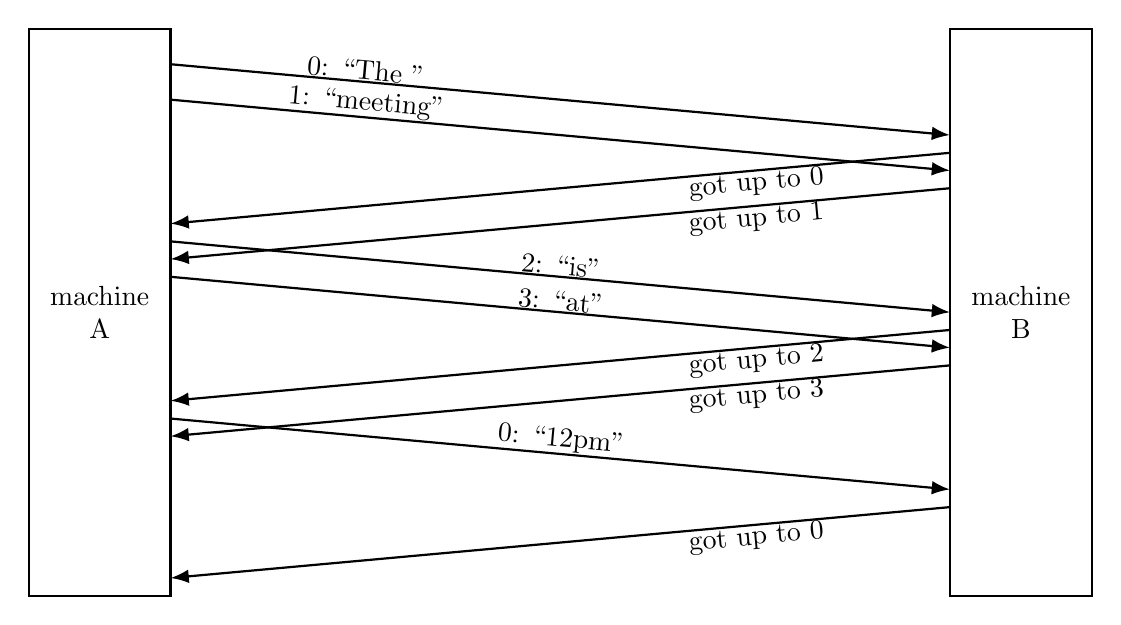
\begin{tikzpicture}
\tikzset{
    box/.style={thick},
    message/.style={draw,thick,-Latex},
    failure/.style={draw,ultra thick,red,cross out,minimum width=1cm,minimum height=1cm},
    every node/.style={inner sep=0.1mm},
}
\begin{scope}[xshift=1cm,x=0.9cm,y=0.9cm]
\draw[box] (0, 0) rectangle ++(2, -8) 
    node[midway,align=center] {machine\\A};
\draw[box] (13, 0) rectangle ++(2, -8) 
    node[midway,align=center] {machine\\B};
\draw[message] (2, -0.5) -- (13, -1.5) node[pos=0.25,above,sloped] {\myemph{0}: ``The ''};
\draw[message] (13, -1.75) -- (2, -2.75) node[pos=0.25,sloped,below] {got up to \myemph{0}};
\draw[message] (2, -1) -- (13, -2) node[pos=0.25, above, sloped] {\myemph{1}: ``meeting''};
\draw[message] (13, -2.25) -- (2, -3.25) node[pos=0.25, sloped,below] {got up to \myemph{1}};

% in response to got 0
\draw[message] (2, -3) -- (13, -4) node[pos=0.5, above, sloped] {\myemph{2}: ``is''};
\draw[message] (13, -4.25) -- (2, -5.25) node[pos=0.25, sloped,below] {got up to \myemph{2}};
% in response to got 1
\draw[message] (2, -3.5) -- (13, -4.5) node[pos=0.5, above, sloped] {\myemph{3}: ``at''};
\draw[message] (13, -4.75) -- (2, -5.75) node[pos=0.25, sloped,below] {got up to \myemph{3}};

% in response to got 2
\draw[message] (2, -5.5) -- (13, -6.5) node[pos=0.5, above, sloped] {\myemph{0}: ``12pm''};
\draw[message] (13, -6.75) -- (2, -7.75) node[pos=0.25, sloped,below] {got up to \myemph{0}};
\end{scope}
\end{tikzpicture}
\end{frame}

\begin{frame}{loss and resend?}
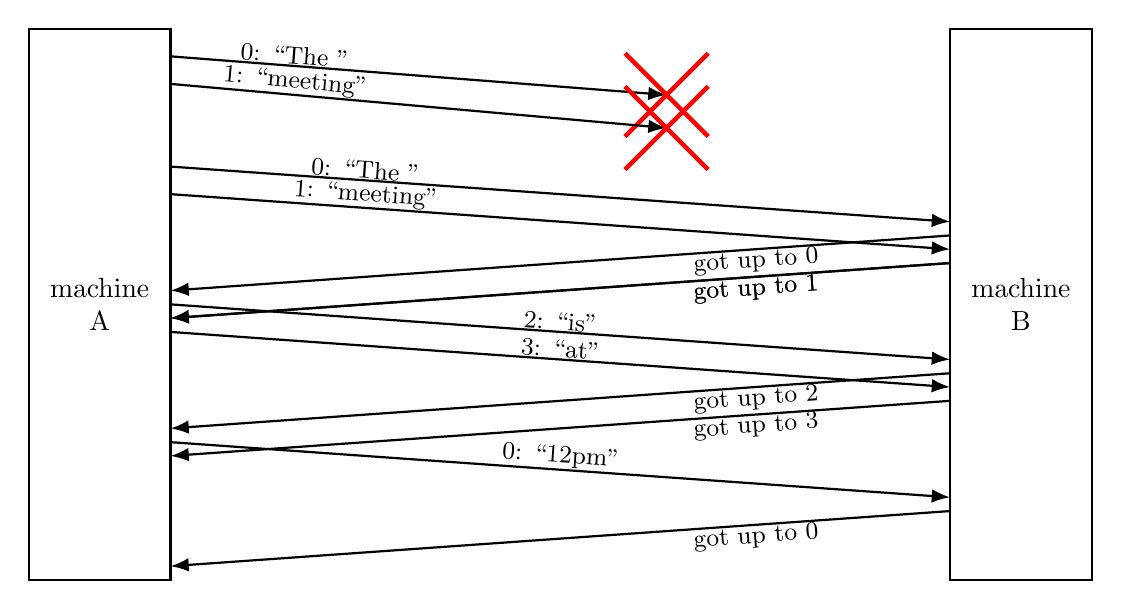
\begin{tikzpicture}
\tikzset{
    box/.style={thick},
    message/.style={draw,thick,-Latex,font=\small},
    failure/.style={draw,ultra thick,red,cross out,minimum width=1cm,minimum height=1cm},
    every node/.style={inner sep=0.1mm},
}
\begin{scope}[xshift=1cm,x=0.9cm,y=0.7cm]
\draw[box] (0, 2) rectangle ++(2, -10) 
    node[midway,align=center] {machine\\A};
\draw[box] (13, 2) rectangle ++(2, -10) 
    node[midway,align=center] {machine\\B};
\draw[message] (2, 2-0.5) -- (9, 2-1.2) node[pos=0.25,above,sloped] {\myemph{0}: ``The ''} node[failure] {};
\draw[message] (2, 2-1) -- (9, 2-1.8) node[pos=0.25, above, sloped] {\myemph{1}: ``meeting''} node[failure] {};
\draw[message] (13, -2.25) -- (2, -3.25) node[pos=0.25, sloped,below] {got up to \myemph{1}};
\draw[message] (2, -0.5) -- (13, -1.5) node[pos=0.25,above,sloped] {\myemph{0}: ``The ''};
\draw[message] (13, -1.75) -- (2, -2.75) node[pos=0.25,sloped,below] {got up to \myemph{0}};
\draw[message] (2, -1) -- (13, -2) node[pos=0.25, above, sloped] {\myemph{1}: ``meeting''};
\draw[message] (13, -2.25) -- (2, -3.25) node[pos=0.25, sloped,below] {got up to \myemph{1}};

% in response to got 0
\draw[message] (2, -3) -- (13, -4) node[pos=0.5, above, sloped] {\myemph{2}: ``is''};
\draw[message] (13, -4.25) -- (2, -5.25) node[pos=0.25, sloped,below] {got up to \myemph{2}};
% in response to got 1
\draw[message] (2, -3.5) -- (13, -4.5) node[pos=0.5, above, sloped] {\myemph{3}: ``at''};
\draw[message] (13, -4.75) -- (2, -5.75) node[pos=0.25, sloped,below] {got up to \myemph{3}};

% in response to got 2
\draw[message] (2, -5.5) -- (13, -6.5) node[pos=0.5, above, sloped] {\myemph{0}: ``12pm''};
\draw[message] (13, -6.75) -- (2, -7.75) node[pos=0.25, sloped,below] {got up to \myemph{0}};
\end{scope}
\end{tikzpicture}
\end{frame}

\begin{frame}{very bad reordering}
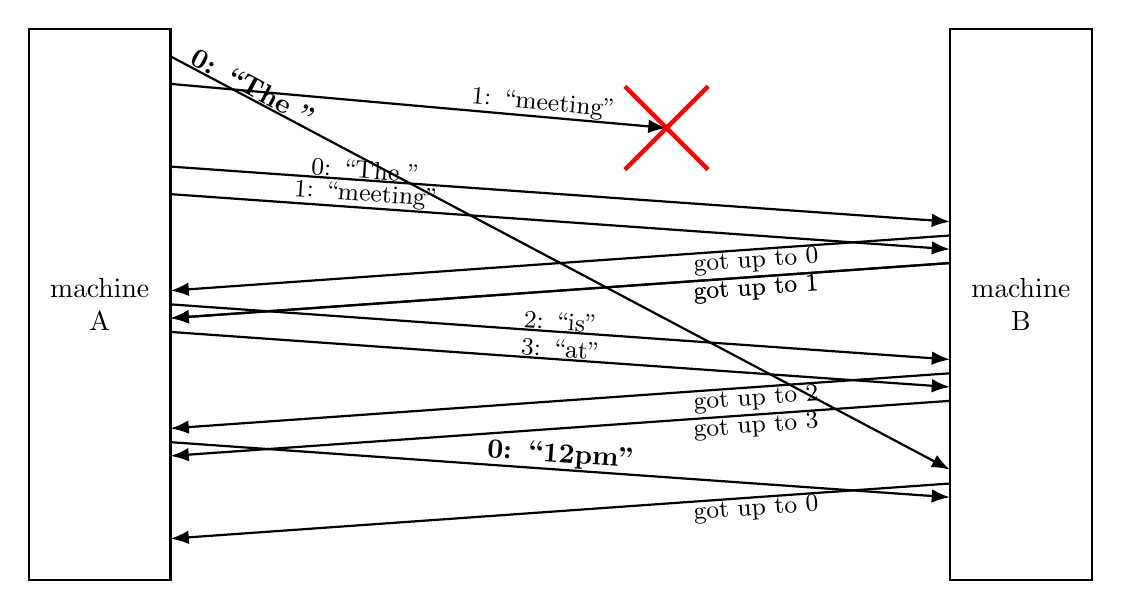
\begin{tikzpicture}
\tikzset{
    box/.style={thick},
    message/.style={draw,thick,-Latex,font=\small},
    failure/.style={draw,ultra thick,red,cross out,minimum width=1cm,minimum height=1cm},
    every node/.style={inner sep=0.1mm},
}
\begin{scope}[xshift=1cm,x=0.9cm,y=0.7cm]
\draw[box] (0, 2) rectangle ++(2, -10) 
    node[midway,align=center] {machine\\A};
\draw[box] (13, 2) rectangle ++(2, -10) 
    node[midway,align=center] {machine\\B};
\draw[message] (2, 2-0.5) -- (13, -6) node[pos=0.1,above,sloped,font=\bfseries] {\myemph{0}: ``The ''};
\draw[message] (2, 2-1) -- (9, 2-1.8) node[pos=0.75, above, sloped] {\myemph{1}: ``meeting''} node[failure] {};
\draw[message] (13, -2.25) -- (2, -3.25) node[pos=0.25, sloped,below] {got up to \myemph{1}};
\draw[message] (2, -0.5) -- (13, -1.5) node[pos=0.25,above,sloped] {\myemph{0}: ``The ''};
\draw[message] (13, -1.75) -- (2, -2.75) node[pos=0.25,sloped,below] {got up to \myemph{0}};
\draw[message] (2, -1) -- (13, -2) node[pos=0.25, above, sloped] {\myemph{1}: ``meeting''};
\draw[message] (13, -2.25) -- (2, -3.25) node[pos=0.25, sloped,below] {got up to \myemph{1}};

% in response to got 0
\draw[message] (2, -3) -- (13, -4) node[pos=0.5, above, sloped] {\myemph{2}: ``is''};
\draw[message] (13, -4.25) -- (2, -5.25) node[pos=0.25, sloped,below] {got up to \myemph{2}};
% in response to got 1
\draw[message] (2, -3.5) -- (13, -4.5) node[pos=0.5, above, sloped] {\myemph{3}: ``at''};
\draw[message] (13, -4.75) -- (2, -5.75) node[pos=0.25, sloped,below] {got up to \myemph{3}};

% in response to got 2
\draw[message] (2, -5.5) -- (13, -6.5) node[pos=0.5, above, sloped,font=\bfseries] {\myemph{0}: ``12pm''};
% in response to BOGUS got 0
\draw[message] (13, -6.25) -- (2, -7.25) node[pos=0.25, sloped,below] {got up to \myemph{0}};
\end{scope}
\end{tikzpicture}
\end{frame}

\begin{frame}{possible reason}
\begin{tikzpicture}
\tikzset{
    connect one/.style={draw,very thick,Latex-Latex},
    computer/.style={inner sep=0mm,outer sep=0mm,execute at begin node={\computer}},
    switch/.style={inner sep=0mm,outer sep=0mm,execute at begin node={\switch}},
    router/.style={inner sep=0mm,outer sep=0mm,execute at begin node={\router}},
    big switch/.style={inner sep=0mm,outer sep=0mm,execute at begin node={\bigswitch}},
    packet/.style={minimum width=.4cm,minimum height=0.2cm,inner sep=0mm,outer sep=0mm,draw},
    packet lg/.style={minimum width=.6cm,minimum height=0.2cm,inner sep=0mm,outer sep=0mm,draw},
}
\node[computer] (start) at (0,0) {};
\node[computer] (end)  at (13,0) {};
\node[router] (pre1) at (3, 3) {};
\node[router] (pre2) at (4, .5) {};
\node[router] (pre3) at (5, 3) {};
\node[router] (A) at (6, 1) {};
\node[router] (B) at (7, -1) {};
\node[router] (C) at (8, 3) {};
\node[router] (D) at (11, 0) {};
\
\node[router] (E) at (7.5, -2) {};
\foreach \x/\y in {start/pre1,pre1/pre2,pre2/pre3,pre3/A,A/B,B/C,C/D,D/end,start/E,E/end} {
    \draw[connect one] (\x) -- (\y);
}
\node[font=\small,draw,fill=white] at ($(C)!0.5!(D)$) {\myemph{0}: ``The ''};
\node[font=\small,draw,fill=white] at ($(E)!0.7!(start)$) {\myemph{0}: ``12pm''};
\end{tikzpicture}
\end{frame}




\section{TCP example}

\subsection{TCP segment format}
\usetikzlibrary{patterns}
\begin{frame}{TCP}
    \begin{itemize}
    \item transmission control protocol (TCP)
    \item implements reliable streams of bytes
    \item similar mechanism to what we've described
    \end{itemize}
\end{frame}

\begin{frame}{TCP extras/differences}
    \begin{itemize}
    \item bidirectional ---
        \begin{itemize}
        \item separate sequence numbers in each direction
        \item can combine data (from A to B) with acknowledgment (from B to A)
        \end{itemize}
    \item sequence numbers are byte numbers ---
        \begin{itemize}
        \item can retransmit data in different sized packets
        \item sequence numbers = index of \textit{first byte} sent
        \item acknowledgment numbers = index of \textit{last byte} acknowledged
        \end{itemize}
    \item dynamic/variable window sizes
        \begin{itemize}
        \item we'll discuss strategies later
        \end{itemize}
    \item offical name for packets = \textit{segments}
    \end{itemize}
\end{frame}

\begin{frame}[fragile]{TCP segment format}
\begin{tikzpicture}
    \tikzset{
        box/.style={draw,thick},
        box unused/.style={draw,thick,pattern=north west lines},
        box label/.style={midway,font=\small,align=center},
        box label flags/.style={midway,font=\fontsize{8}{9}\selectfont,align=center},
        hi on/.style={alt=<#1>{ultra thick,fill=red!10}},
        explain box 1/.style={draw=red,line width=0.8mm,fill=white,anchor=center,at={(explain box loc 1)},align=center},
        explain box 2/.style={draw=red,line width=0.8mm,fill=white,anchor=center,at={(explain box loc 2)},align=center},
        explain box 3/.style={draw=red,line width=0.8mm,fill=white,anchor=center,at={(explain box loc 3)},align=center},
    }
    \begin{scope}[x=4.7mm,y=9mm]
        \coordinate (explain box loc 1) at (16, -3.1);
        \coordinate (explain box loc 2) at (16, -5.1);
        \coordinate (explain box loc 3) at (16, -1.1);
        \path[shading=axis,top color=white,bottom color=black!20] (0, 1) rectangle (32, 0)
            node[box label] {(lower layer header)};
        \path[box,hi on=2] (0, 0) rectangle (16, -1) node[box label] {source port (16b)};
        \path[box,hi on=2] (16, 0) rectangle (32, -1) node[box label] {destination port (16b)};
        \path[box,hi on=3] (0, -1) rectangle (32, -2) node[box label] {sequence number (32b)};
        \path[box,hi on=4] (0, -2) rectangle (32, -3) node[box label] {acknowledgment number (32b)};
        \path[box,hi on=10] (0, -3) rectangle (4, -4) node[box label] {data offset\\(4b)};
        \path[box unused] (4, -3) rectangle (8, -4);
        \path[box,hi on=9] (8, -3) rectangle ++(1, -1) node[box label flags]{C\\W\\R};
        \path[box,hi on=9] (9, -3) rectangle ++(1, -1) node[box label flags]{E\\C\\E};
        \path[box,hi on=6] (10, -3) rectangle ++(1, -1) node[box label flags]{U\\R\\G};
        \path[box,hi on=4] (11, -3) rectangle ++(1, -1) node[box label flags]{A\\C\\K};
        \path[box,hi on=7] (12, -3) rectangle ++(1, -1) node[box label flags]{P\\S\\H};
        \path[box,hi on=8] (13, -3) rectangle ++(1, -1) node[box label flags]{R\\S\\T};
        \path[box,hi on=8] (14, -3) rectangle ++(1, -1) node[box label flags]{S\\Y\\N};
        \path[box,hi on=8] (15, -3) rectangle ++(1, -1) node[box label flags]{F\\I\\N};
        \path[box,hi on=5] (16, -3) rectangle ++(16, -1) node[box label] {window size (16b)};
        \path[box] (0, -4) rectangle ++(16, -1) node[box label] {checksum (16b)};
        \path[box, hi on=6] (16, -4) rectangle ++(16, -1) node[box label] {urgent pointer (16b)};
        \path[box,hi on=10] (0, -5) rectangle ++(32, -1) node[box label] {options (variable)};
        \draw[line width=1mm,white] (-.2, -5.55) -- (.2, -5.45);
        \draw[line width=1mm,white] (32 -.2, -5.55) -- (32 + .2, -5.45);
        \draw[very thick,black] (-.2, -5.5) -- (.2, -5.4);
        \draw[very thick,black] (32 -.2, -5.5) -- (32 + .2, -5.4);
        \draw[very thick,black] (-.2, -5.6) -- (.2, -5.5);
        \draw[very thick,black] (32 -.2, -5.6) -- (32 + .2, -5.5);
        \path[overlay,shading=axis,top color=black!20,bottom color=white] (0, -6) rectangle (32, -7)
            node[box label] {(data)};
    \end{scope}
    \begin{visibleenv}<2>
        \node[explain box 1] {
            ports identify program/socket on machines \\
            (we'll talk more when we cover sockets) \\
            ~ \\
            machines identified in lower layer headers 
        };
    \end{visibleenv}
    \begin{visibleenv}<3>
        \node[explain box 2] {
            byte number for first byte of data in this packet
        };
    \end{visibleenv}
    \begin{visibleenv}<4>
        \node[explain box 2] {
            ack number = byte number of largest byte acknowledged \\
            only meaningful if ACK `flag' is 1
        };
    \end{visibleenv}
    \begin{visibleenv}<5>
        \node[explain box 3] {
            window size is receive window size \\
            tells sender how much receiver will accept \\
            sender window could/often will be different \\
            (and not directly visible in packets)
        };
    \end{visibleenv}
    \begin{visibleenv}<6>
        \node[explain box 3] {
            some fields related to `urgent data' mechanism \\
            almost never used today
        };
    \end{visibleenv}
    \begin{visibleenv}<7>
        \node[explain box 3] {
            PSH (push) `flag' is hint that sender does not have \\
            more data to send right away
        };
    \end{visibleenv}
    \begin{visibleenv}<8>
        \node[explain box 3] {
            RST (reset), SYN (synchornize), FIN flags \\
            used for connnection management \\
            (we'll talk more when we cover sockets)
        };
    \end{visibleenv}
    \begin{visibleenv}<9>
        \node[explain box 3] {
            CWR (congestion window reduced) and \\
            ECE (explicit congestion notification echo) flags \\
            sometimes used as part of setting window size \\
            to match network conditions (later topic for us)
        };
    \end{visibleenv}
    \begin{visibleenv}<10>
        \node[explain box 3] {
            header can have variable number of ``options'' \\
            technically optional, almost always used today \\
            ~ \\
            size of header indicated by \textit{data offset} \\
            (data offset is units of 32-bit words, not bytes)
        };
    \end{visibleenv}
\end{tikzpicture}
\end{frame}

\begin{frame}{exercise: maximum throughput}
    \begin{itemize}
    \item let's say we have a receiver window size of 65535 bytes
    \item and a round-trip time of 100 ms
    \vspace{.5cm}
    \item if we want to avoid sending data the sender will reject as outside
    its window, maximum throughput?
    \end{itemize}
\begin{tabular}{ll}
A. around 32kbyte/sec &
B. around 64kbyte/sec \\
C. around 128kbyte/sec &
D. around 320kbyte/sec \\
E. around 640kbyte/sec &
F. around 1280kbyte/sec \\
G. something else \\
\end{tabular}
\end{frame}

\begin{frame}{selected TCP options}
    \begin{itemize}
    \item window size scale factor
        \begin{itemize}
        \item allow receiver window sizes greater than 64k
        \item needed to get reasonable bandwidth on modern networks
        \end{itemize}
    \item timestamps
        \begin{itemize}
        \item allow figuring out round trip time to estimate timeout
        \item extend 32-bit sequence number, which is too small for multi-gigabit networks
        \end{itemize}
    \item selective acknowledgements
        \begin{itemize}
        \item allow providing information about `holes' in received data
        \item example: I got bytes 1--5000, 6000--7000, 8000--9000
        \item without it would only say 5000
        \end{itemize}
    \end{itemize}
\end{frame}

\begin{frame}[fragile]{selected TCP option formats}
\begin{tikzpicture}
    \tikzset{
        box/.style={draw,thick},
        box unused/.style={draw,thick,pattern=north west lines},
        box label/.style={midway,font=\small,align=center},
        box label flags/.style={midway,font=\fontsize{8}{9}\selectfont,align=center},
        hi on/.style={alt=<#1>{ultra thick,fill=red!10}},
        explain box 1/.style={draw=red,line width=0.8mm,fill=white,anchor=center,at={(explain box loc 1)},align=center},
        explain box 2/.style={draw=red,line width=0.8mm,fill=white,anchor=center,at={(explain box loc 2)},align=center},
        explain box 3/.style={draw=red,line width=0.8mm,fill=white,anchor=center,at={(explain box loc 3)},align=center},
    }
    \begin{scope}[x=4.7mm,y=9mm]
        \coordinate (explain box loc 1) at (16, -5.1);
        \coordinate (explain box loc 2) at (16, -6.1);
        \coordinate (explain box loc 3) at (16, -1.1);
        \path[box,hi on=3] (0, 0) rectangle (8, -1) node[box label] {kind (8b)};
        \path[box,hi on=2] (8, 0) rectangle (16, -1) node[box label] {length (8b)};
        \path[shading=axis,left color=black!20,right color=white] (16, 0) rectangle (32, -1) node[box label] {option data};

        \node[anchor=south] at (16, -2) {\myemph<4>{window scale option}:};
        \path[box,hi on=4,hi on=3] (0, -2) rectangle ++(8, -1) node[box label] {\tt 3};
        \path[box,hi on=2,hi on=4] (8, -2) rectangle ++(8, -1) node[box label] {\tt 3};
        \path[box,hi on=4] (16, -2) rectangle ++(8, -1) node[box label] {shift count};
        
        \node[anchor=south] at (16, -4) {\myemph<5>{timestamps}:};
        \path[box,hi on=3] (0, -4) rectangle ++(8, -1) node[box label] {\tt 8};
        \path[box,hi on=2] (8, -4) rectangle ++(8, -1) node[box label] {\tt 10};
        \path[box] (16, -4) rectangle ++(16, -1) node[box label] {sender TS};
        \path[box,hi on=6] (0, -5) rectangle ++(16, -1) node[box label] {echoed TS};
    \end{scope}
    \begin{visibleenv}<2>
        \node[explain box 2] {
            length field permits skipping unrecognized options
        };
    \end{visibleenv}
    \begin{visibleenv}<3>
        \node[explain box 2] {
            unique kind codes for each option \\
            list of valid codes maintained by IANA \\
            (Internet Assigned Numbers Authority) 
        };
    \end{visibleenv}
    \begin{visibleenv}<4>
        \node[explain box 1] {
            sent only in connection setup \\
            only takes effect if both sides send it \\
            sets amount to left-shift \\
            all window size fields by
        };
    \end{visibleenv}
    \begin{visibleenv}<6>
        \node[explain box 3] {
            echoed timestamp --- \\
            only valid in ACK messages \\
            copy of timestamp sent in message ACK'd \\
            allows computing round-trip-time
        };
    \end{visibleenv}
\end{tikzpicture}
\end{frame}



%\subsection{TCP connection example 1}
%\begin{frame}{a TCP connection}
\begin{tikzpicture}
\tikzset{
    overlay box/.style={fill=white,fill opacity=0.9},
}
\node[overlay,anchor=north west,inner sep=0mm] (base) at (0, 0) {%
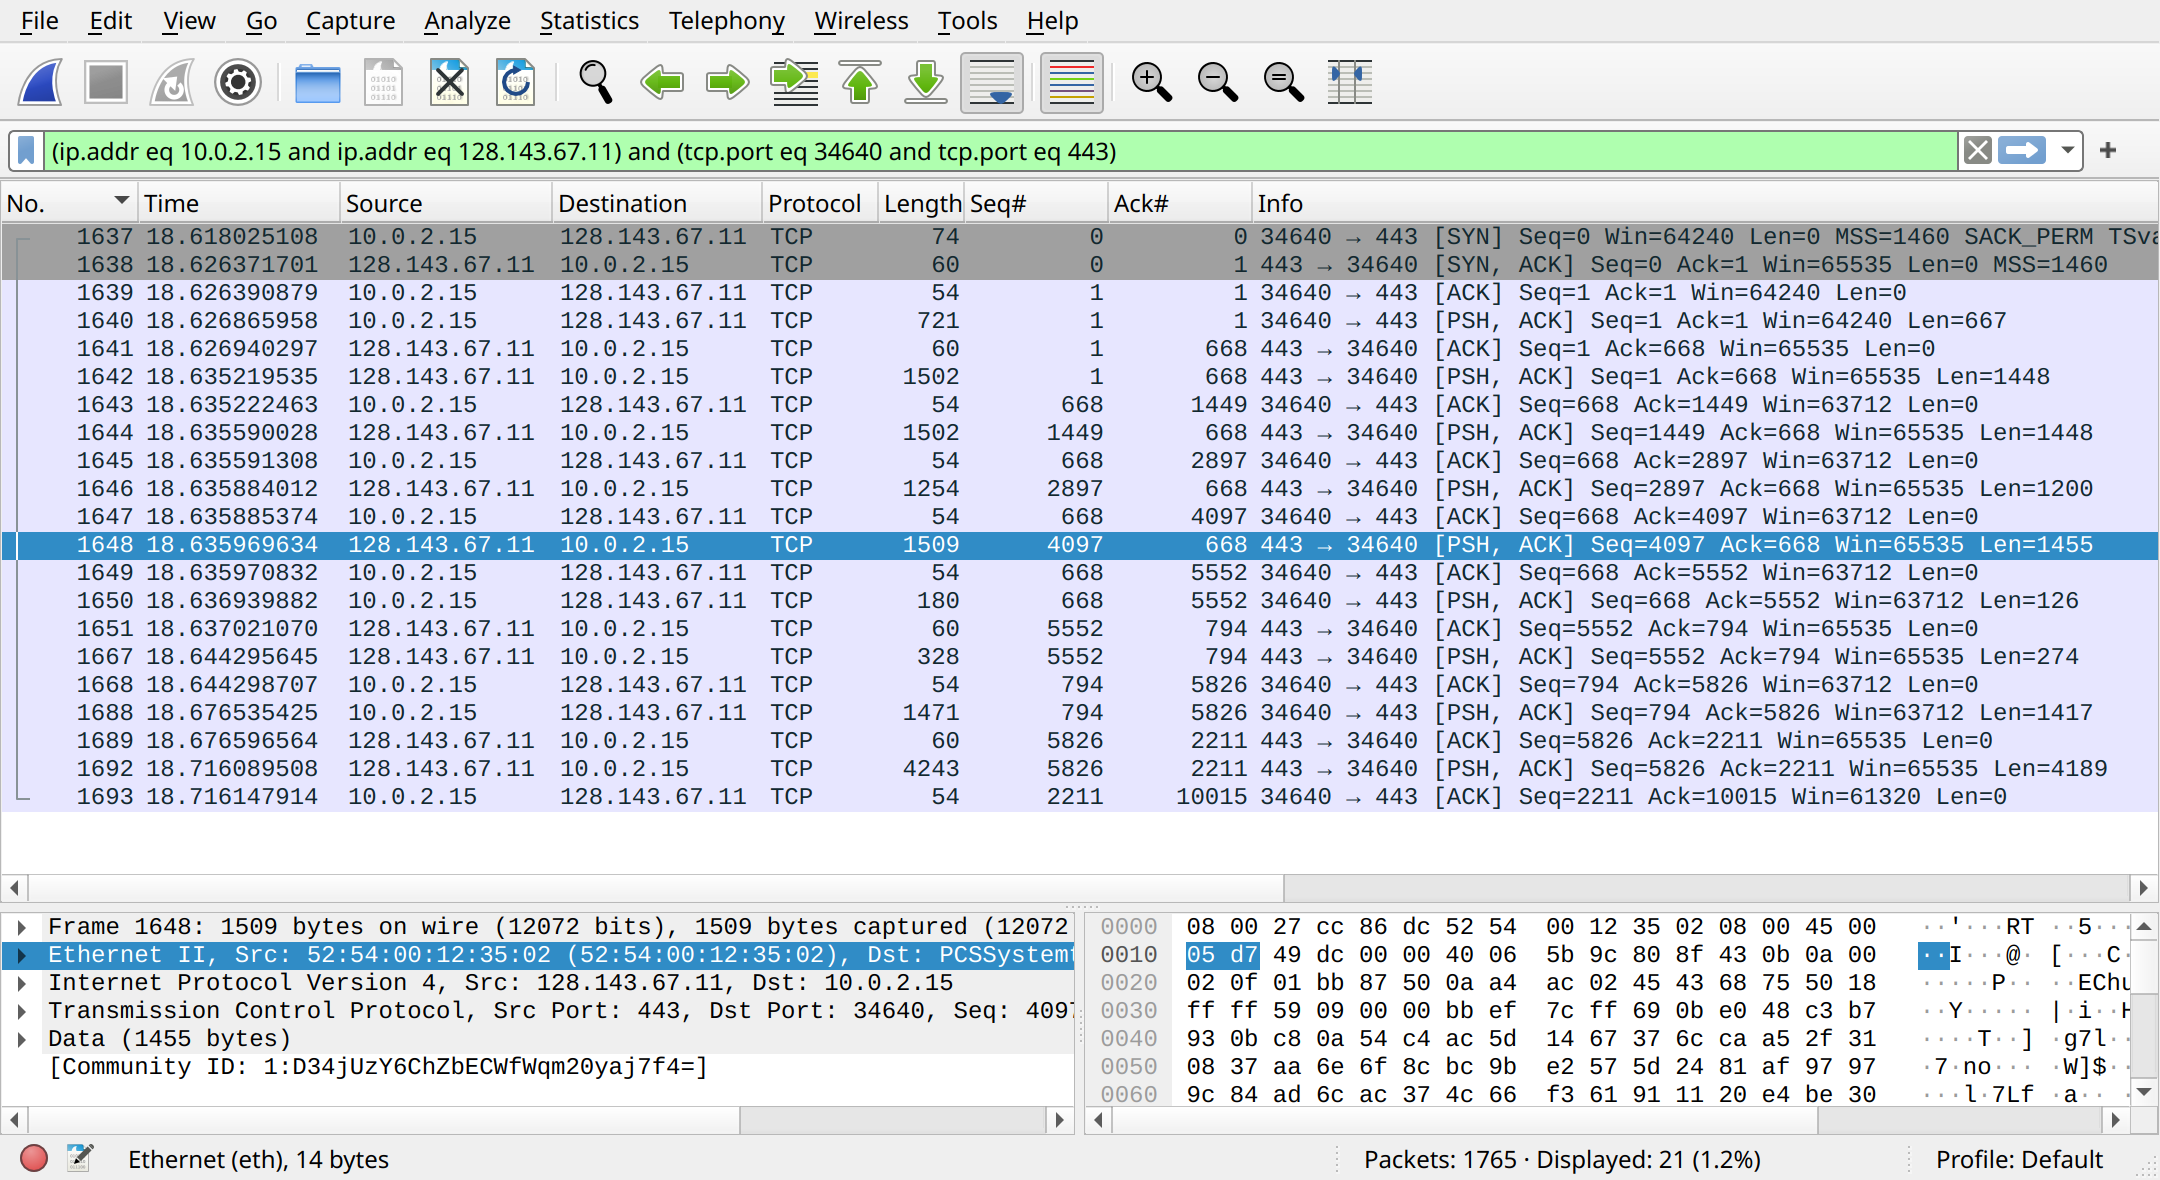
\includegraphics[width=\textwidth]{../reliable/wireshark-tcp-ex1-over}%
};
\path (0, 0) rectangle (14.5, -7); % for bounding box
\draw[overlay,help lines] (0, 0) grid (14, -8);
\begin{visibleenv}<2>

\end{visibleenv}
\end{tikzpicture}
\end{frame}


\subsection{TCP connection example}
\usetikzlibrary{shapes.geometric,spy}
\begin{frame}[fragile]{a TCP connection}
\tikzset{
    overlay box/.style={fill=white,fill opacity=0.95},
}
\begin{tikzpicture}[
    spy using outlines={%
        overlay,circle,magnification=2,size=2cm,connect spies,%
        every spy on node/.append style={very thick},%
        ultra thick,%
    }
]
\node[overlay,anchor=north west,inner sep=0mm] (base) at (0, 0) {%
\only<1-2>{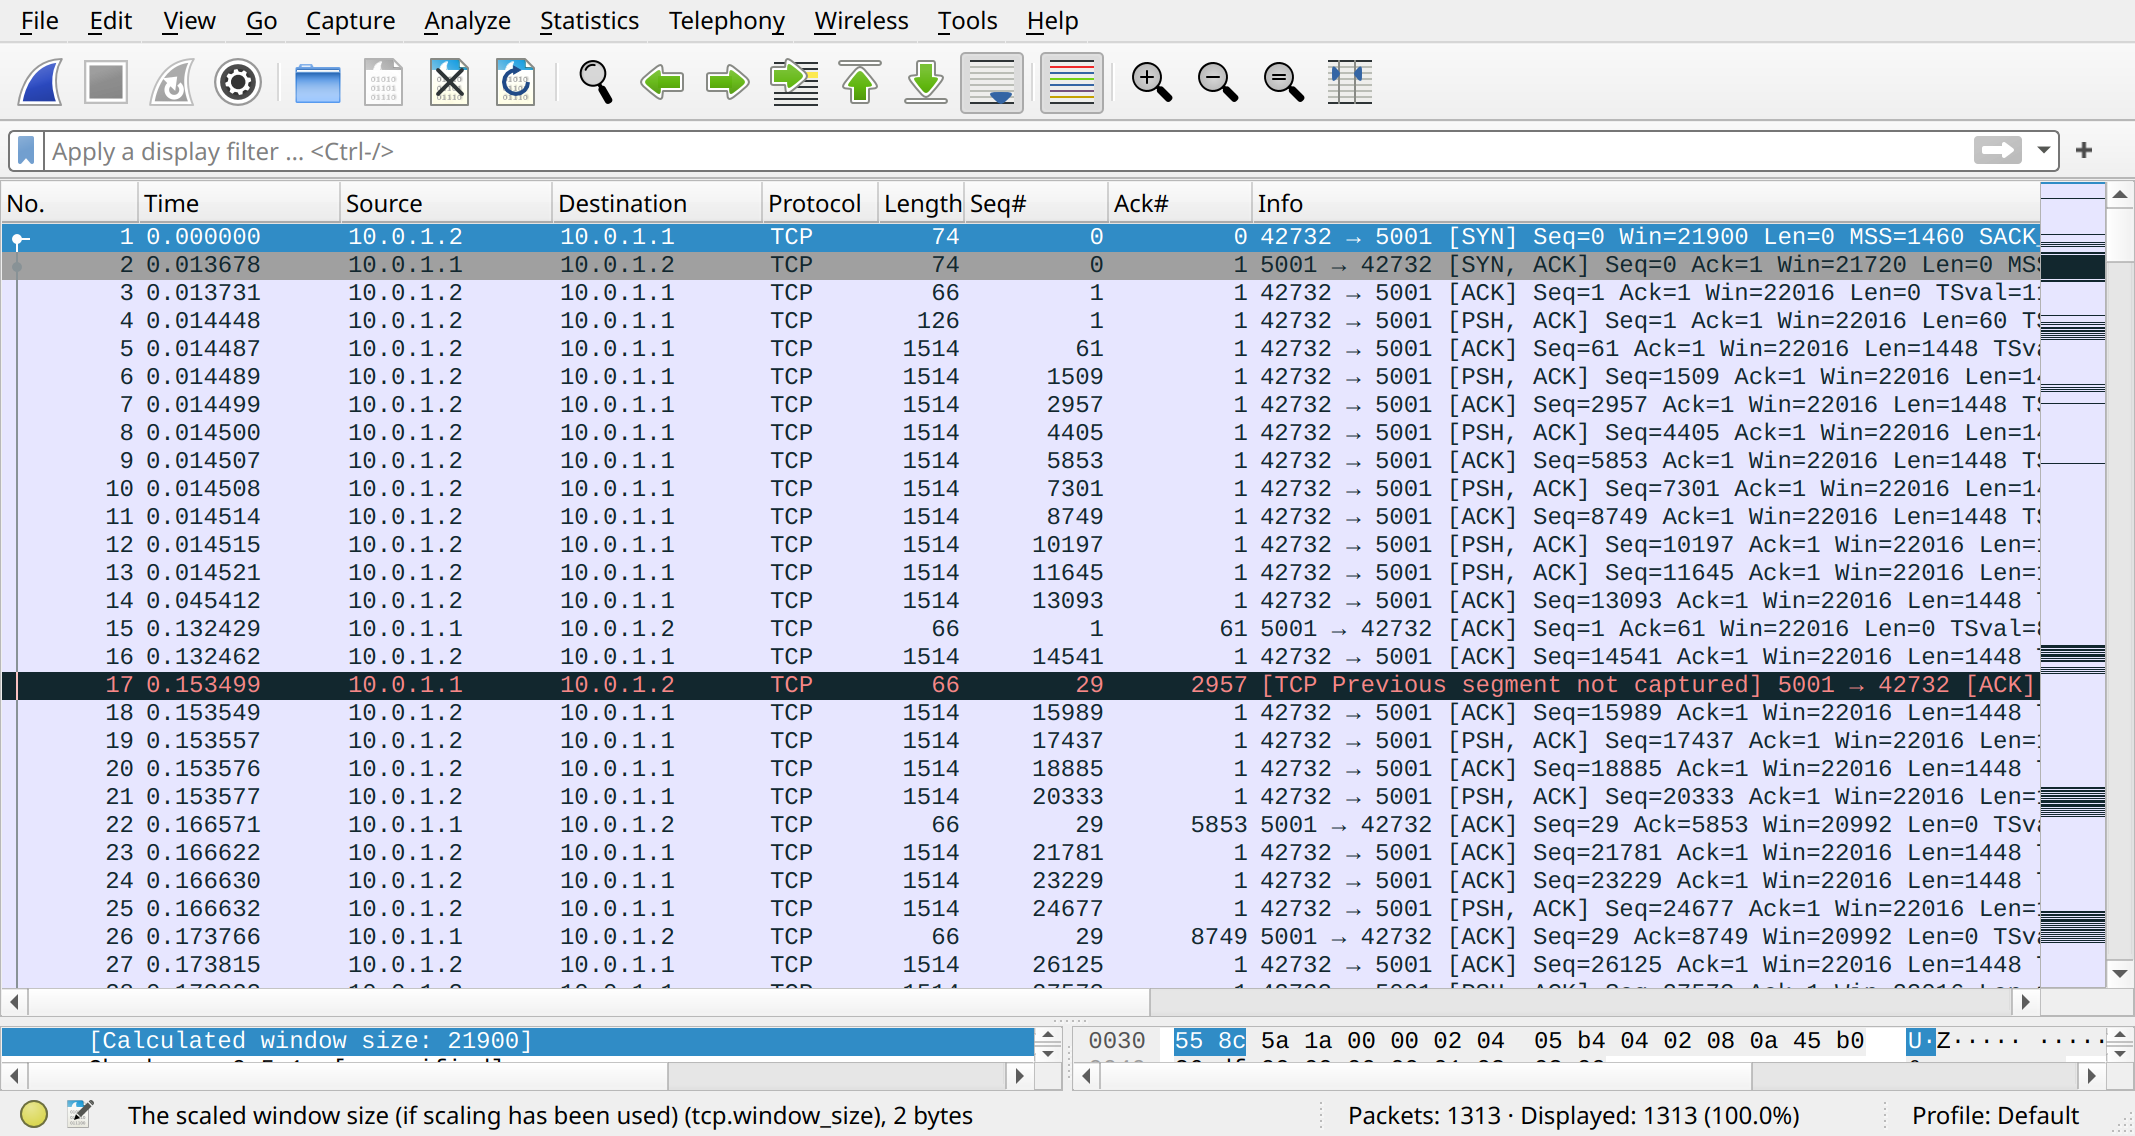
\includegraphics[width=\textwidth]{../reliable/wireshark-tcp-ex2-over}}%
\only<3->{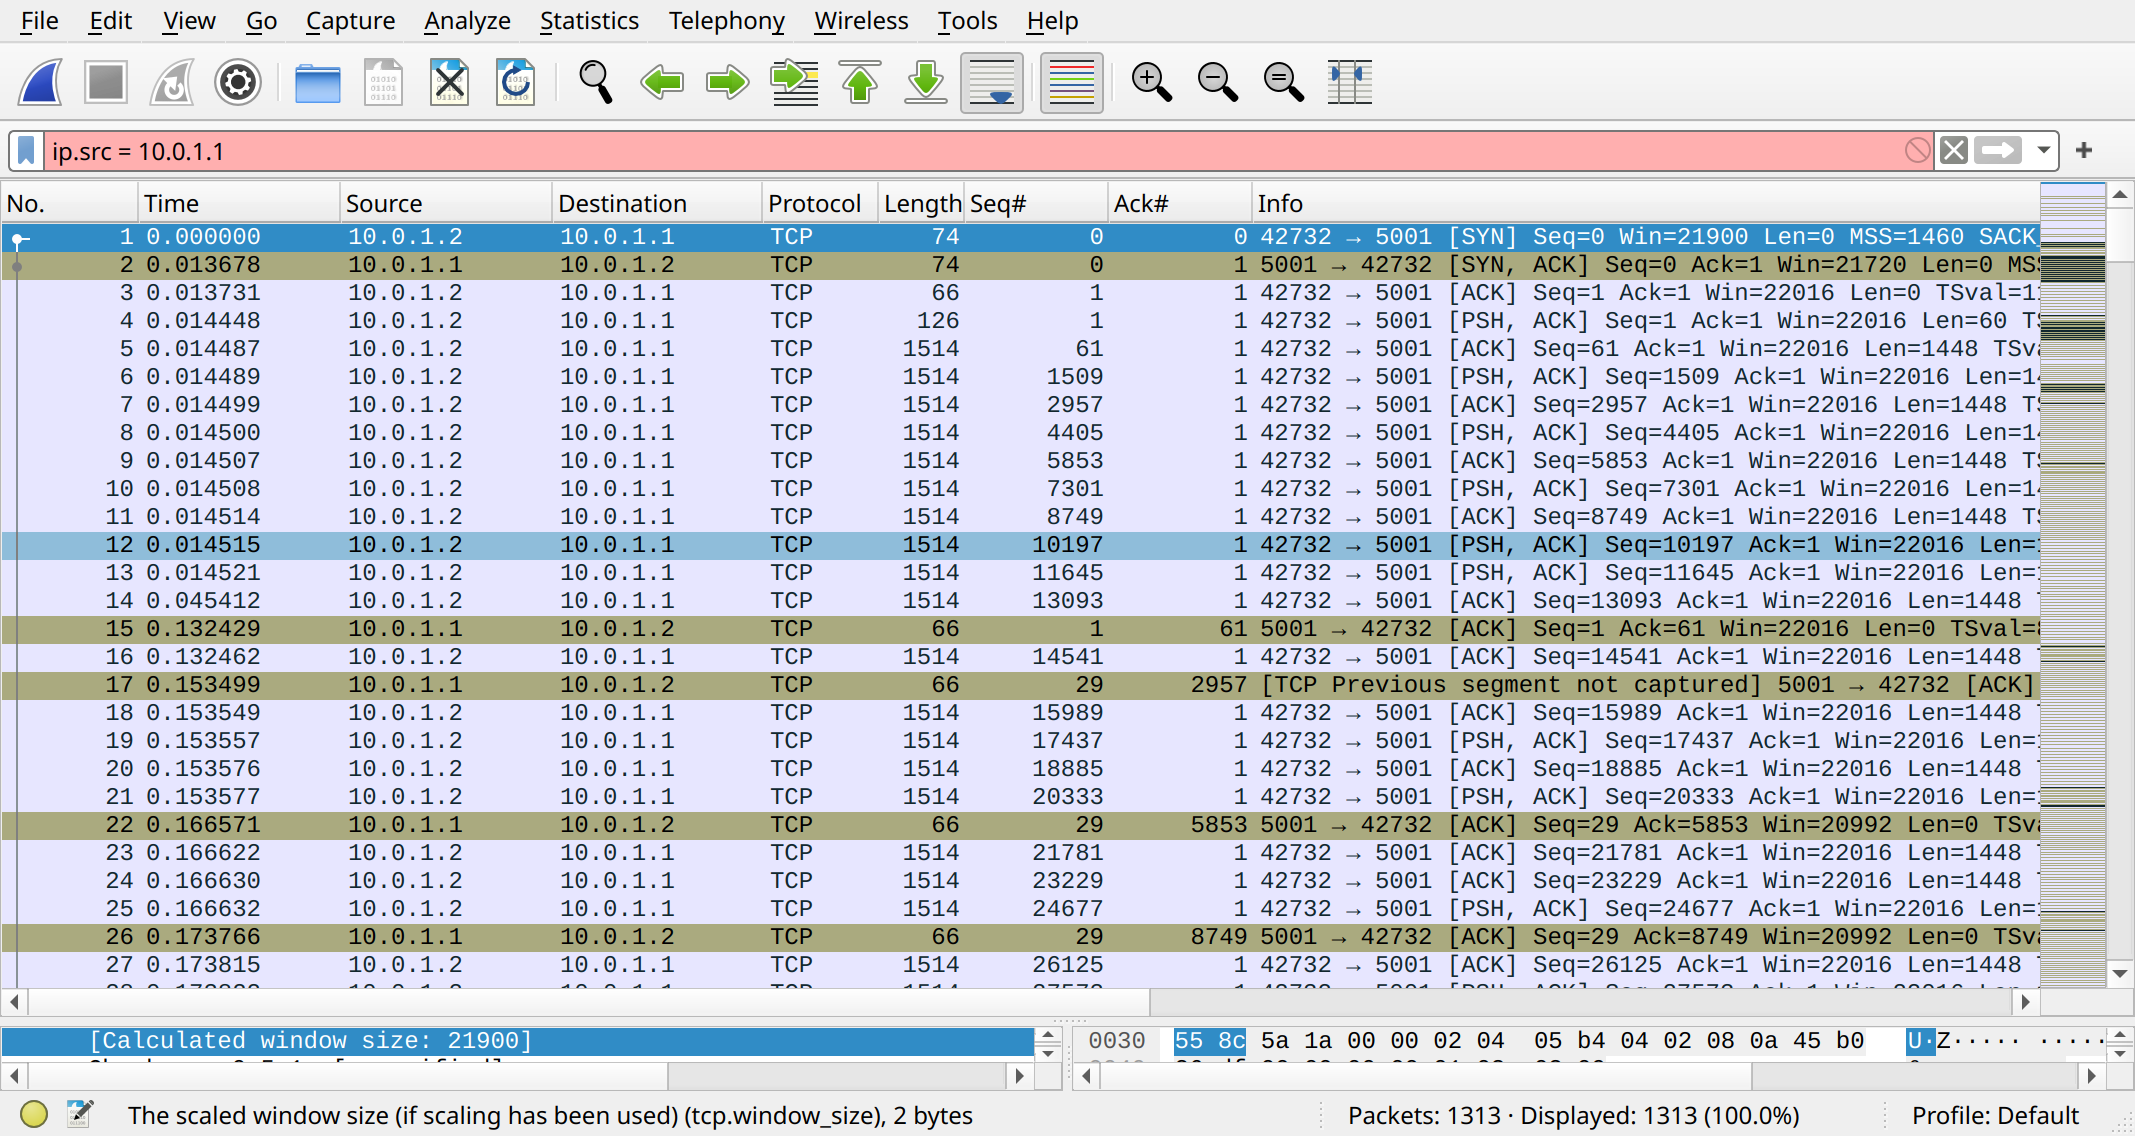
\includegraphics[width=\textwidth]{../reliable/wireshark-tcp-ex2-hi-dir}}%
};
\path (0, 0) rectangle (14.5, -7); % for bounding box
%\draw[overlay,help lines] (0, 0) grid (14, -8);
%\draw[overlay,help lines,dotted] (0, 0) grid[step=0.2] (14, -8);
\begin{visibleenv}<2-3>
\path[draw,red,very thick] (0, -1.5) rectangle (13.9, -2.125);
\node[red,overlay box,anchor=north,align=left] (c setup) at (6.95, -2.125) {
    connection setup, no data transferred 
};
\end{visibleenv}
\only<3>{\spy[rectangle,width=5cm,height=2.5cm,magnification=2] on (7.45, -1.7) in node at (12, 0);}
\begin{visibleenv}<3>
\node[overlay,overlay box,font=\small,anchor=east,align=left] at (9.5, -.5) {
    server+client sequence numbers \\
    advance by 1 to indicate where in setup
};
\end{visibleenv}
\begin{visibleenv}<4>
\path[draw,red,very thick] (0, -1.7) rectangle (13.9, -1.9);
\path[draw,red,very thick] (0, -4.2) rectangle (13.9, -4.39);
\path[draw,red,very thick] (0, -4.55) rectangle (13.9, -4.75);
\path[draw,red,very thick] (0, -5.5) rectangle (13.9, -5.75);
\path[draw,red,very thick] (0, -6.25) rectangle (13.9, -6.45);
\node[overlay box,align=left,anchor=north] at (6.95, -2.5) {
    connection is bidirectional \\
    from now, using olive color to show `backwards' packets
};
\end{visibleenv}
\only<5-6>{\spy on (7.25, -2.3) in node at (10, -1);}
\only<5-6>{\spy on (8, -4.3) in node at (12, -6);}
\begin{visibleenv}<5-6>
\path[draw,red,very thick] (6.55, -2.25 + .2) rectangle (7.5, -2.45 + .2);
    \node[overlay box,text=red,anchor=east,align=left] at (6.55, -2.35) {
        data packet with \\
        client bytes 1--60
    };
\path[draw,red,very thick] (7.55, -4.2) rectangle (8.5, -4.4);
    \node[overlay box,text=red,anchor=east,align=left] at (6.55, -4.3) {
        acknowledgement of \\
        client bytes up to 60
    };
\end{visibleenv}
\begin{visibleenv}<6>
\path[draw,red,very thick] (0, -2.25) rectangle (1.9, -2.45);
\path[draw,red,very thick] (0, -4.2) rectangle (1.9, -4.4);
\path[draw,red,dotted,double,ultra thick] (1, -2.45) -- (1, -4.2) node[midway,font=\small,fill=white,fill opacity=0.957,text=red,text opacity=1.0] {118 ms};
\end{visibleenv}
\begin{visibleenv}<7>
\path[draw,red,very thick] (12.6, -4.15) rectangle (13.3, -4.4);
\path[draw,red,very thick] (6.55, -4.2) rectangle (7.55, -4.4);
\path[draw,red,very thick] (6.55, -4.55) rectangle (7.55, -4.75);
\path[draw,red,very thick] (8.5, -4.55) rectangle (12, -4.75);
\only<7>{\spy[rectangle,width=10cm,magnification=1.5,height=1cm] on (10, -4.5) in node};
    \node[overlay box,text=red,anchor=south,align=left] at (6.55, -3.7) {
        jumps from server byte 0 to server byte 28 \\
        with no data sent \\
        wireshark IDs as missing packet
    };
% FIXME:  hilite len =0 and seq # 29
% FIXME: note missing data packet with bytes 1--28
% FIXME: screenshot scrolled down showing that
\end{visibleenv}
\end{tikzpicture}
\end{frame}

\begin{frame}[fragile]{a TCP connection}
\tikzset{
    overlay box/.style={fill=white,fill opacity=0.95},
}
\begin{tikzpicture}[
    spy using outlines={%
        rectangle,magnification=1.5,height=1cm,width=10cm,connect spies,%
        every spy on node/.append style={very thick},%
        ultra thick,%
    }
]
\node[overlay,anchor=north west,inner sep=0mm] (base) at (0, 0) {%
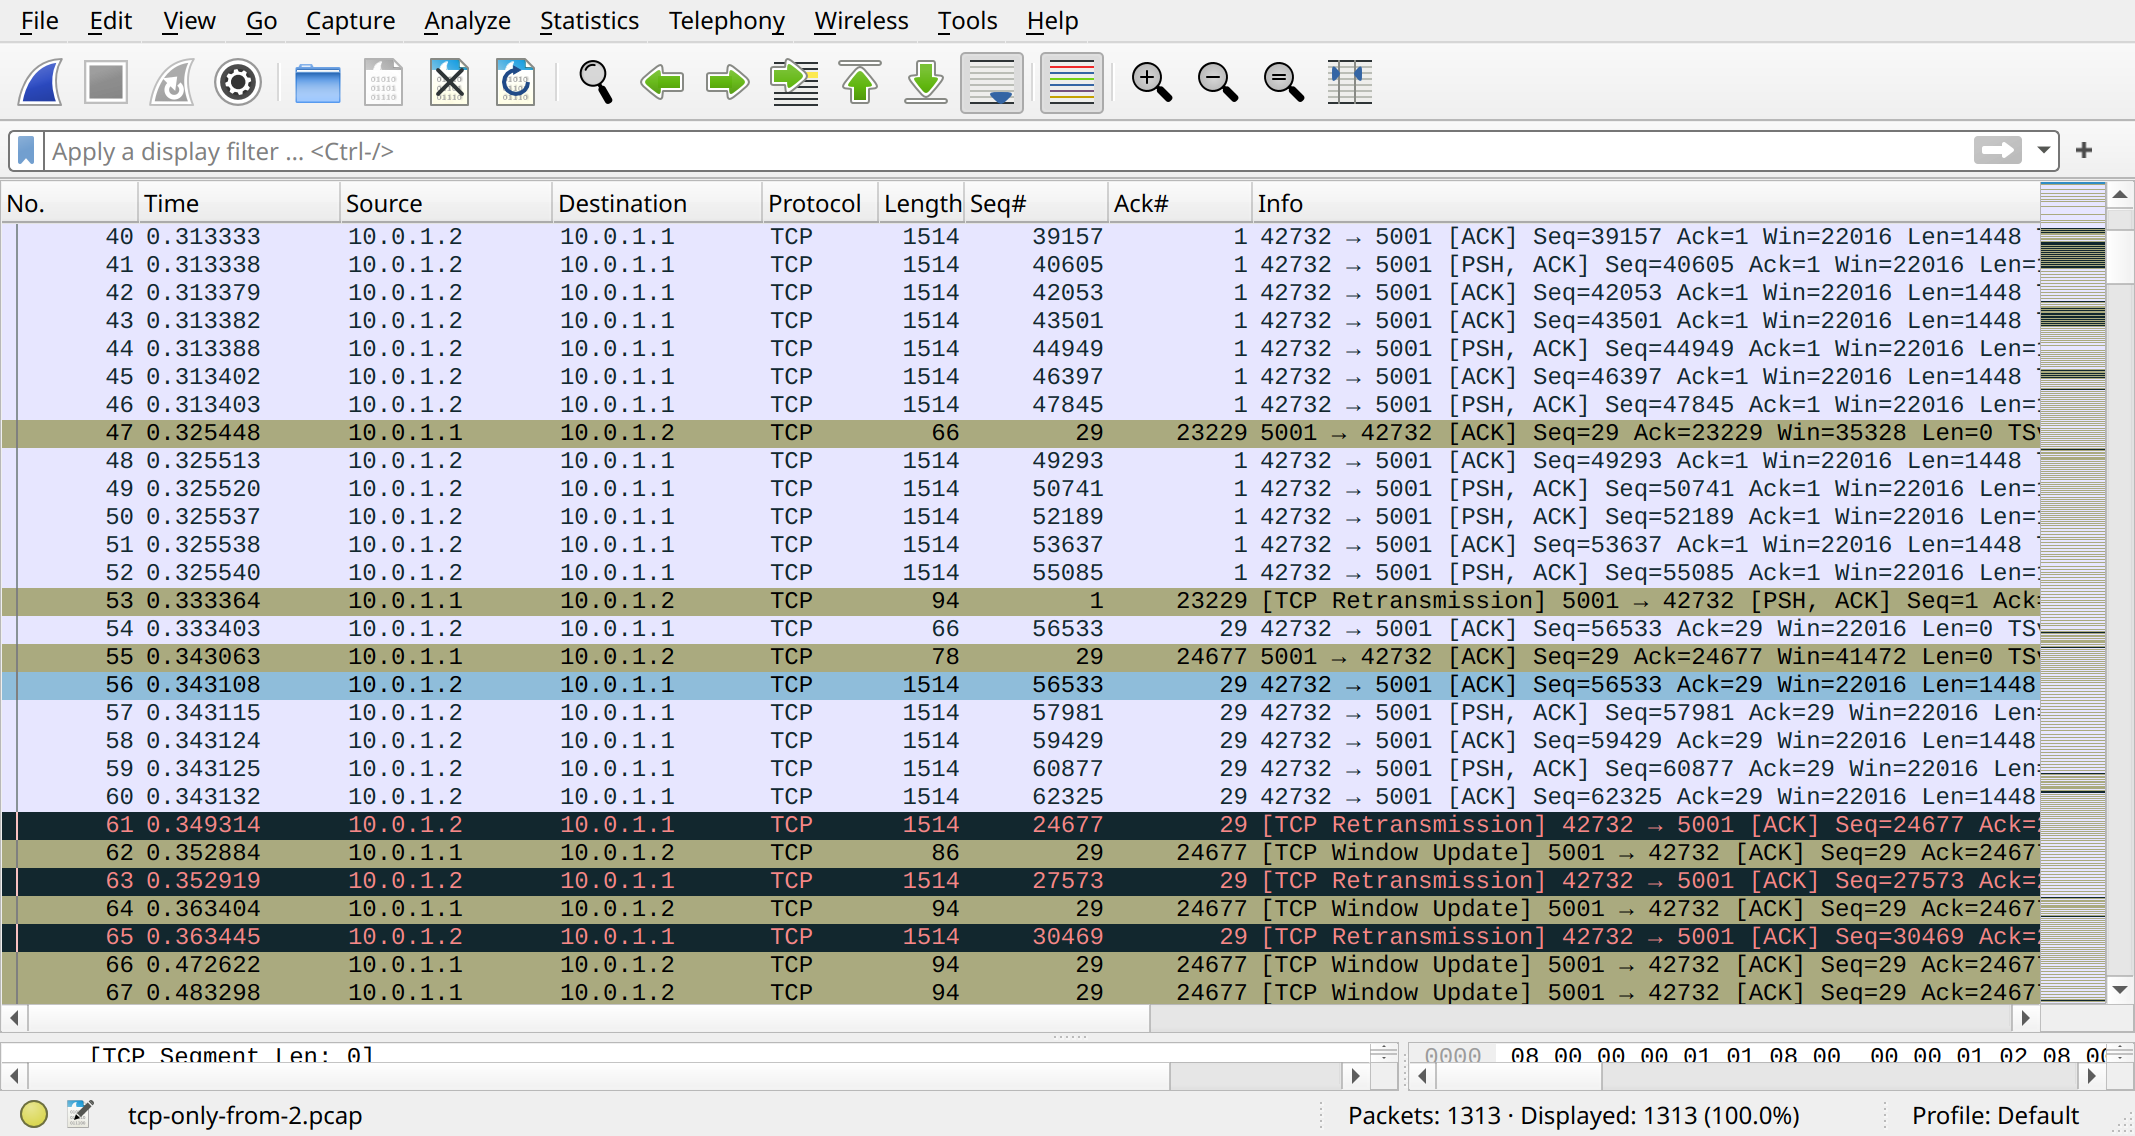
\includegraphics[width=\textwidth]{../reliable/wireshark-tcp-ex2-scrolled-server-retrans}%
};
\path (0, 0) rectangle (14.5, -7); % for bounding box
\spy on (10, -4.0) in node;
    \node[overlay box,text=red,anchor=south,align=left] at (6.55, -3.5) {
        scrolling down reveals retransmission later
    };
    \node[overlay box,text=black,font=\small,anchor=north,align=left] at (6.55, -4.5) {
        wireshark knows it's retransmission because \\
        sequence number sent by server went backwards
    };
\end{tikzpicture}
\end{frame}

\begin{frame}{first data packet}
\begin{tikzpicture}
\tikzset{
    overlay box/.style={fill=white,fill opacity=0.95},
}
\node[overlay,anchor=north west,inner sep=0mm] (base) at (0, 0) {%
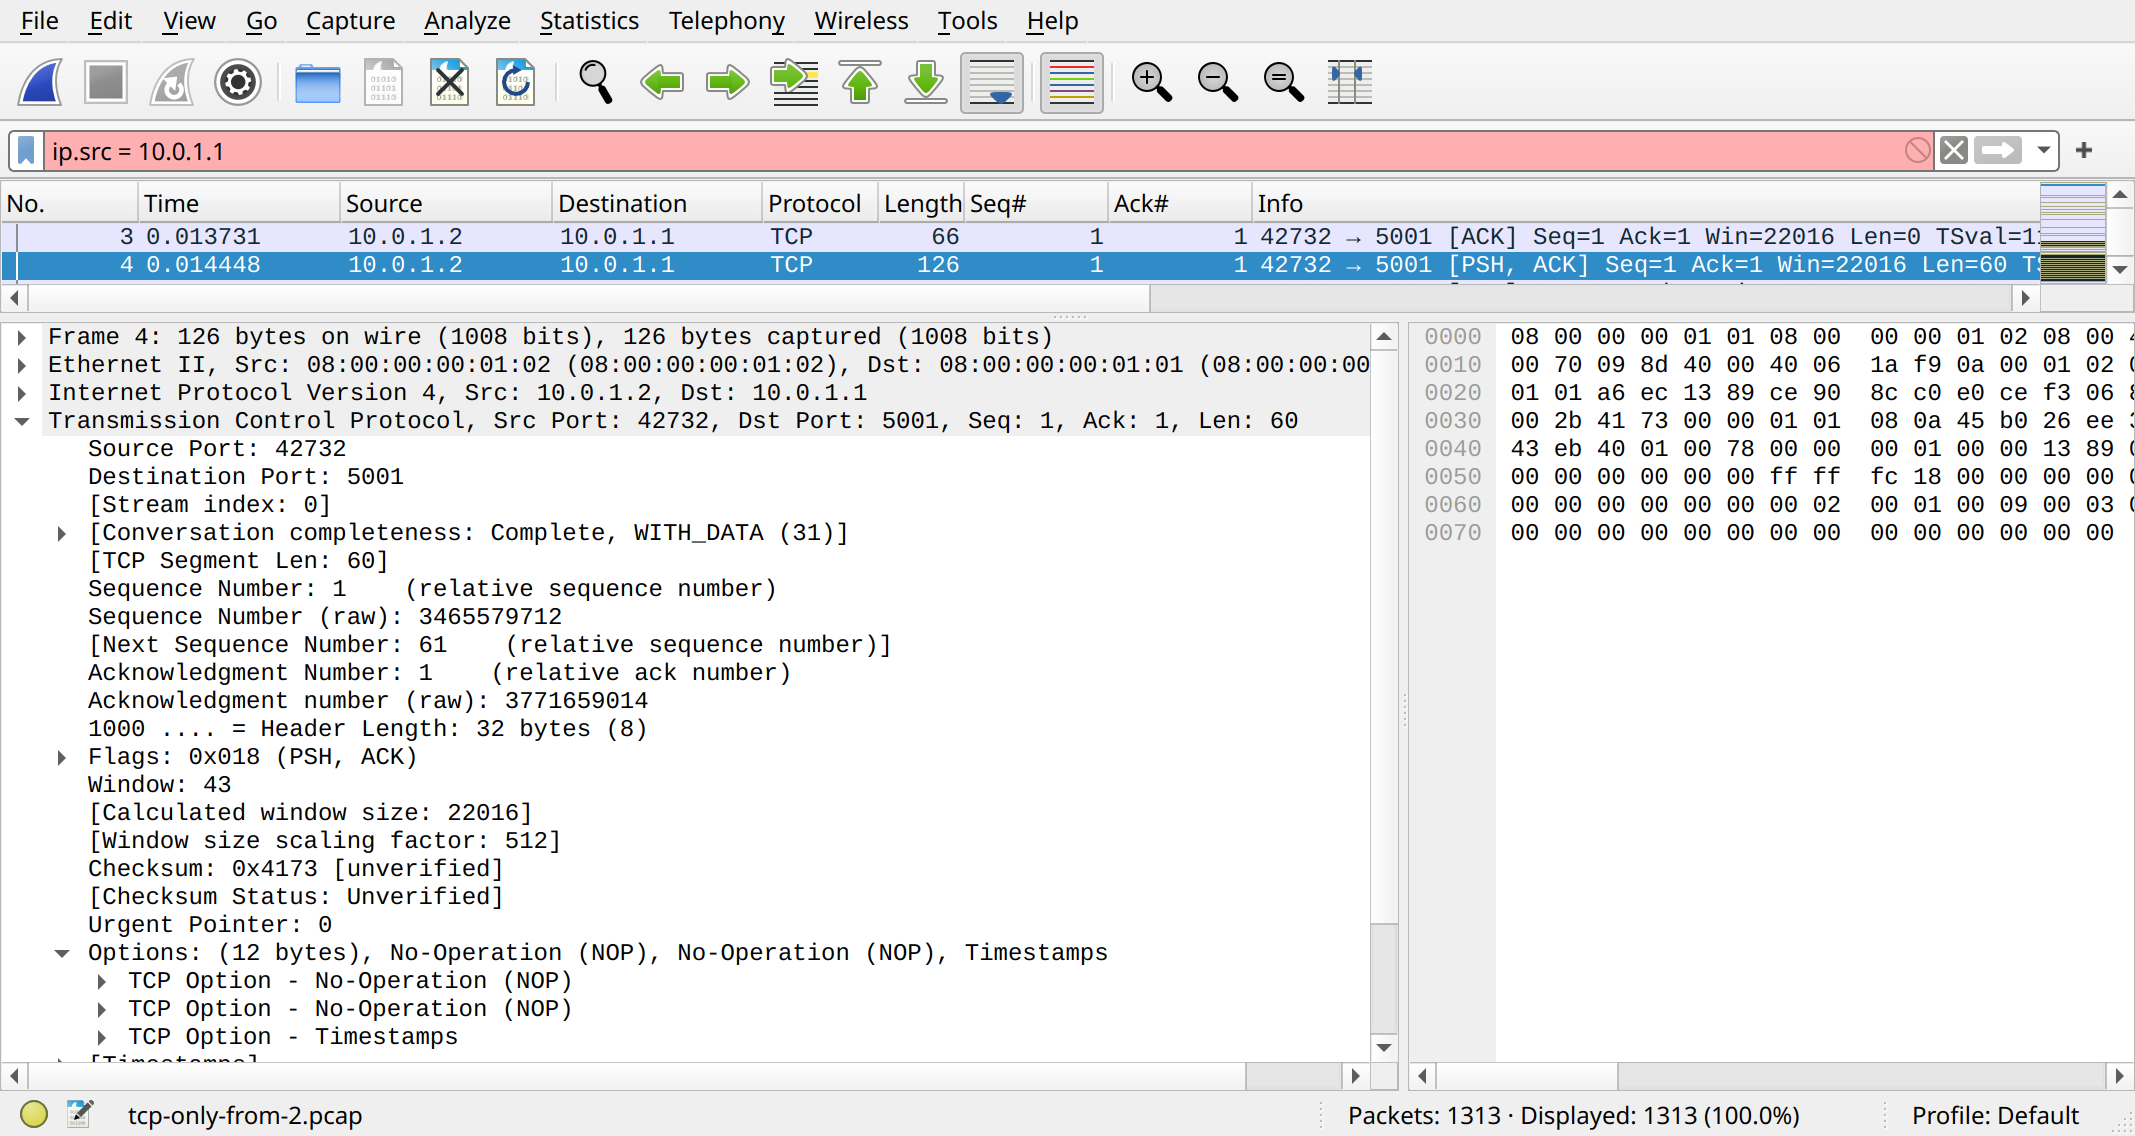
\includegraphics[%
    width=\textwidth,%
    % left bottom right top
    trim={0.5cm 2cm 20cm 10cm},clip,%
]{../reliable/wireshark-tcp-ex2-firstdata}%
};
\path (0, 0) rectangle (14.5, -7); % for bounding box
\draw[violet,overlay,help lines] (0, 0) grid (14, -8);
\draw[violet,overlay,help lines,dotted] (0, 0) grid[step=0.2] (14, -8);
%\spy[overlay,rectangle,magnification=1.7,height=7.5cm,width=10cm] on (3, -5) in node at (9, -3.5);
\begin{visibleenv}<2>
    \draw[red,very thick] (0.65, -2.45) rectangle (3.5, -2.75);
    \node[overlay box,text=red,anchor=west,align=left] at (3.5, -2.6) {
        not actually part of header \\
        computed using length from lower layer
    };
\end{visibleenv}
\begin{visibleenv}<3>
    \draw[red,very thick] (0.65, -2.75) rectangle (8.2, -3.25);
    \node[overlay box,text=red,anchor=north west,align=left] at (0.65, -3.25) {
        sequence numbers in header don't start at 0 \\
        wireshark converts to 0-based indices
    };
\end{visibleenv}
\begin{visibleenv}<4>
    \draw[red,very thick] (0.65, -2.75) rectangle (8.2, -3.55);
    \node[overlay box,text=red,anchor=north west,align=left] at (0.65, -3.55) {
        sequence number is \textit{first} byte being sent \\
        need to use segment length to know last byte's number \\
        (= what to ACK if receiving this)
    };
\end{visibleenv}
\begin{visibleenv}<5>
    \draw[red,very thick] (0.65, -3.55) rectangle (7.3, -4);
    \node[overlay box,text=red,anchor=north west,align=left] at (0.65, -4) {
        ack number indicates received start-of-connection stuff \\
        and nothing else (in case server sent something)
    };
\end{visibleenv}
\begin{visibleenv}<6>
    \draw[red,very thick] (0.65, -4.3) rectangle (3.85, -4.6);
    \node[overlay box,text=red,anchor=north west,align=left] at (0.65, -4.6) {
        PSH = no more data right now \\
        ACK = acknowledgment number is valid 
    };
\end{visibleenv}
\begin{visibleenv}<7>
    \draw[red,very thick] (0.65, -4.55) rectangle (5.15, -5.35);
    \node[overlay box,text=red,anchor=south west,align=left] at (0.7, -4.5) {
        window scaling option in use \\
        (scaling factor only sent in connection setup)
    };
\end{visibleenv}
\begin{visibleenv}<8>
    \draw[red,very thick] (0.65, -6.1) rectangle (10.3, -7.2);
    \node[overlay box,text=red,anchor=south west,align=left] at (0.7, -6.0) {
        no-operation options used to make TCP header size multiple of 4
    };
\end{visibleenv}
\end{tikzpicture}
\end{frame}

\begin{frame}{sequence numbers graph}
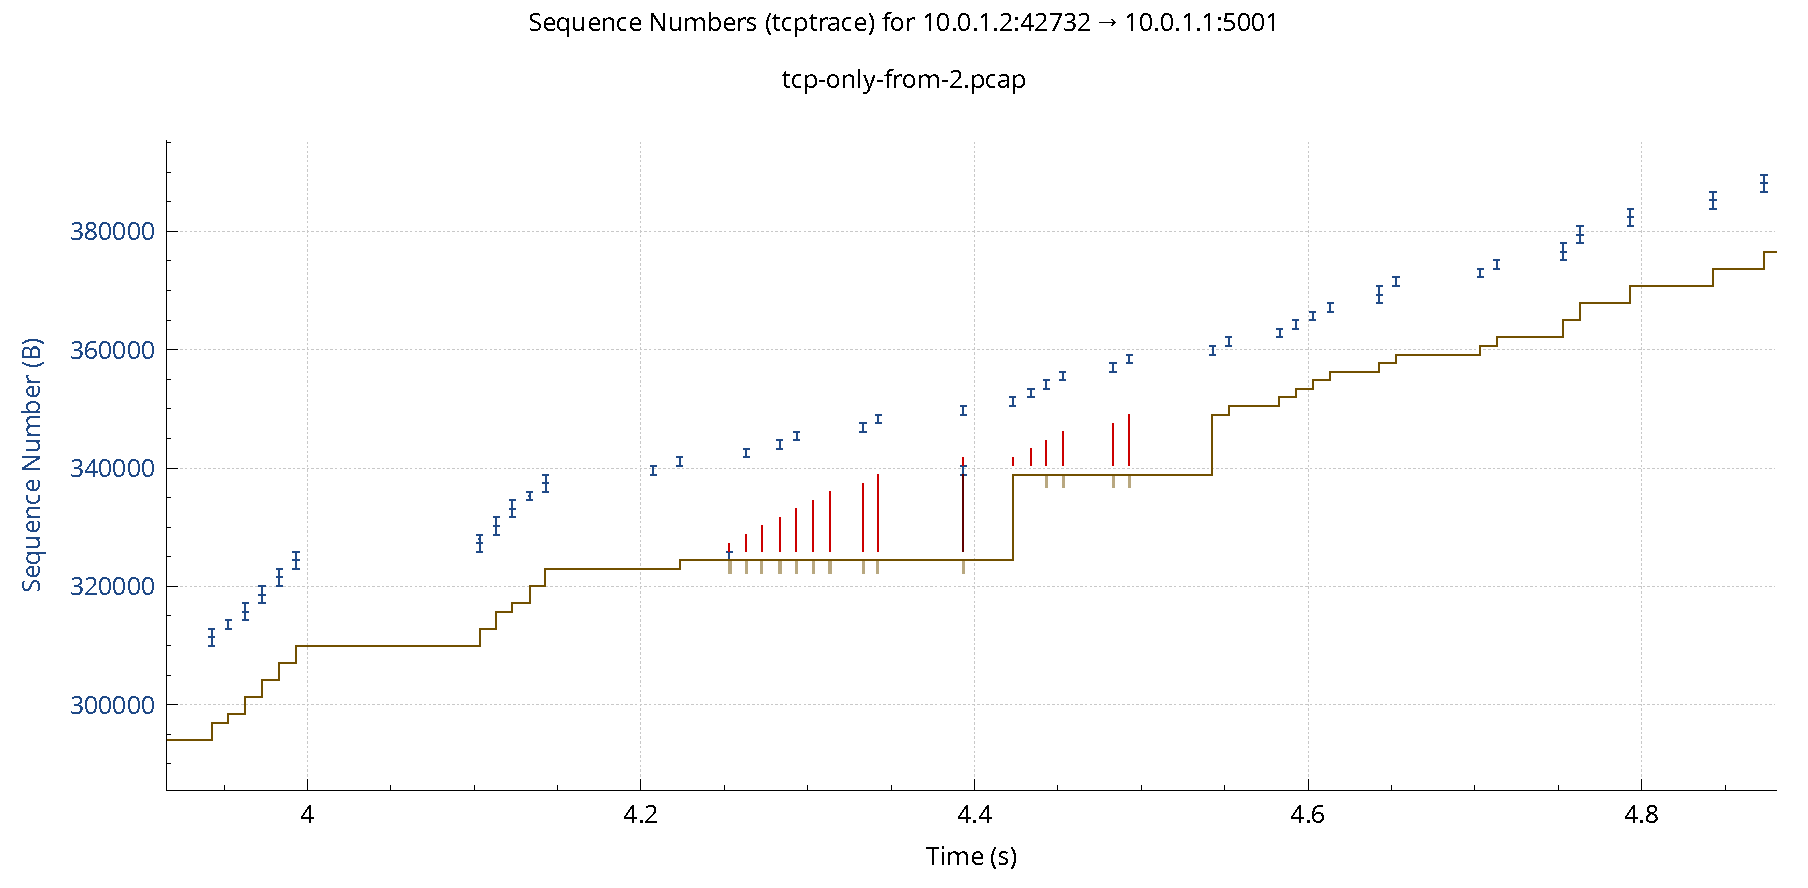
\includegraphics[width=\textwidth]{../reliable/tcptrace-example2}
% FIXME: line at bottom = acknowledgment number from server
% FIXME: blue "I"s = data packets sent
% FIXME: notches on acknowledgment line = duplicate acknowledgments
% FIXME: red lines = selective acknowledgment info
% FIXME: note --- sending new packets triggered by ACK
    % and this is observed from the client
    % so each blue line matches a red line
% FIXME: note slowdown due to congestion
\end{frame}

\begin{frame}{reading thigs graph}
    \begin{itemize}
    \item bottom line = last ack number
    \item notches on bottom line = duplicate acks
    \item red lines = selective ACK info
    \end{itemize}
\end{frame}

\begin{frame}{diff. timing in opposite direction}
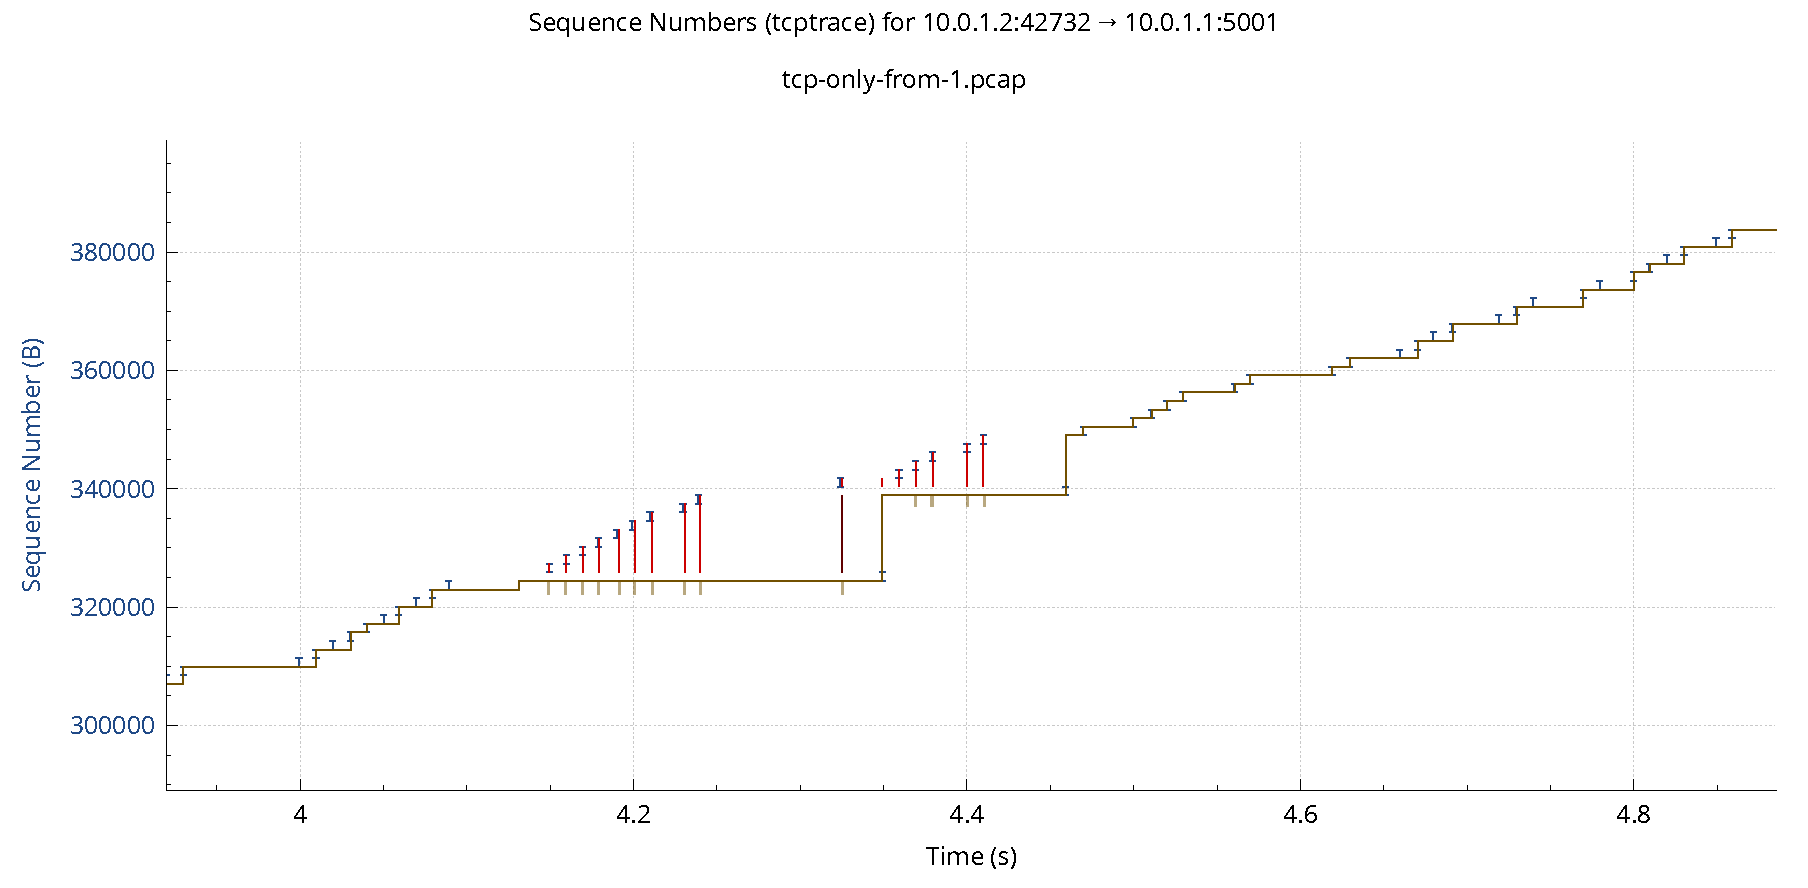
\includegraphics[width=\textwidth]{../reliable/tcptrace-example2-oppdir}
% FIXME: note different timing
\end{frame}



